\documentclass[12pt, a4paper, oneside]{book}   	% document style definition


\usepackage{hslu}                               % apply HSLU style
\usepackage{comment}                            % having comment sections \begin{comment} \end{comment}
\usepackage[utf8]{inputenc}						% charactere interpretation
\usepackage{amsmath}							% math package
\usepackage{amsfonts}							% font package for math symbols
\usepackage{amssymb}							% symbols package - definition of math symbols
\usepackage{listings}							% package for code representation

\usepackage{csquotes}       % Quotation support
\usepackage[style=apa,backend=biber]{biblatex}       % Bibliography, 
\DeclareLanguageMapping{american}{american-apa}
\addbibresource{references.bib} % Bibliography file

\usepackage{graphicx}							% for inclusion of image
\setlength {\marginparwidth }{2cm}
\usepackage{todonotes}
\renewcommand{\todo}[1]{\textcolor{red}{TODO: #1}}
%\presetkeys{todonotes}{inline, textcolor=red, color=none, noinlinepar}{}

%\let\todoold\todo
%\newcommand{\todo}[1]{\textcolor{red}{TODO: #1}\todo[prepend, caption={TODO: #1}]{}}

%\renewcommand{\todo}[1]{\todo[inline]{\textcolor{red}{TODO: #1}}}
%\renewcommand{\todo}[1]{\todo{\textcolor{red}{TODO: #1}}}




\usepackage{booktabs}       % Better tables
\usepackage{caption}        % Better captions
\usepackage{subfig}								% to arrange figures next to each other
\usepackage{float}								% text style surrounding images
\usepackage{threeparttable}
\usepackage{tikz}								% used to place logos on title page
% \usepackage{gensymb}							% for special characters such as °
\usepackage{titlesec}
\usepackage{multirow}
\usepackage{siunitx}
\usepackage{tabularx}
\usepackage{tikzscale}
\usepackage{csvsimple}

\usepackage{enumitem}

\setlist[itemize]{itemsep=3pt, parsep=0pt}
\setlist[enumerate]{itemsep=3pt, parsep=0pt}


\usepackage{appendix}

% PDF/A Compliance, todo: enable and remove hyperref usepackage afterwards
% \usepackage[a-1b]{pdfx}
% \catcode30=12

\usepackage{hyperref}
\hypersetup{hidelinks}

\newcommand{\linkchap}[1]{\hyperref[#1]{chapter~\ref{#1}~\nameref{#1}}}
\newcommand{\linkapp}[1]{\hyperref[#1]{appendix~\ref{#1}~\nameref{#1}}}

\usepackage[acronym]{glossaries}         				% package for glossary

\setcounter{tocdepth}{1}                        % hide subsections from TOC
\makenoidxglossaries
\newacronym{HSLU}{HSLU}{Lucerne University of Applied Sciences and Arts}
\newacronym[see={[Glossary:]{fitzpatrick-skin-type}}]{FST}{FST}{Fitzpatrick skin type\glsadd{fitzpatrick-skin-type}}
\newacronym{ML}{ML}{Machine Learning}
\newacronym{AI}{AI}{Artificial Intelligence}
\newacronym{FPR}{FPR}{false positive rate}
\newacronym{TPR}{TPR}{true positive rate}
                                % include acronyms.txt file
\newglossaryentry{fitzpatrick-skin-type}{
	name={Fitzpatrick skin type},
	plural={Fitzpatrick skin types},
	description={A skin classifier based on the skins' reaction to ultraviolet light, developed by dermatologist Dr. Thomas Fitzpatrick \autocite{Gottfrois2024}}
}
\newglossaryentry{JupyterNotebook}{
	name={Jupyter Notebook},
	description={Executable files, often used in ML to write Python code and add explanations in text form}
}
\newglossaryentry{gpuhub}{
	name={GPUhub},
	description={\gls{HSLU}’s server infrastructure for GPU-related computing. It provides isolated environments with JupyterLab access for developing and running \gls{ML} workflows}
}
\newglossaryentry{pediatric}{
	name={pediatric},
	description={A medical term for infants, children and adolescents \autocite{Farlex_nodate}}
}
\newglossaryentry{proxyVar}{
	name={proxy variable},
	plural={proxy variables},
	description={"one or more variables that encode the protected attribute with a substantial degree of accuracy" \autocite{Wang_2021}}
}
\newglossaryentry{teledermatology}{
	name={teledermatology},
	description={dermatological care from a distance, supported by modern technology \autocite{Pala_2020}}
}
\newglossaryentry{Fairlearn}{
	name=Fairlearn,
	description={A Python library for assessing and improving fairness in machine learning models. It supports various fairness metrics and mitigation techniques, especially for binary classification tasks \autocite{Fairlearn_nodate}}
}
\newglossaryentry{Equalized-Odds-Difference}{
	name={equalized odds difference},
	description={The absolute difference in true positive and false positive rates between subgroups, used as a group fairness metric \autocite{Fairlearn_nodate}}
}
\newglossaryentry{Equalized-Odds-Ratio}{
	name={equalized odds ratio},
	description={The ratio of true positive and false positive rates between subgroups, used as a group fairness metric \autocite{Fairlearn_nodate}}
}                                % include glossary.txt file
\graphicspath{{figures/}}						    % set path of graphics folder



% Format chapter titles without "Chapter X" prefix
\titleformat{\chapter}[hang]
{\normalfont\LARGE\bfseries}  % Style: Large bold text
{\thechapter}                 % Number format: Just the number
{1em}                         % Space between number and title
{}                            % Code before the title (empty)

\titlespacing*{\chapter}
{0pt}
{-20pt}
{30pt}

% changed paragraph and subsection appearance
\setcounter{secnumdepth}{3}
\renewcommand{\paragraph}[1]{%
	\subsubsection*{#1}%
%	\addcontentsline{toc}{subsection}{#1}%
}


% mentioned in header
\newcommand{\tblWidthDescription}{\hsize=0.6\hsize\raggedright}
\newcommand{\tblWidthContext}{\hsize=0.18\hsize}
\newcommand{\tblWidthDescriptionLong}{\hsize=0.73\hsize\raggedright}
\newcommand{\tblWidthContextShort}{\hsize=0.09\hsize}

%improved basic functionality
\newcommand{\bolditalic}[1]{\textbf{\textit{{#1}}}}

%indicate citations
% Define a flag to track whether we're inside a raw citation block
\newif\ifrawcitationactive
\rawcitationactivefalse % Default: Not inside a raw citation block

% Define color commands with conditional checking
\newcommand{\rawcitationstart}{
	\color{purple}\rawcitationactivetrue
}
\newcommand{\rawcitationend}{
	\color{black}\rawcitationactivefalse
}

\newcommand{\rawcitationusedstart}{\color{violet}}
\newcommand{\rawcitationusedend}{%
	\ifrawcitationactive
	\color{purple}  % If inside rawcitation, reset to purple
	\else
	\color{black}  % Otherwise, reset to black
	\fi
}


% indicate info about criteria
\newcommand{\baaCriteria}[1]{\textcolor{blue}{#1}}


%----------------------------------------------------------------------------------------
%	DOCUMENT INFORMATION
%----------------------------------------------------------------------------------------
\author{Nadja Stadelmann}                       % author name
\city{Lucerne (Switzerland)}                    % author's place of origin
\title{Demographic Biases in Dermatology~Models}   % thesis title
\subtitle{\large}               % thesis subtitle

\date{2025}                                     % the year when the thesis was written (for the titlepage)
\defensedate{June 23th, 2025}                % the date of the private defense
\defencelocation{Lucerne}                       % location of defence
\extexpert{Dr. Jürg Schelldorfer}                         % name of external expert
\indpartner{Applied AI Research Lab}                       % name of industry partner

% jury, supervisor and dean are only relevant if acceptance sheet is enabled with the next line
% \acceptsheet
\jury{                                          % members of the jury
    \begin{itemize}
        \item Prof. Dr. Name Surname from Lucerne University of Applied Sciences and Arts, Switzerland (President of the Jury);
        \item Prof. Dr. Name Surname from Lucerne University of Applied Sciences and Arts, Switzerland (Thesis Supervisor);
        \item Prof. Dr. Name Surname from Lucerne University of Applied Sciences and Arts, Switzerland (External Expert).
    \end{itemize}
}

\supervisor{Dr. Ludovic Amruthalingam}             % name of supervisor
\dean{Prof. Dr. René Hüsler}                   % name of faculty dean

\acknowledgments{
	\noindent
	First and foremost, I would like to express my gratitude to Ludovic Amruthalingam for giving me the opportunity to work on this thesis and for his dedicated supervision throughout. His support, feedback, and guidance were invaluable to the successful completion of this work.\newline\hspace*{\parindent} 
	Many thanks go to Philippe Gottfrois, the main author of the PASSION project, for sharing valuable information and dermatology-specific insights, which was essential for my work.\newline\hspace*{\parindent} 
	I also thank Simone Lionetti for being ready to step in as deputy supervisor, helping with setting up the initial assignment and providing feedback.\newline\hspace*{\parindent} 
	As a LaTeX beginner, I am grateful to Pascal Baumann for his assistance, which made the learning process significantly smoother.\newline\hspace*{\parindent} 
	I would also like to acknowledge the broader research community working towards fairer and more accessible AI. Their efforts not only laid the groundwork for the concepts and metrics explored in this thesis, but contribute to address disparities in the current world. They inspire others for responsible innovation in machine learning.\newline\hspace*{\parindent} 
	Last but not least, I would like to thank my boyfriend, friends, family, and co-workers for their encouragement, patience, and emotional support. Special thanks to my mum and sister for their careful proofreading and helpful suggestions.\newline\hspace*{\parindent} 
	Your support made this thesis possible.
}

\sloppy
\begin{document}
	\english                                        % define thesis language: \german or \german
	\maketitle
	
	\todo{reenable in the end}
	%\tolerance=1
	%\emergencystretch=\maxdimen
	%\hyphenpenalty=10000
	%\hbadness=10000
	
	
	%----------------------------------------------------------------------------------------
	%	PREAMBLE
	%----------------------------------------------------------------------------------------
	
	\begin{abstractstyle}{AI Usage Declaration}
	\noindent
	To write this bachelor thesis, OpenAI’s language model ChatGPT (free version, GPT-3.5) to support specific tasks throughout the research and writing process. The assistance provided mainly included:
	
	\begin{itemize}
		\item Suggesting improvements for phrasing technical descriptions and argumentation clearly while preserving original content.
		\item Suggesting structures in the report.
		\item Summarizing text passages.
		\item Refining LaTeX formatting and ensuring structural 	consistency.
		\item Create initial code samples to remove boilerplate work during development.
	\end{itemize}
	\noindent
	The core research contributions and evaluations were carried out independently.
	\end{abstractstyle}
	
	
	\begin{abstractstyle}{Abstract}
	   \noindent
	   Skin diseases affect up to 80\% of children and adolescents in Sub-Saharan Africa, yet dermatology treatment remains often inaccessible, with fewer than one dermatologist per million inhabitants. AI-supported teledermatology can offer a potential solution, for example by enabling early triage of skin conditions. However, current AI models often perform poorly on highly pigmented skin due to demographic biases in current dermatology datasets, which predominantly contain images of low pigmented skin. The PASSION project addresses this gap by building a dataset focused on patients with highly pigmented skin in Sub-Saharan Africa to reduce demographic bias in dermatology AI models.
	   
	   This thesis evaluates the effectiveness of bias mitigation strategies in the PASSION context. A structured methodology was followed, including a contextualized literature review on biases, fairness and mitigation methods in medical AI, analysis of metadata completeness and representation of demographic groups in the PASSION dataset, and development of a reproducible fairness assessment pipeline. Subgroup fairness was analyzed using equalized odds, a metric that accounts for both true and false positives, which is crucial to detect systematic diagnosis errors. Stratified splitting was applied as a mitigation method to validate the newly established fairness assessment pipeline.
	   
	   Reproducing PASSION's results involved resolving metadata linkage issues, including outdated file references that required manual correction. Due to time and resource constraints, the focus shifted from testing multiple mitigation methods to establishing a robust fairness assessment pipeline and performing initial subgroup fairness evaluations. Custom implementations were required to address limitations in Fairlearn’s multiclass support. While the evaluation's statistical robustness was limited by single-run experiments, the results offer valuable first insights. Furthermore, several limitations in the available metadata were identified, including the absence of socioeconomic status, clinic details, and image quality information. Those dataset limitations, along with the limited representation of several subgroups, reduced the scope of the bias evaluation.
	   
	   The thesis provides a categorized overview of bias types relevant to PASSION, identifies suitable mitigation strategies, and delivers a working fairness assessment pipeline. This pipeline was used to evaluate the ResNet50 and ResNet18 models, with initial fairness and performance results obtained. Evaluating stratified splitting demonstrated insights into its impact on fairness, while also testing the assessment pipeline. Also, concrete recommendations to improve the fairness in PASSION were provided. The developed code will be integrated into the project's GitHub repository.
	   
	   The work serves as a foundation for future bias detection and mitigation in PASSION. Future work is essential to build upon it. The efforts should improve metadata, adding more diverse data, potentially combining the dataset with other dermatology datasets, repeat experiments for statistical robustness, and extend the pipeline into a complete bias assessment tool for dermatology AI.
	\end{abstractstyle}
	
	\tableofcontents
	
	\listoftodos
	\todo{also solve todos in the code ;)} 
	
	\todo{TEXT MISTAKES ensure fine-tuning ResNet-50, overview of instead of overview over, accuracy (you got all other versions of rr and cc); coma after e.g., point after vs., decision not desicion, decision-making not decision making ...}
	
	\todo{when you got to many pages: fix in order to - to, for the purpose of - For}
	
	\todo{integrate missing citations}
	
	%\cleardoublepage
	%\addcontentsline{toc}{chapter}{List of Figures}
	\listoffigures
	%\cleardoublepage
	%\addcontentsline{toc}{chapter}{List of Tables}
	\listoftables

	% print list of acronyms and glossary
	\printnoidxglossaries
	
	
	%----------------------------------------------------------------------------------------
	%	MAIN CONTENT
	%----------------------------------------------------------------------------------------
	\mainmatter
	
	% write or compose the main document here
	
	\chapter{Problem Statement}
		In Sub-Saharan Africa dermatology treatment is inaccessible according to \textcite{Gottfrois2024}. There is fewer than one dermatologist available per one million people. Despite this, up to 80\% of the children and adolescents in the area are affected by skin conditions. \Gls{teledermatology} based on \gls{AI} promises to close this gap of specialists per case, for example by serving as a triage option. Potential patients could upload images to diagnostic dermatology \glspl{AI} which can indicate whether the person should indeed visit a dermatologist or promote other treatment options. However, current dermatology \glspl{AI} tend to fail to deliver accurate results for patients with highly pigmented skin tones. This is mainly due to demographic biases in existing \gls{AI} models. The models are trained on established datasets which mainly feature low pigmented skin. Therefore, the datasets lack representation of highly pigmented skin, leading to AI models which do not generalize to the population in Sub-Saharan Africa \autocite{Gottfrois2024}.
		
		These biases result in unequal access to treatment and especially affect underrepresented groups. Such biased results must be avoided, especially in AI models which impact life-changing decisions \autocite{Mehrabi_2021}.
		
		According to \textcite{Diaz2022}, demographic biases are especially important in dermatology. Demographic differences in patients influence the appearance of dermatological conditions. The differences in appearance can be developed depending on genetic factors, such as skin tone, age and sex \autocite{Diaz2022}. Research has shown, that patients with a lower socioeconomic status have more advanced disease progression at the time of diagnosis, which can lead to different appearances of the same disease \autocite{BAD2021}. Since the AI models use images as input and can only learn to diagnose diseases based on their appearances in the images, factors affecting the disease appearances must be considered when creating an inclusive dataset.
		
		In order to overcome these issues, the PASSION research team founded the PASSION project. The projects vision is to make dermatology treatment accessible in Africa by enabling the AI-supported \gls{teledermatology} for triage by reducing the demographic biases in the dermatology AI models. For this bias mitigation, the researcher collected a dataset in Sub-Saharan Africa, focusing on patients with highly pigmented skin and the most common regional \gls{pediatric} skin conditions. The PASSION dataset is complementary to existing datasets and improves their diversity. With this dataset, the PASSION team trained a ResNet-50 model which was pretrained on ImageNet. This thesis refers to this trained model as the PASSION model. It should serve as a benchmark model to assess other dermatology models in regards of fairness \autocite{Gottfrois2024}. \todo{check sources, maybe, for the last sentence, the midterm protocol must be cited instead}
		
		So that the PASSION model can become an unbiased benchmark model, potential demographic biases in it must be reduced as far as possible. To reach this goal, demographic biases in the model as well as the limitation of the gathered dataset must be identified and mitigated. This thesis supports the PASSION team in this process. The main objective of the thesis is to assess the effectiveness of mitigation strategies to reduce demographic biases in context of PASSION.
		
		
		\begin{comment}
		\begin{enumerate}
			\item Identify demographic biases in dermatology AI models, using established fairness metrics.
			\item Identify mitigation strategies to minimize these biases.
			\item Assess the effectiveness of the mitigation strategies.
		\end{enumerate}
		It is important to identify the existent biases first, so that the mitigation strategies can be \todo{proceed here to reason why you chose those objectives
		\end{comment}
	
	\chapter{State of Research}
		This chapter provides a review of existing work in the field of bias mitigation in \gls{AI}. The main focus lies on a literature review of existing papers from other researchers in this area, highlighting the key findings which are connected to this thesis. Bias mitigation in \gls{AI} has already been investigated by different researchers, who crafted fitting mitigation methods \todo{citation?}. This thesis aims to assess those existing methods in the context of PASSION.
		
		Therefore, this chapter first presents an overview of the PASSION project based on the PASSION paper and dataset. Then, the general knowledge in the literature about existing biases, fairness metrics and mitigation methods is summarized. The review process was divided into two main contexts: \gls{ML} in general, and \gls{ML} in dermatology. This approach ensures that the technical and dermatological perspectives are considered when applying the knowledge to PASSION. The tables in this chapter indicate which points were found in which context. This is important, since what may be an issue in general might not be relevant for a specific use case or vice versa. For example, in theory, all age groups should be represented in datasets to account for demographic diversity. However, for car insurance, age representation is not important, because age does not affect how well a driver can drive \todo{either cite this example from the expert or find another example related to dermatology}.
		
		The various studies present different bias sources and suggest diverse methods to mitigate them. During the literature review, several biases and mitigation methods were identified that may be relevant to the PASSION project. Since it is not feasible to assess all of them during the duration of this thesis, the thesis focuses on those which are related to skin type, age and gender. The chosen methods are explained in \linkchap{chap:methodology}. The other items are passed to the PASSION research team as a list for further investigation. The list can be found in the appendix \todo{add link}.
		
		
		\todo{put the evaluation stuff in the execution / analysis section!!}
		
		
		\section{PASSION for Dermatology}
			This section provides an overview of the PASSION project, covering its medical scope and technical components.
			
			While the overall objective is to enhance the accessibility of dermatological care by developing fair and inclusive AI systems, PASSION focuses on prevalent \gls{pediatric} skin conditions in Sub-Saharan Africa. To create a dataset which represents patients with highly pigmented skin, they collected data from patients with \gls{FST} III to VI. Based on this dataset, the PASSION team fine-tuned a ResNet-50 model using transfer learning. With the dataset and trained model, the researchers published data analysis scripts and initial insights on the model performance in a MICCAI \todo{add to glossary} publication \autocite{Gottfrois2024}.
			
			For the purpose of this thesis, it is essential to understand the dataset's metadata, the architecture and fine-tuning process of the PASSION model and which bias mitigation methods have already been applied. The dataset can influence which biases could arise in the model or rather which ones can be measured. The labels which should be predicted, and the model architecture give insight into the \gls{ML} task. All this information influence the feasibility of the mitigation methods that can be used for the project. \todo{add sources}
			
			\subsection{PASSION Dataset}
				The PASSION dataset contains data from patients from four African countries in dermatology clinics. It contains 4901 images of 1653 dermatology cases with the corresponding demographic and clinical metadata. Each patient is represented by one record, with images linked to the record via filename. The images were captured with mobile phones to ensure that the training data complies with a \gls{teledermatology} setting regarding image quality \autocite{Gottfrois2024}.
				
			    A predefined 80/20 stratified train-test split at patient level ensures reproducibility and fair comparison, while preventing information leaking \autocite{Gottfrois2024}.
			    
			    Stratified splitting is a method to split  datasets while maintaining the original class distribution within the subsets. This is important for imbalanced datasets to maintain minority class representation  \autocite{Balde_2023}.
			    
				The metadata, as listed in \autoref{tab:PASSION_metadata}, includes demographic attributes such as \textit{age}, \textit{sex}, and \textit{\gls{FST}}. These are essential for identifying potential demographic biases later on.	The labels \textit{impetig} and \textit{conditions\_PASSION} represent dermatology diagnosis as evaluated by dermatologists \autocite{Gottfrois2024}, and are the target variables the PASSION model learns to predict. Therefore, this \gls{ML} task is a multilabel classification problem. PASSION addresses this by training separate models for each label \autocite{Gottfrois2024}. The prediction of conditions\_PASSION is a multiclass classification task, while predicting impetig is a binary classification task. 
				
				\begin{table}[H]
					\centering
					\begin{tabularx}{\textwidth}{>{\hsize=.27\hsize}X>{\hsize=.27\hsize\raggedright}X>{\hsize=.46\hsize}X}
						\toprule
						\textbf{Metadata Attribute}       & \textbf{Data Type} & \textbf{Description}       \\ \midrule
						subject\_id          & string & Participant's unique identifier        \\
						country              & string & Country of data origin \\
						age                  & integer & Age of the participant in years       \\
						sex                  & m/f/o & Gender of the participant               \\
						fitzpatrick          & integer & \gls{FST}                \\
						body\_loc            & string (list; null-able, semicolon-separated) & Specifically affected body locations \\
						impetig              & 0/1  & Presence of impetigo (1=present), may occur alone or with other conditions, affects the treatment options for coexisting conditions        \\
						conditions\_PASSION  & Eczema, Scabies, Fungal, Others & Primary diagnosed skin condition \\
						\bottomrule
					\end{tabularx}
					\caption{PASSION dataset - metadata attributes and descriptions \autocite{Gottfrois2024}}
					\label{tab:PASSION_metadata}
				\end{table}
				
				The PASSION team also provides a set of \gls{JupyterNotebook}-based data analysis scripts. For example, one script analyses the correlation between the clinical conditions and location of the data collection. A full list of these scripts is included in \linkapp{app:PASSIONdataAnalysisScripts}. Additionally, the paper visualizes demographic analyzes related to age, sex and \gls{FST} as shown in \autoref{fig:PASSIONDistr}.
				
				
				\begin{figure}[H]
					\centering
					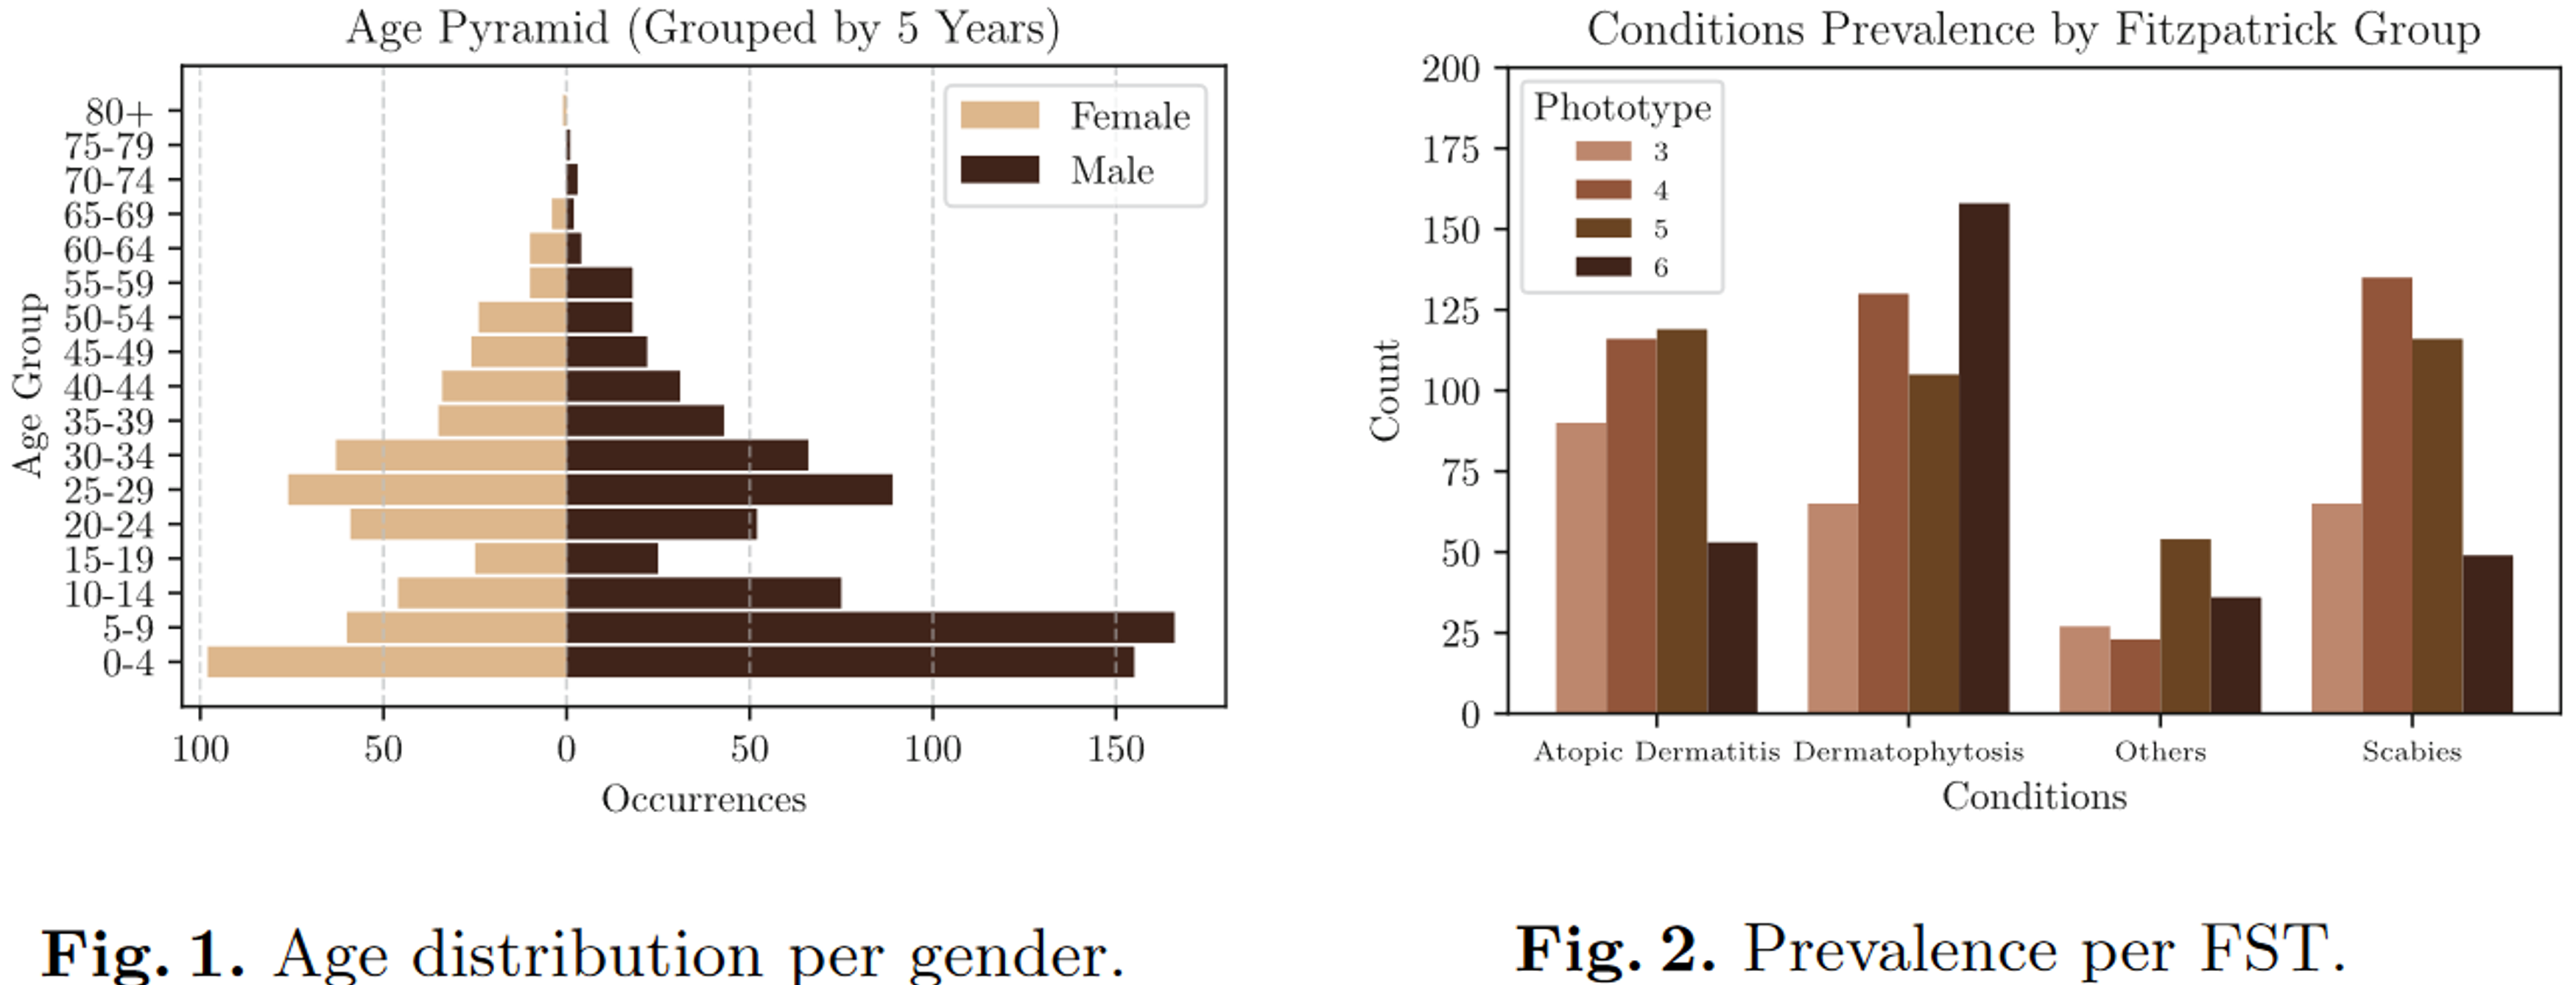
\includegraphics[width=0.9\textwidth]{figures/PASSIONDatasetDistribution.png}
					\caption{PASSION data distributions \autocite{Gottfrois2024}}
					\label{fig:PASSIONDistr}
				\end{figure}
				
				
				Due to the sensitivity of patient data, the dataset is confidential. Access to it can be requested via the project website: \href{https://passionderm.github.io/}{https://passionderm.github.io/} \autocite{Gottfrois2024}.
				
			\subsection{PASSION Model}
			  The model architecture is a ResNet-50 model which is pretrained on ImageNet. The model was fine-tuned by replacing the last fully connected classification layer with a dropout layer with a 0.3 dropout rate followed by batch normalization. The class activation is done by a single linear layer. To minimize the weighted cross-entropy loss, Adam optimization is used. For improved generalization and to avoid overfitting, data augmentations were applied. The methods used were random resizing, cropping, flipping, and rotating. For training, the model uses 5-fold cross-validation \textcite{Gottfrois2024}.
			  			
			\subsection{PASSION Experiments}
			  The PASSION team conducted various experiments to evaluate the classifiers on the test set with the following schemes \autocite{Gottfrois2024}:
			  \begin{itemize}
			  	\item Performance for skin condition prediction
			  	\item Performance for impetigo detection
			  	\item Generalization from two centers to a wider population (test set contains data from the known centers and one unknown center)
			  	\item Generalization from different age groups (test set contains data from the known age groups and one unknown)
			  	\item Subject level analysis over the predictions of multiple images, using majority voting
			  \end{itemize}
			  
			  The code for those experiments is available in the PASSION evaluation GitHub repo. This repo can serve as a starting point, since reproducing the results helps to verify that the provided setup works the same on my side. Also, they can be used as examples for further experiments. \todo{mention which ones I really used why for the thesis and move the others to the appendix}
			  
			  The paper indicates lower performance when evaluating the model on a subject level (performance per case/patient) rather than a sample level (performance per image). The authors emphasize the importance of assessing classifier performance on both levels for completeness \autocite{Gottfrois2024}. Therefore, the subject level performance should also be considered during this thesis.
			  \todo{challenge this to be tested again in the outlook bc of the inproper metadata linkage}
	
	
		\subsection{Limitations}
				\todo{maybe move to execution phase}
				\todo{write in more details}
			   - multiple executions showed inconsistent results for the different group evaluations on the same model checkpoint. It turned out that the metadata linkage did not work consistently. The issue was resolved by providing the image name in the data loader and link the metadata directly from the source file instead of using the indexes. probably related to different shuffling between data loader and metadata loader.
		
			\begin{comment}
		
			
			\end{comment}
		
		\section{Bias}
			This chapter provides an overview of biases and related demographic characteristics mentioned in \gls{ML}- and dermatology-related research. It also explains their relevance for PASSION.
			
			Algorithmic decisions made by \gls{AI} systems can directly affect peoples' lives. In healthcare applications such as PASSION, these decisions are especially sensitive, as they influence diagnoses and treatment outcomes. Diverse studies have shown that \gls{AI} application's decisions can hold biases that affect underrepresented groups. This leads to unfair or even harmful consequences. Therefore, it is essential for \gls{AI} engineers to identify, address, and mitigate such biases in order to develop fair applications. This requires an understanding of what bias is in general, which concrete biases exist, and where they originate \autocite{Mehrabi_2021}.
		
			\subsection{Definition of Bias in \gls{ML}}
		    In the context of \gls{ML}, bias can be defined as \textit{a systematic error that causes a model or estimator to consistently deviate from the true value or relationship} \autocite{Delgado-Rodriguez_2004, Taylor_2023}. In practice, this often results in models that make less accurate predictions for specific subgroups within the population \todo{cite this}.
		    			    
		  	\todo{make sure the following is cited correctly}
			
			\subsection{Demographic Biases in the Context of Dermatology} \label{chap:demographicBiasesDermatology}
			Biases in dermatology in general can lead to unequal outcomes for different groups, which can result in unfair outcomes for certain groups. Demographic biases are particularly relevant in the context of dermatology \glspl{AI}, as they can cause differences in diagnostic accuracy and treatment outcomes among different demographic (sub-)groups.
			From the literature review, three main ways have been identified in which demographic differences may introduce bias in dermatology \gls{ML} models:
			\todo{cite all that, from presentation}
			
			\begin{itemize}
				\item \textbf{Disease Presentation}. \textit{Skin type} affects how diseases appear on the skin. As Gottfrois notes, "any condition linked to inflammation is less visible if the skin is more pigmented" \todo{cite mail from philippe}. This directly influences training and evaluating image-based \gls{ML} models like those used in PASSION. For example, a model trained predominantly on images with low pigmented skin may perform poorly on images of highly pigmented skin.
				
				\item \textbf{Disease Prevalence}. Factors such as \textit{age} and \textit{sex} do not tend to affect disease presentation, but they can influence disease prevalence \todo{cite mail from philippe}. Also, \textit{geographic location} can influence the prevalence of skin conditions (e.g., tropical vs. dry climates) \todo{add source}. Therefore, these factors could introduce bias if certain conditions are underrepresented in the dataset due to demographic imbalances. \todo{consider adding smt like the car driver example here, indicating that it is not necessarily a problem due to the same disease presentation}
				
				\item \textbf{Access to Healthcare}. \textit{Socioeconomic status} or \textit{geographic location} can also introduce bias. Research shows that patients with lower socioeconomic status are often diagnosed at later stages of the disease, which may alter the visual presentation of the disease. If such cases are missing in training data, the model may fail to recognize them, leading to misdiagnosis. \todo{add example for geographic location?}.
			\end{itemize}
			
			
			To build a robust and fair \gls{ML} model, it is essential to identify and address biases linked to such protected characteristics \autocite{Mehrabi_2021}.
			\todo{check that there is no duplication between PASSION dataset feature description and here}
			\todo{probably remove}
			Due to time constraints, this thesis focuses on three protected characteristics: \textit{skin type, age}, and \textit{sex}. These were selected based on their presence in the PASSION dataset and their influence on dermatological diagnosis and disease prevalence. Other potentially relevant features, such as geographic location and socioeconomic status, should be evaluated in future work by the PASSION team.
			
			
			\begin{comment}
				\todo{if citing is an issue: check the comment}
						
				It captures three distinct pathways through which demographic differences can introduce bias in dermatological machine learning systems:
				
				Disease Presentation — covers how diseases manifest differently on various skin types, directly affecting the visual input to image-based models.
				Disease Prevalence — focuses on who is more likely to have certain conditions, which affects label distribution in the dataset.
				Access to Healthcare — reflects when and how people enter the medical system, influencing data collection quality and representativeness.
				
				Each of these groups addresses a different layer of the data generation and learning process:
				
				Input variability (visual features),
				Target/label imbalance (class representation),
				Data collection bias (who gets diagnosed and when).
				
				This structure is also supported in literature on medical \gls{AI} fairness (e.g., in works by Obermeyer et al. or Adamson & Smith).
			\end{comment}
			
			\subsection{Other Types of Biases}
			The literature describes numerous types of bias. Over 50 were identified during this research. These biases were grouped into categories to provide an overview.
			
			\autoref{tab:biases_types} provides an overview of the types of biases identified in the literature. The base categorization follows the main stages of the \gls{ML} lifecycle where the observed bias in the model originated (data collection, algorithm design, and user interaction) as proposed by \textcite{Mehrabi_2021}.
			
			\begin{figure}[H]
				\centering
				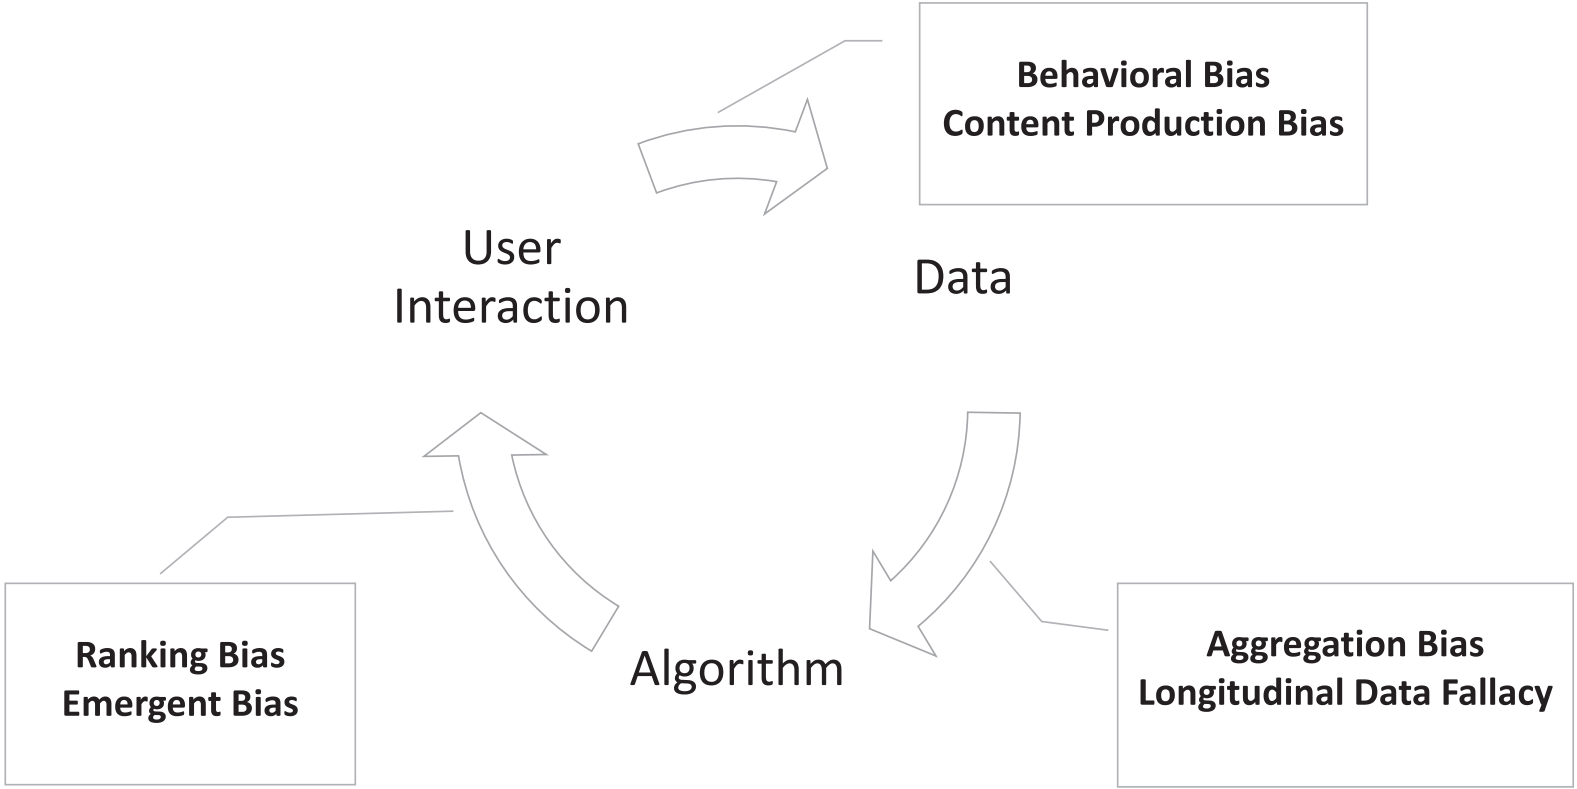
\includegraphics[width=0.8\textwidth]{figures/BiasCategoriesInMLLifecycle.png}
				\caption{\glslink{ML}{ML} lifecycle with fitting biases \autocite{Mehrabi_2021}.}
				\label{fig:bias_definitions_ML_lifecycle}
			\end{figure}
			
			Each specific category groups together similar kinds of biases. Notably, some biases may reasonably fit into multiple categories. Definitions of the categories and the specific biases, can be found in \linkapp{app:listOfBiases}.
			
			\begin{table}[H]
				\centering
				\begin{threeparttable}
					\begin{tabularx}{\textwidth}{>{\tblWidthDescription}X|>{\tblWidthContext}X|>{\tblWidthContext}X}
						\toprule
						\textbf{Bias} & \multicolumn{2}{c}{\textbf{Mentioned in Context of}} \\
						& \textbf{\gls{ML}} & \textbf{Dermatology} \\
						%	\midrule
						\multicolumn{3}{l}{\bolditalic{Data Collection}} \\ 
						
						Sampling Biases & X\tnote{1,2,3} & X\tnote{4} \\
						Representation Biases & X\tnote{1} & X\tnote{5,6} \\
						Measurement Biases & X\tnote{1,3} & X\tnote{4,6} \\
						Research Biases & X\tnote{7} & X\tnote{4} \\
						Feature Representation Biases & X\tnote{1,3} & X\tnote{4} \\
						Imaging Biases & & X\tnote{5} \\
						Medical Biases & X\tnote{8} & X\tnote{4} \\
						Temporal Biases & X\tnote{1} & X\tnote{4}\\
						
						%	\midrule
						\multicolumn{3}{l}{\bolditalic{Algorithmic Design}} \\ 
						Algorithmic Biases & X\tnote{1} & \\
						External Influence Biases & X\tnote{1} & X\tnote{4} \\
						
						%	\midrule
						\multicolumn{3}{l}{\bolditalic{User Biases}} \\
						Cognitive Biases & X\tnote{1,7} & X\tnote{4} \\
						Behavioral Biases & X\tnote{1,3} & X\tnote{4,5} \\
						Publication Biases &  & X\tnote{4} \\
						Medical Biases & X\tnote{} & X\tnote{4} \\
						
						\bottomrule
					\end{tabularx}
					\begin{tablenotes}
						\footnotesize
						\begin{minipage}{0.33\textwidth}\raggedright
							\item[1] \autocite{Mehrabi_2021}
							\item[2] \autocite{HP_2022}
							\item[3] \autocites{Mester_2022}
						\end{minipage}%
						\begin{minipage}{0.33\textwidth}\raggedright
							\item[4] \autocite{Chakraborty_2024}
							\item[5] \autocite{Young_2020}
							\item[6] \autocite{Montoya_2025}
						\end{minipage}%
						\begin{minipage}{0.33\textwidth}\raggedright
							\item[7] \autocites{Mester_2017}
							\item[8] \autocite{Delgado-Rodriguez_2004}
						\end{minipage}%
					\end{tablenotes}
				\end{threeparttable}
				\caption{Bias categories - grouped according the \glsentryshort{ML} lifecycle of \textcite{Mehrabi_2021}}
				\label{tab:biases_types}
			\end{table}
			
			
			\subsection{Sensitive Features}
			Research has identified sensitive features that are particularly prone to bias. These features have already caused biases in existing \gls{AI} applications and should therefore be carefully evaluated during model development \autocite{Mehrabi_2021}.
			
			\autoref{tab:biases_features} summarizes sensitive features mentioned in the literature. The categorization in the table was done based on the research described in \autoref{chap:demographicBiasesDermatology}. For completeness, the table also contains sensitive demographic features which appear unrelated to dermatology according based on current research.
			
			\begin{comment}
			\todo{check what to do with those additional features:}
			Other important features according to (\autocite{Montoya_2025} 13):
			lesion type, anatomical location of lesion, img characteristics such as source, imaging techniques, resolution, real vs. artificially generated
			
			In addition to demographic factors, domain-specific variables such as lesion type, anatomical location, and image characteristics (e.g., imaging technique, resolution, device source, or whether an image is real vs. artificially generated) can also influence model behaviour \autocite{Montoya_2025}. These features are important considerations for dataset curation and model evaluation in dermatology-focused applications like PASSION.
			\end{comment}
			
			
			\begin{table}[H]
				\centering
				\begin{threeparttable}
					\begin{tabularx}{\textwidth}{>{\tblWidthDescription}X|>{\tblWidthContext}X|>{\tblWidthContext}X}
						\toprule
						\textbf{Bias-Sensitive Features} & \multicolumn{2}{c}{\textbf{Mentioned in Context of}} \\
						& \textbf{\gls{ML}} & \textbf{Dermatology} \\
						%\midrule
						\multicolumn{3}{l}{\bolditalic{Related to Disease Presentation}} \\
						Skin Type & X\tnote{1,2,7} & X\tnote{12,13}\\
						Skin Undertones & & X\tnote{13} \\
						Socioeconomic Status & X\tnote{6} & X\tnote{12} \\
						Geographic Location \todo{double check this!} & X\tnote{1,3} & \\
						
						\multicolumn{3}{l}{\bolditalic{Related to Disease Prevalence}} \\
						Age & X\tnote{7,11} &  X\tnote{13} \\
						Gender/Sex & X\tnote{1,2,7,8,9,10,11} & X\tnote{13} \\
						Gender and Skin Type Subgroups & X\tnote{1,2} & \\
						
						\multicolumn{3}{l}{\bolditalic{Related to Access to Healthcare}} \\
						Geographic Location & X\tnote{1,3} & \\
						Socioeconomic Status & X\tnote{6} & X\tnote{12} \\
						
						\multicolumn{3}{l}{\bolditalic{Relation to Dermatology to be Checked}} \\
						Ethnicity/Race & X\tnote{1,2,4,5,6,7,11}&  X\tnote{12,13} \\
						Disabilities & X\tnote{7,11} & \\
						
						\multicolumn{3}{l}{\bolditalic{Unrelated to Dermatology}} \\
						Familial status & X\tnote{7} & \\
						Marital status & X\tnote{7,11} & \\
						Nationality/National origin & X\tnote{7,11} & \\
						Recipient of public assistance & X\tnote{7} & \\
						Religion & X\tnote{7,11} & \\
						\bottomrule
					\end{tabularx}
					\begin{tablenotes}
						\footnotesize
						\begin{minipage}{0.33\textwidth}\raggedright
							\item[1] \autocite{Mehrabi_2021}
							\item[2] \autocite{M24_Buolamwini_2018}
							\item[3] \autocite{M142_Shankar_2017}
							\item[4] \autocite{M98_Manrai_2016}
							\item[5] \autocite{M54_Fry_2017}
						\end{minipage}%
						\begin{minipage}{0.33\textwidth}\raggedright
							\item[6] \autocite{M150_Vickers_2014}
							\item[7] \autocite{M30_Chen_2019}
							\item[8] \autocite{M167_Zhao_2017}
							\item[9] \autocite{M20_Bolukbasi_2016}
							\item[10] \autocite{M168_Zhao_2018}
						\end{minipage}%
						\begin{minipage}{0.33\textwidth}\raggedright
							\item[11] \autocite{M62_Hajian_2013}
							\item[12] \autocite{Young_2020}
							\item[13] \autocite{Montoya_2025}
						\end{minipage}%
					\end{tablenotes}
				\end{threeparttable}
				\caption{Commonly used features which often are affected by biases}
				\label{tab:biases_features}
			\end{table}
			
			
			\begin{comment}
			\todo{decide which table to use, more or less extensive citations?}
			
			\begin{table}[H]
				\centering
				\begin{threeparttable}
					\begin{tabularx}{\textwidth}{>{\tblWidthDescription}X|>{\tblWidthContext}X|>{\tblWidthContext}X}
						\toprule
						\textbf{Bias-Sensitive Features} & \multicolumn{2}{c}{\textbf{Mentioned in Context of}} \\
						& \textbf{\gls{ML}} & \textbf{Dermatology} \\
						%\midrule
						\multicolumn{3}{l}{\textbf{Dermatology Related Features}} \\
						Skin Type & X\tnote{1,3} & X\tnote{5,6}\\
						Skin Undertones & & X\tnote{6} \\
						
						\multicolumn{3}{l}{\textbf{Demographic Features}} \\						\multicolumn{3}{l}{\bolditalic{Relevant for Skin Disease Detection}} \\
						Age & X\tnote{3,4} &  X\tnote{6} \\
						Gender/Sex & X\tnote{1,3,4} & X\tnote{6} \\
						Gender and Skin Type Subgroups & X\tnote{1} & \\
						Ethnicity/Race & X\tnote{1,2,3,4}&  X\tnote{5,6} \\
						
						\multicolumn{3}{l}{\bolditalic{Potentially Relevant for Skin Disease Detection}} \\
						Geographic Location & X\tnote{1} & \\
						Socioeconomic Status & X\tnote{2} & X\tnote{5} \\
						Disabilities & X\tnote{3,4} & \\
						
						\multicolumn{3}{l}{\bolditalic{Not Relevant for Skin Disease Detection}} \\
						Familial status & X\tnote{3} & \\
						Marital status & X\tnote{3,4} & \\
						Nationality/National origin & X\tnote{3,4} & \\
						Recipient of public assistance & X\tnote{3} & \\
						Religion & X\tnote{3,4} & \\
						\bottomrule
					\end{tabularx}
					\begin{tablenotes}
						\footnotesize
						\begin{minipage}{0.30\textwidth}\raggedright
							\item[1] \autocite{Mehrabi_2021}
							\item[2] \autocite{M150_Vickers_2014}
						\end{minipage}%
						\begin{minipage}{0.40\textwidth}\raggedright
							\item[3] \autocite{M30_Chen_2019}
							\item[4] \autocite{M62_Hajian_2013}
						\end{minipage}%
						\begin{minipage}{0.30\textwidth}\raggedright
							\item[5] \autocite{Young_2020}
							\item[6] \autocite{Montoya_2025}
						\end{minipage}%
					\end{tablenotes}
				\end{threeparttable}
				\caption{Features which often hold biases}
				\label{tab:biases_sensitive_features}
			\end{table}
			\end{comment}
			
		\section{Fairness Metrics}
		This chapter introduces the concept of fairness in \gls{ML}, as fairness is a way to detect whether and what biases exist in a model. As there is no universally accepted definition of fairness, various fairness metrics have been proposed in the literature, each based on different assumptions and goals \autocite{Mehrabi_2021}.
		
		
		\subsection{Definition of Fairness in \gls{ML}}
		
		In research, there is currently no common agreement regarding a fairness definition in \gls{ML}. Broadly, fairness \textit{is the absence of bias towards individuals or groups in a decision-making context}. To assess how fair \gls{AI} models are, multiple fairness metrics have been proposed in the literature, each reflecting different interpretations of fairness. The choice of metric largely depends on the specific use case of the application \autocite{Mehrabi_2021}.
		
		\subsection{Fairness Metrics} \label{chap:FairnessMetrics}
		
			\textcite{Mehrabi_2021} summarized the fairness metrics and grouped them into the categories group fairness, subgroup fairness and individual fairness, depending on the main mechanics of the metrics. They are listed in \autoref{tab:fairness_definitions}.
		
			\begin{table}[H]
			\centering
			\begin{threeparttable}
				\begin{tabularx}{\textwidth}{>{\tblWidthDescription}X|>{\tblWidthContext}X|>{\tblWidthContext}X}
					\toprule
					\textbf{Fairness Definitions} & \multicolumn{2}{c}{\textbf{Mentioned in Context of}} \\
					& \textbf{\gls{ML}} & \textbf{Dermatology} \\
					%	\midrule
					\multicolumn{3}{l}{\bolditalic{Group Fairness}} \\ 
					Conditional Statistical Parity    & X &   \\
					Demographic/Statistical Parity  & X & \\
					Equal Opportunity& X &   \\
					Treatment Equality & X &   \\
					Test Fairness         & X &   \\
					Equalized Odds     & X &   \\
					%	\midrule
					\multicolumn{3}{l}{\bolditalic{Subgroup Fairness}} \\ 
					Subgroup Fairness    & X &   \\
					%\midrule
					\multicolumn{3}{l}{\bolditalic{Individual Fairness}} \\ 
					Counterfactual Fairness     & X &   \\
					Fairness Through Awareness     & X &   \\
					Fairness Through Unawareness        & X &   \\
					%\midrule
					\multicolumn{3}{l}{\bolditalic{Not Categorized}} \\ 
					Fairness in Relational Domains& X &   \\
					\bottomrule
				\end{tabularx}
			\end{threeparttable}
			\caption{Fairness definitions based on \textcite{Mehrabi_2021}}
			\label{tab:fairness_definitions}
		\end{table}
		
		To better understand how fairness can be formally defined, consider the example of equalized odds, introduced by \textcite{M63_Hardt_2016}: \newline
		"\textit{A predictor $\hat{Y}$ satisfies equalized odds with respect to protected attribute $A$ and outcome $Y$, if $\hat{Y}$ and $A$ are independent conditional on $Y$. \newline
			\(
			P(\hat{Y} = 1 \mid A = 0, Y = y) = P(\hat{Y} = 1 \mid A = 1, Y = y), \quad \forall y \in \{0, 1\}
			\)"} \todo{add formula list} \newline
		In other words, the probability of predicting a positive outcome should be the same across protected and unprotected groups, given the true label $Y$. This ensures that both \gls{TPR} and \gls{FPR} are equal across different demographic groups. If these rates are the same, like in the example of \autoref{fig:eqOdds}, the model satisfies equalized odds, and fairness is achieved. Since equalized odds compares conditional probability distributions across groups, it is a group fairness metrics.
		
		\begin{figure}[H]
			\centering
			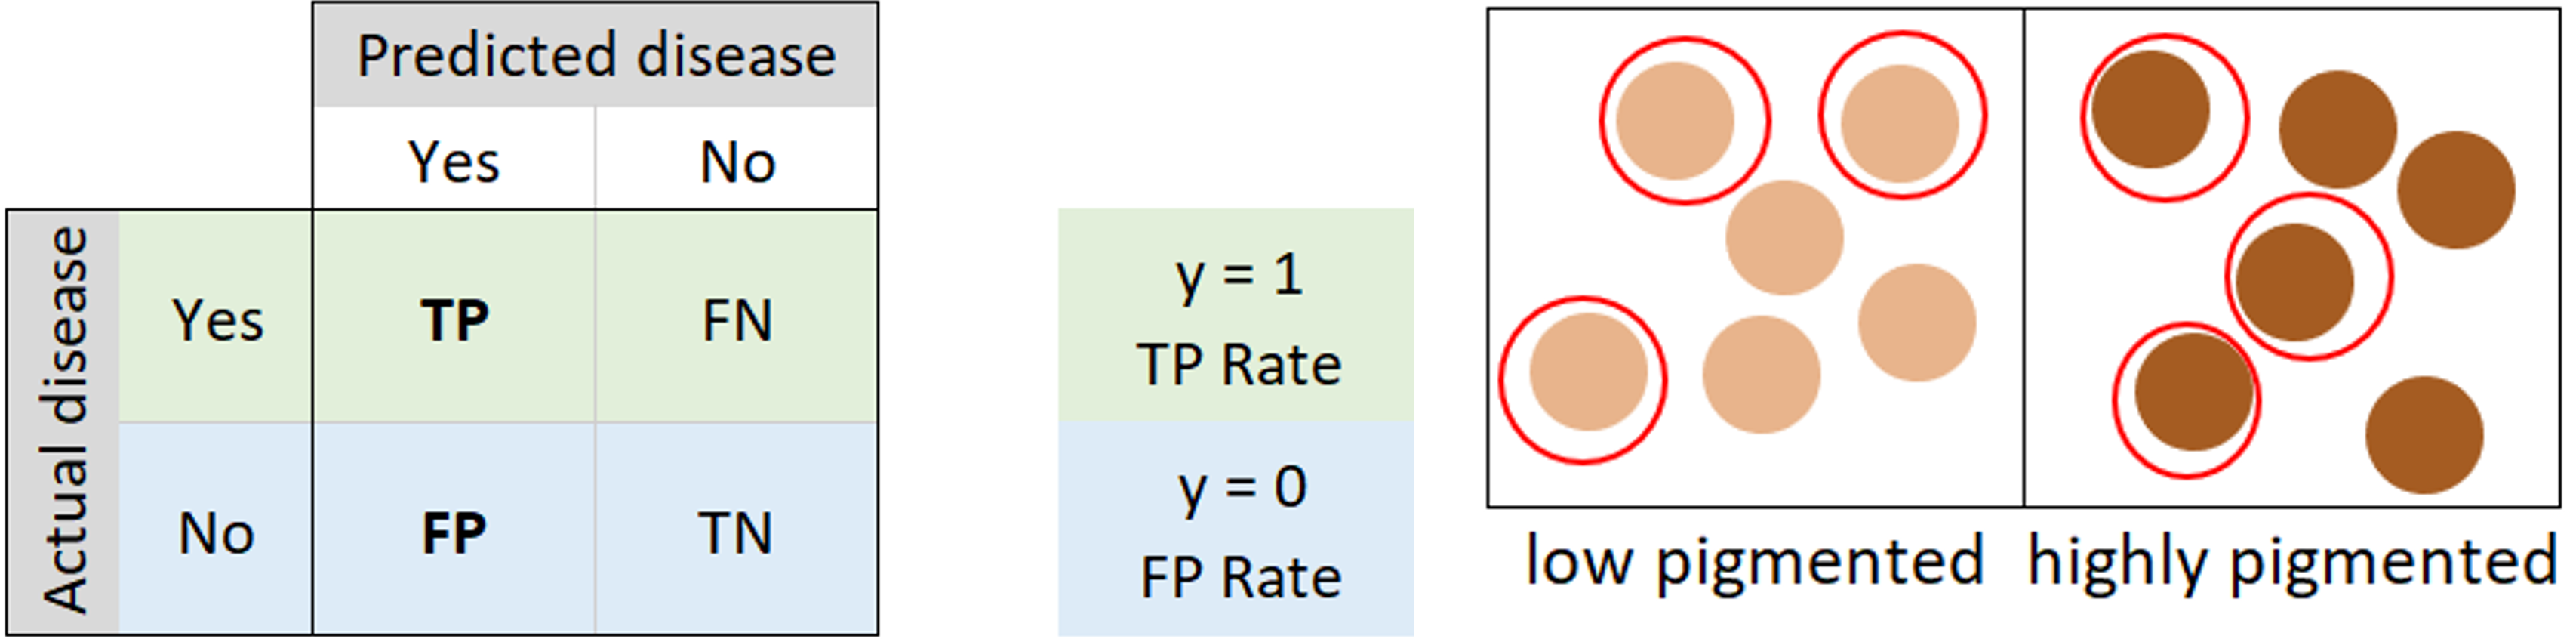
\includegraphics[width=0.9\textwidth]{figures/EqualizedOddsIllustration.png}
			\caption{Equalized odds mechanics, inspired by \textcite{M80_Kearns_2019}.}
			\label{fig:eqOdds}
		\end{figure}
		
		The mechanics of the other fairness metrics are described broadly in \linkapp{app:fairnessMetrics}.
		
		There are Python libraries like \textit{\gls{Fairlearn}} available, which can be used for the computation of the fairness metric \autocite{Agarwal_2018}. They tend to support the most popular metrics for binary classification \autocite{Fairlearn_nodate}.
		
		\subsection{Limitations of Group Fairness}
		
		Despite its usefulness, equalized odds and similar group fairness metrics have limitations. These metrics can hide inequalities that exist within more specific subgroups. For example, a model might appear fair when assessed across broad groups such as age or skin type (\autoref{fig:eqOdds}) but still exhibit substantial disparities within subgroups, such as older individuals with darker skin tones (\autoref{fig:eqOddsLimits}) \autocite{M79_Kearns_2018,M80_Kearns_2019}.
		
		\begin{figure}[H]
			\centering
			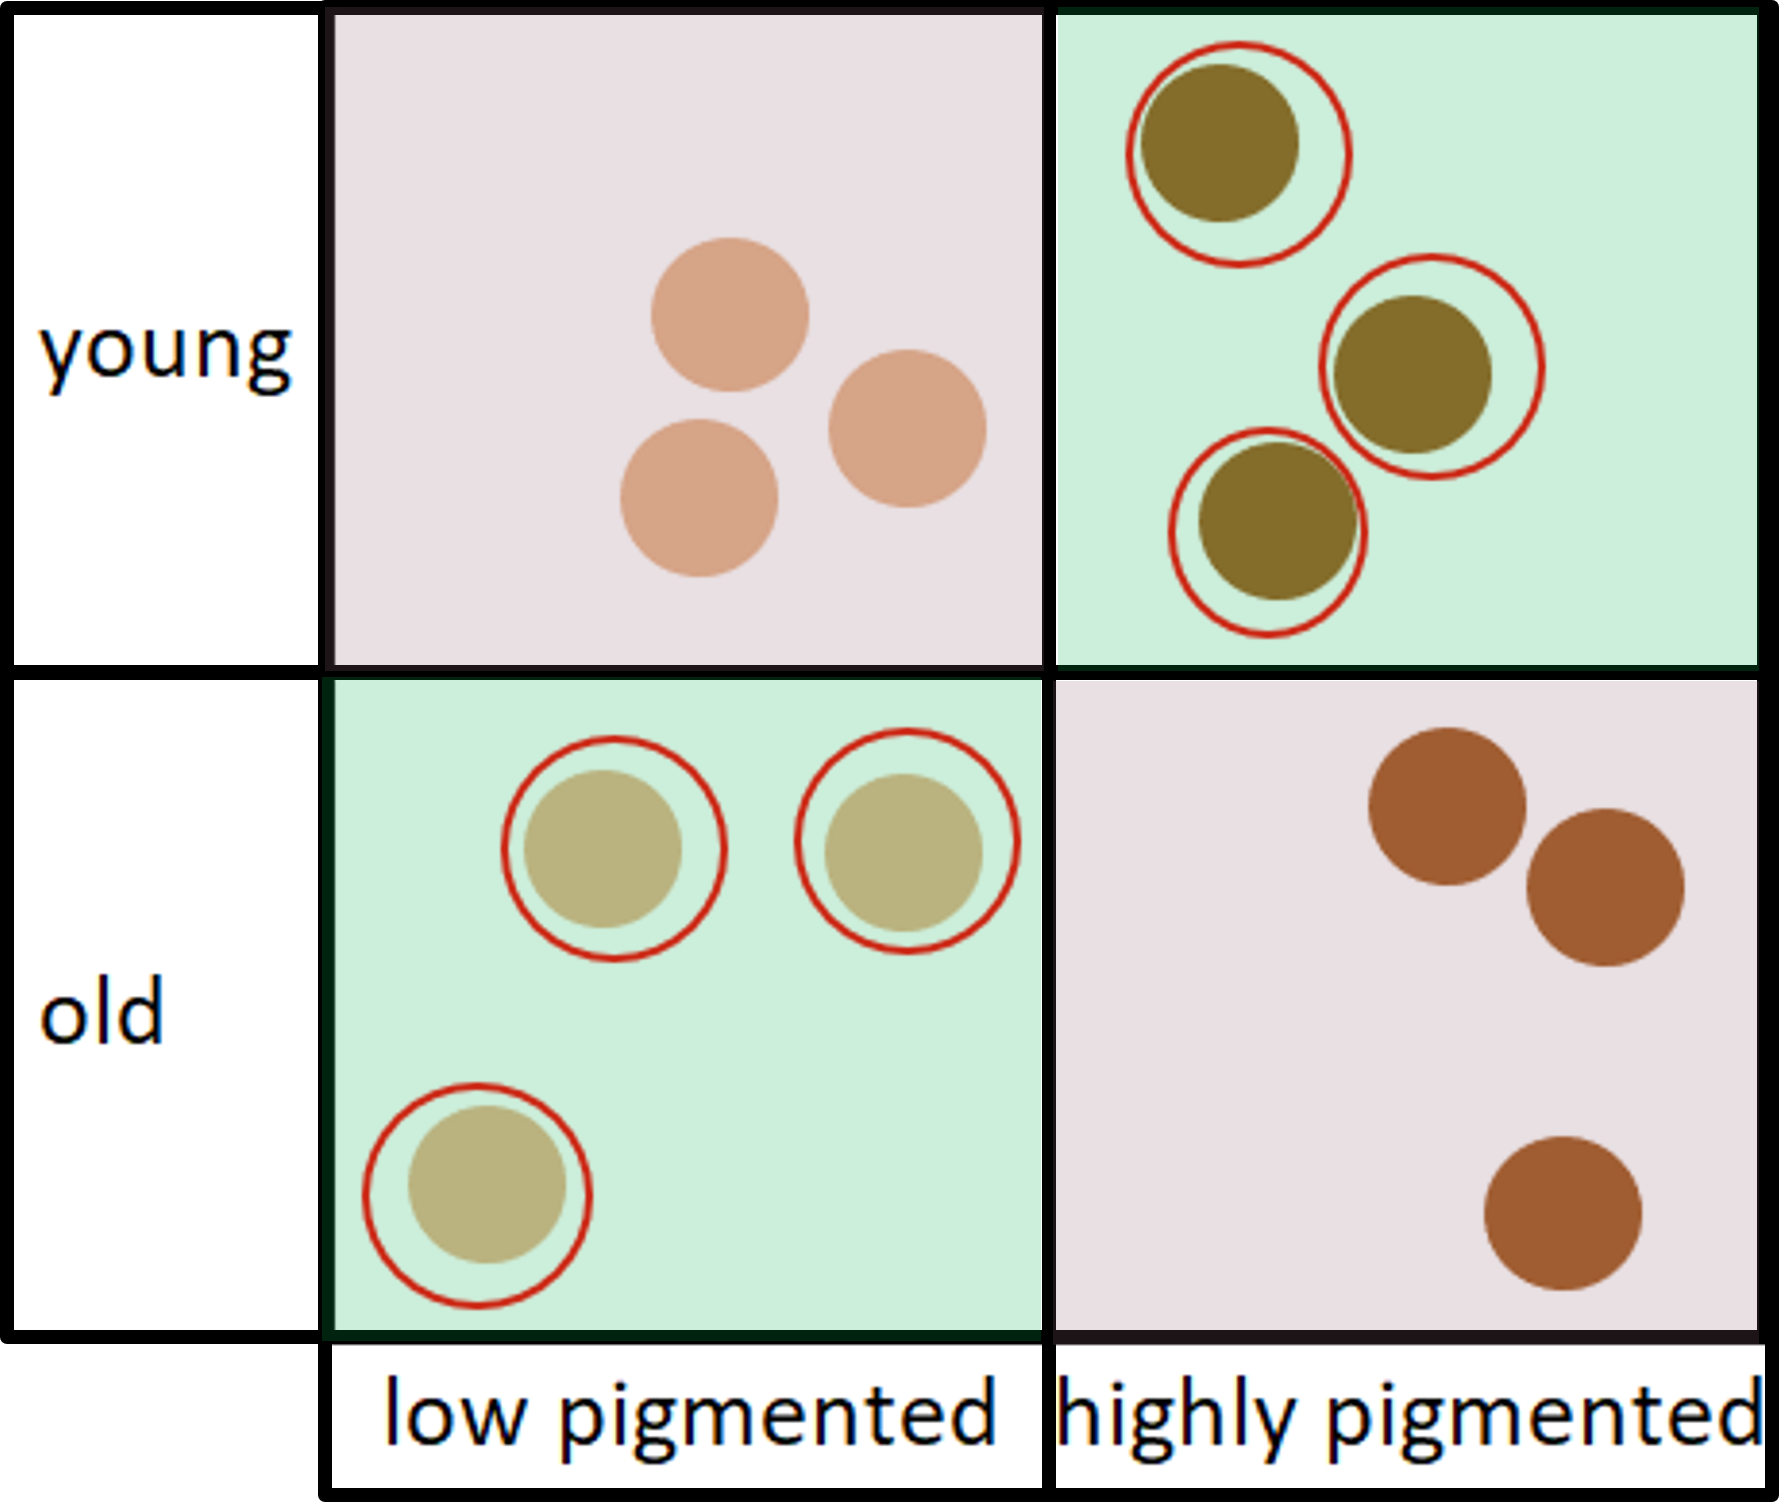
\includegraphics[width=0.5\textwidth]{figures/EqualizedOddsSubgroupsIssueIllustration.png}
			\caption{Equalized odds violations on subgroups, inspired by \textcite{M80_Kearns_2019}.}
			\label{fig:eqOddsLimits}
		\end{figure}
		
		To address this issue, subgroup fairness metrics have been proposed. These extend group fairness metrics by explicitly evaluating fairness across subgroups. This ensures that fairness assessments do not overlook hidden biases that could affect smaller populations \autocite{M79_Kearns_2018,M80_Kearns_2019}.
		
			
		\section{Mitigation Methods} \label{chap:mitigationMethods}
			When biases are identified, they can be reduced through various mitigation methods. Since biases may arise at different stages of the \gls{ML} life cycle, corresponding mitigation strategies exist for each stage. These include e.g., methods for reducing representation disparities in datasets (pre-processing), approaches targeting model architecture and algorithm design (in-processing), and techniques aimed at interpreting model outputs (post-processing) \autocite{Mehrabi_2021}.
			
			This thesis provides an overview of the mitigation methods currently recognized in the field of \gls{ML}, as AI engineers must understand the available methods for reducing bias \autocite{Mehrabi_2021}. \autoref{tab:mitigation_methods_categories} presents a broad categorization of these methods. The focus lies on approaches related to fair data collection and design, as well as fair classification, given the nature of the \gls{ML} task at hand. Specific examples for each category are listed in \autoref{app:mitigationMethods}; for further details, the original sources should be consulted.
			
			\begin{table}[H]
				\centering
				\begin{threeparttable}
					\begin{tabularx}{\textwidth}{>{\tblWidthDescription}X|>{\tblWidthContext}X|>{\tblWidthContext}X}
						\toprule
						\textbf{Mitigation Method Categories} & \multicolumn{2}{c}{\textbf{Mentioned in Context of}} \\
						& \textbf{\gls{ML}} & \textbf{Dermatology} \\
						\multicolumn{3}{l}{\bolditalic{Fair Data Collection and Design}} \\
						Documentation and Transparency & X\tnote{1} & X\tnote{3} \\
						Bias Detection and Evaluation & X\tnote{1} & X\tnote{2,4} \\ % simpsons paradoxon, subset scanning, input pertubation
						Study Design & X\tnote{1} & X\tnote{2} \\ % allocation concealment and blinding, preventing direct and indirect discrimination
						Data Gathering & X\tnote{1} & X\tnote{3,4} \\ % data collection from diverse sources, robuster standards, 
						Removing Sensitive Attributes & X\tnote{1} &  \\
						\multicolumn{3}{l}{\bolditalic{Fair Classification}} \\
						Satisfy Fairness Definitions & X\tnote{1} &  \\ % satisfy Equalized Odds / Subgroup fairness
						Algorithmic Adaptions for Fairness & X\tnote{1} & \\
						Fair Representation Learning & X\tnote{1} & \\
						Fairness-Aware \gls{ML} Frameworks & X\tnote{1} & \\
						Preferential Data Selection and Representation & X\tnote{1} & \\
						Model Interpretability & X\tnote{1} & X\tnote{3} \\
						\multicolumn{3}{l}{\bolditalic{For Other \gls{ML} Tasks}} \\
						Fair NLP & X\tnote{1} &  \\
						Fair Regression & X\tnote{1} &  \\
						Structured Prediction & X\tnote{1} &  \\
						Fair Principal Component Analysis & X\tnote{1} &  \\
						Graph-Based Fairness Methods & X\tnote{1} &  \\
						Causal Fairness and Disparate Learning & X\tnote{1} &  \\
						\bottomrule
					\end{tabularx}
					\begin{tablenotes}
						\footnotesize
						\begin{minipage}{0.33\textwidth}\raggedright
							\item[1] \autocite{Mehrabi_2021}
							\item[2] \autocite{Chakraborty_2024}
						\end{minipage}%
						\begin{minipage}{0.33\textwidth}\raggedright
							\item[3] \autocite{Young_2020}
						\end{minipage}%
						\begin{minipage}{0.33\textwidth}\raggedright
							\item[4] \autocite{Montoya_2025}
						\end{minipage}%
					\end{tablenotes}
				\end{threeparttable}
				\caption{Mitigation method categories}
				\label{tab:mitigation_methods_categories}
			\end{table}
	
	\chapter{Ideas and Concepts}
		This chapter outlines initial thoughts and conceptual considerations for addressing potential biases in the PASSION project. It sketches the general methodology used in this thesis.
		
		\section{Broad Methodology}
			The evaluation and mitigation of bias in the PASSION model is planned to consist of four stages:
			\begin{enumerate}
				\item \textbf{Literature Review.} A literature review will be conducted to get an overview of what biases, fairness metrics, and mitigation strategies are known in medical \gls{AI}.
				
				\item \textbf{Contextualization and Scope Definition.} The findings' relevance for PASSION's \gls{teledermatology} context will be evaluated. Based on this, relevant types of bias, applicable fairness metrics and mitigation methods will be selected. Aspects not feasible to address within the scope of this thesis will be documented for future work.
				
				\item \textbf{Baseline Fairness Assessment.} The current PASSION model will be evaluated using the selected fairness metrics. This will provide a baseline for comparison after mitigation methods are applied.
				
				\item \textbf{Mitigation and Evaluation.} Selected mitigation strategies will be implementend individually. Their effect on model fairness and performance will be assessed relative to the baseline.
			\end{enumerate}
		
		\section{PASSION Dataset Assessment}
			In order to determine the scope and feasibility of the findings in the literature review, the dataset must be assessed.
			The PASSION dataset was created to improve the representation of highly pigmented skin, which is underrepresented in many traditional dermatology datasets. Nevertheless, it may still lack adequate representation of specific subgroups. Such gaps in representativeness could potentially lead to biased model outputs. However, as \textcite{Mehrabi_2021} states, this is not necessarily the case. Therefore, a detailed assessment of representativeness can be postponed until the model output indeed proofs to be biased.
			
			Furthermore, the available metadata determines which biases can be identified and what mitigation methods are possible. E.g., if metadata on age is missing, fairness with respect to age cannot be assessed.
			
			Therefore, the dataset will be reviewed regarding:
			\begin{itemize}
				\item Representation of the main groups to get a first impression
				\item Representation of relevant subgroups if the model output proves to be biased
				\item Completeness of metadata relevant for fairness evaluation
				\item Presence of \glspl{proxyVar} that might complicate fairness assessments
			\end{itemize}
			
			These aspects will help determine the extent to which the dataset supports meaningful fairness analysis and subgroup-level model evaluation. It also provides guidance on how to potentially adapt the dataset in the future.
		
			
%		\begin{comment}
%			\section{some general mitigation method ideas}
%				\todo{add infos from the midterm presentation}
%			
%				\todo{write things to consider more precisely:}
%				\begin{itemize}
%					\item Divide and Conquer vs. All-In-One-Model
%					\begin{itemize}
%						 \item An algorithm per ethnicity / subgroup running at the same time
%						\item Running 1 Algorithm chosen based on Fitzpatrick skin type
%						\item Running 1 Algorithm which detects first the demographic subgroup (\gls{FST}, gender, age, …) and runs the specific subgroup algorithm afterwards
%						\item Hint Ludovic: Still not of data, maybe also others; often limited because the data is missing, you are missing data from others
%					\end{itemize}
%					\item BLIND performance vs. Including the demographic data
%					\begin{itemize}
%						\item Idea to try if the labels are not relevant for the diagnosis and should only be used for evaluating fairness purposes as some papers suggest 
%						\item Might be obsolete after demographic biases in dermatology research, since melanin response and melanoma risk is different in male and female according to research https://pmc.ncbi.nlm.nih.gov/articles/PMC4797181/
%					\end{itemize}
%					\item Hint Ludovic: Maybe Focal Loss more relevant --> emphasis on data vs. model
%				\end{itemize}
%				\begin{itemize}
%					\item Divide and Conquer vs. All-In-One-Model (either by etnicity x algorithms at a time or one which seperates the imgs first by demographic subgroup (incl. Fitzpatrick skin type))
%					\item BLIND performance vs. Including the demographic data
%				\end{itemize}
%		
%		\end{comment}	
	\chapter{Methods}\label{chap:methodology}
		This chapter describes the methodological approach and project organization used in this thesis. It outlines the selected process model, planned research methods, and relevant conditions. The focus lies on ensuring that the chosen methods are appropriate, transparent, and justified in the context of evaluating and mitigating bias in the PASSION project.
		
		\section{Project Management}
		This chapter illustrates the process model used, how the progress and risk are managed, and the technical constraints available. This gives an overview of the constraints and the general plan of this thesis. 
		
		\subsection{Process Model}
		The project follows the waterfall model. This means the tasks are completed sequentially and each sequence is based on the one before \autocite{Petersen_2009}. This model has been chosen for the project, since it provides a solid base while keeping the project management overhead small.
		This project is separated into two phases:
		
		\textbf{Phase 1 – Literature Review and Methodology Planning.} This phase includes the literature review, the selection and justification of fairness metrics and bias mitigation techniques, and the assessment of the dataset's structure and limitations. Based on these results, a detailed plan for the second phase is developed.
		
		\textbf{Phase 2 – Execution and Evaluation.} In the second phase, the planned assessments and mitigation strategies are implemented. The PASSION model is evaluated against the selected fairness metrics, and improvements are measured and discussed.
		
		The detailed project plan is included in the provided zip-file.
		
		\subsection{Progress Monitoring and Risk Management}
		To ensure project transparency and timely delivery, bi-weekly status meetings with the advisor are scheduled. Each meeting is prepared beforehand. Discussed are:
		\begin{itemize}
			\item Work completed in the last period
			\item Planned work for the next period
			\item Current project status and comparison with planned schedule
			\item Top three project risks and planned mitigation strategies
		\end{itemize}
		
		Meeting protocols, including the risk reports, are included in the appendix. \todo{add to appendix}
		
		\subsection{Technical Constraints}
		Model training is performed on \gls{HSLU}'s \gls{gpuhub} infrastructure, while code development is carried out on a personal notebook. The code is written in Python and based on the existing PASSION project architecture.
		The code base for this thesis is a fork of the PASSION GitHub Project.
		\begin{itemize}
			\item Original Project: \href{https://github.com/Digital-Dermatology/PASSION-Evaluation}{https://github.com/Digital-Dermatology/PASSION-Evaluation}
			\item Fork: \href{https://github.com/teshi24/PASSION-Bias-Evaluation}{https://github.com/teshi24/PASSION-Bias-Evaluation}
		\end{itemize}
		
		
		\section{Literature Review}
		The literature review targets known bias types, fairness metrics, and mitigation techniques in medical \gls{AI}, with special attention to \gls{teledermatology} and demographic factors. Sources include scientific publications, surveys, and technical documentation of relevant libraries. The goal is to build a conceptual and methodological foundation for subsequent analysis.
		
		To ensure the thesis follows scientific standards while still being feasible, the literature review is conducted based on the pragmatic method of \textcite{Alake_2021} as suggested by my advisor. First, the focus is on survey and taxonomy papers, which provide an overview of existing research. Then, more detailed papers on dermatology \gls{AI} are conducted to gain further insight into the healthcare context. Such a 2-step approach has also been done by \textcite{Chen_2024}. In general, the papers are filtered by focusing on title, abstract and conclusion. Only relevant papers are read in full. \todo{cite protocol in appendix, week1}
		
		\section{Contextualization and Scope Definition} \label{chap:contextMethod}
		The relevance of the literature findings is evaluated within the context of the PASSION project. This involves analyzing the findings from the literature review in terms of their relevance to \gls{teledermatology} and similar healthcare applications. This analysis considers the available metadata in the PASSION dataset. Limitations due to dataset constraints or the available time are documented for future work.
		
		The relevance will be categorized into the following groups:
		\begin{itemize}
			\item \textbf{High.} Directly applicable to PASSION, both in terms of the \gls{teledermatology} setting and available metadata; likely to provide valuable insights or improvements. Also, crucial demographic biases are included as high, since PASSION's aim is to create more accessible \gls{AI} models.
			\item \textbf{Medium.} Generally relevant to diagnostic \gls{AI} and PASSION, but do not seem to have the biggest impact towards PASSION's primary goals.
			\item \textbf{Low.} Related to PASSION but only limited. E.g., in the far future it could potentially impact PASSION.
			\item \textbf{Not Applicable.} Not relevant for PASSION due to fundamental differences in domain, type of data, or type of model. For this categorization, no mitigation methods are listed.
		\end{itemize}
		
		Based on this contextual analysis, the highly relevant bias types and mitigation methods are investigated further using the most relevant fairness metrics. The selection process follows domain-specific requirements identified in the literature. Such considerations guide the identification of suitable metrics, which are then justified and evaluated in detail during the execution phase.
		
		To test the fairness assessment which will be implemented, a mitigation method is selected that could feasibly be implemented within the given timeframe. The selection excluded any approaches requiring new data collection and focused on techniques applicable to the existing dataset and resources due to the time limit of this thesis.
		
		This contextual analysis is important, as the context and application of fairness metrics and as well as the effect and therefore importance of potential biases can vary by the use case of the \gls{AI} application \autocite{Mehrabi_2021,Barr_2025}.
		
		\section{PASSION Dataset Assessment}\label{chap:datasetAssessmentMethod}
		The assessment of the PASSION dataset focuses on four core areas:
		
		\begin{itemize}
			\item \textbf{Metadata Completeness.} The metadata is reviewed to verify that all relevant demographic attributes, as identified in the contextualized literature review, are included. Missing attributes limit bias detection and mitigation strategies. They should be added to enable a thorough fairness analysis and bias mitigation. Therefore, potentially missing attributes are listed and passed on to the PASSION team for inclusion in the metadata.
			
			Further, the available sensitive attributes are identified to ensure that they are included in the subgroup fairness evaluation.
			
			\item \textbf{Presence of \glslink{proxyVar}{Proxy Variables}.} Available metadata attributes are assessed regarding their intended purpose and potential use as \glspl{proxyVar}. If \glspl{proxyVar} are identified, alternatives are proposed to be added to the data instead. This step is essential, as relying on \glspl{proxyVar} may introduce unintended bias into the analysis or model.
			
			\item \textbf{Representation of Main Groups.} To evaluate overall demographic distributions, the proportions of the values for each demographic attribute (age, sex, \gls{FST}) are analyzed to identify over- or underrepresented groups. This provides an initial indication of potential data skews, which then can be compared to the model's fairness assessment results. This grants first insight into whether potential unfairness stems from representation bias or other factors.
			
			\item \textbf{Representation of Relevant Subgroups.}
			If the fairness assessment of model outputs reveals unfairness on subgroup levels, the distribution of the subgroups is examined using the same method as for the main groups. As this is a more detailed analysis than the representation of main groups, it is done later in the process if biases regarding subgroups in the model indeed exist.
		\end{itemize}
		\todo{cite methods}
		
		\section{Reproducing PASSION Results}
		Before starting any evaluation on the model, the PASSION experiments must be reproduced on the \gls{gpuhub}, to ensure, that the code base and the data loading is working the same way as for the initial paper. Only then, the evaluation outcome can be used by the PASSION team.
		
				
		\section{Fairness Assessment}\label{chap:fairnessAssessmentMethod}
		To establish a reproducible foundation for fairness evaluations within the PASSION project, a baseline fairness assessment is conducted using the original project setup. The fairness metric selected in \autoref{chap:ContextFairnessMetrics} is implemented in a fairness assessment pipeline to analyze model performance across sensitive subgroups, to identify any potential biases in the model output.
		
		The same fairness assessment process is used to evaluate fairness on the model after applying each mitigation method. This ensures consistency and comparability of results across all experimental stages. A mitigation method is considered to hold potential if it significantly improves the fairness assessment results compared to the established baseline.
		
		The fairness is assessed on a subgroup level. The \gls{Fairlearn} library is used whenever possible to rely on standard implementations. Since \gls{Fairlearn} does not support multiclass analysis and multiple subgroup combinations out of the box, custom code must be developed to handle that part.
		The subgroups are defined by all unique combinations of the sensitive PASSION metadata attributes as evaluated using the method in \linkchap{chap:datasetAssessmentMethod}.
		
		The assessment is run based on the prediction outputs and linked metadata generated in the model evaluation phase, which are cached for later inspection. An independent evaluation class computes the required statistics, and reports fairness metrics. This implementation allows evaluation to be performed independently of model training and supports reproducibility of results.
		
		Alongside with \gls{Fairlearn}, the implementation builds upon \textit{pandas} and \textit{numpy} for data handling, and \textit{scikit-learn} for standard evaluation metrics.
		
		\subsection{Limitations}
			This method provides an initial understanding of fairness in the model output and potential mitigation impacts. However, for scientifically robust conclusions on the fairness impact of a mitigation method, more systematical testing is required.
			
			Ideally, multiple training and evaluation runs per mitigation method using different random seeds should be conducted. Also, the baseline assessment should be run multiple times, using the same seeds to ensure comparison. This approach ensures statistically significant results and accounts for variance due to randomization at diverse stages in the model training process. For instance, \textcite{Valentim_2019} ran each configuration 30 times using different random seeds.
			
			Due to technical limitations and time constraints, multiple runs were not feasible during this thesis. It is strongly recommended that the PASSION team executes the experiments with additional seeds using the provided scripts, to get a more established result.
		
		\section{Mitigation Method Evaluation} \label{chap:mitigationMethodsApplyMethod}
		The PASSION model uses a predefined train-test split. To prevent test set leakage and overfitting while applying mitigation methods, the training data is further divided into a training and a validation set. 
		
		If a mitigation method can be applied in multiple ways (e.g., with different parameters, configurations, or data splits), all these variants are evaluated using the train-validation split to prevent test data leakage. The training for all variants will be done without 5-fold cross-validation which allows for significantly faster iteration cycles. This is crucial given the time limitation for this thesis. The variant that performs best on the validation set is then used to evaluate the effectiveness of the mitigation method on the original test set. For this final assessment, 5-fold cross-validation, as setup by \textcite{Gottfrois2024}, is used again.
		
		This approach ensures that the final test results are comparable across different methods, while keeping the selection process short and independent of the test data.\todo{cite AI lectures}
		\begin{comment}
			AI lectures or textbook, e.g., Goodfellow et al., 2016
			Goodfellow, I., Bengio, Y., Courville, A. (2016). Deep Learning. MIT Press.
			Or a standard practice guideline like:
			Varma, S., Simon, R. (2006). Bias in error estimation when using cross-validation for model selection. BMC Bioinformatics, 7(1), 91.
		\end{comment}
		
		Selected bias mitigation strategies are applied to this setup individually, so that the impact on the fairness can be clearly assigned to the tested mitigation strategy. The impact is evaluated relative to the established baseline as described in \linkchap{chap:fairnessAssessmentMethod}.
		
		To get insight on how the mitigation method influences model performance, also the performance should be compared to the baseline.
		
		\section{Stratified Split Experiment}
		Stratified splitting is a bias mitigation method commonly applied using the target labels to ensure a balanced representation of classes. However, additional attributes can also be included to maintain minority subgroup representation across train and test sets \autocite{Balde_2023}.
		
		This experiment investigates how different stratification strategies affect model fairness. While the PASSION dataset includes a predefined training-test split, the stratification criteria used are undocumented. To approximate the original criteria, the distribution of key attributes is analyzed across the original train and test sets, to get a better understanding of the baseline used.
		
		To maintain comparability with the baseline, the original test set is preserved. The training set is re-split using various stratification configurations. All splits include the target labels, and additional attributes based on known representation disparities are incorporated. A purely random split serves as a control configuration.
		
		Splits are generated using \texttt{sklearn.model\_selection.train\_test\_split} with the \texttt{stratify} parameter. The general evaluation follows the procedure described in \autoref{chap:mitigationMethodsApplyMethod}.
		
	\chapter{Execution}
		\section{Contextualization and Scope Definition}
		This section applies the information found during the literature review to the PASSION project using the method described in \autoref{chap:contextMethod}. It also scopes what information can be assessed during this thesis and what should be passed on to the PASSION team.
		
		\subsection{Bias}
		The categorization of biases in \autoref{app:listOfBiases} has been enhanced by indicating how relevant they are to the PASSION context. Also, mitigation strategies mentioned in the research and based on the contextualization have been added.
		
		Among the categories, \textit{sampling biases} and \textit{representation biases} are particularly \mbox{relevant}, as they relate directly to the inclusion or exclusion of demographic subgroups in the dataset. For example, \textit{ascertainment bias}, a subtype of sampling bias, occurs when parts of the target population are unintentionally excluded. A common example is healthcare studies conducted in public hospitals only, which excludes patients from higher socioeconomic backgrounds who visit private clinics. This skews the data and can lead to incorrect conclusions, such as overestimating disease prevalence in specific groups.
		
		Other relevant categories include \textit{medical biases} and \textit{imaging biases}, especially in the teledermatology setting of PASSION. These include clinical labeling errors, variations in image quality or lighting conditions which lead to bias.
		
		Here, the most interesting biases in regards of PASSION are highlighted. An extensive list of the identified types of bias is provided in \linkapp{app:listOfBiases} and will be shared with the PASSION team for further evaluation. \autoref{app:listOfBiases} also provides some further insight into potentially mitigating the following biases.
		
		For completeness, it is also notable that certain biases can be used to improve \gls{AI} models or the surrounding research. E.g., the \textit{Hawthrone bias} as explained in \autoref{app:HawthroneBias} could improve a projects quality by introducing monitoring via 4-eyes reviews of code or the data annotating process.
		
		
		\paragraph{Annotator Bias}
		This bias is a form of observer bias where human annotators are influenced by personal background, expectations, or external factors, which can lead to inconsistent or skewed labeling of data \autocite{Montoya_2025}. In PASSION, annotator bias could particularly affect the labeling of skin tones, which are somewhat dependent on individual perception. This bias could further lead to inconsistent classifications of skin conditions across different demographic groups. 
		
		\paragraph{Aggregation Bias}
		This bias occurs when conclusions drawn from the entire population do not apply to individual subgroups, leading to incorrect or generalized assumptions. This bias arises when significant differences between subgroups (such as sex or ethnicity) are not properly accounted for \autocite{Mehrabi_2021,M144_Suresh_2021}. Aggregation bias is a significant concern in PASSION, since it involves multiple sensitive demographic factors which impact skin disease prevalence and appearance. The model needs to account for these factors to avoid generalized conclusions that might harm certain subgroups.
		
		\paragraph{Image Quality Bias}
		This bias occurs when the quality of an image, such as the zoom level, focus, lighting, or even different hardware affects how a \gls{ML} model classifies or diagnoses the image. Poor image quality can lead to misclassification or lower prediction accuracy \autocite{Young_2020}. Since PASSION will be used in a \gls{teledermatology} context, it will not be feasible to fully standardize image acquisition which was also proposed by \textcite{Young_2020}. The image quality assessment proposed above is probably the best method going forward. Also, the biased outcome regarding the countries could be an indicator, that this bias indeed exists in PASSION. \textit{Visual artifacts bias} is a related bias which occures based on e.g., the presence of hair in the data and also could be influenced by the data gathering process.
		
		\paragraph{Previous Opinion Bias}
		When the knowledge of prior results or diagnoses influences the interpretation of new data, leading to biased conclusions \autocite{Chakraborty_2024}. This is not only relevant to PASSION's labeling process but even more importantly, it also affect real-world diagnoses once PASSION is deployed. For example, if both the patient and the dermatologist are aware of the model's prediction before the dermatologist evaluates the case, the model's output could influence the final diagnosis. Therefore, it is crucial that the model’s prediction is not shown to users - at least not during triage and prior to the clinical assessment - unless it concerns a condition that users can safely treat themselves.
		
		\paragraph{Diagnostic Access Bias}
		Diagnostic access bias occurs when individuals in certain geographical locations have better access to medical care, leading to earlier diagnosis and potentially higher disease prevalence in those regions \autocite{Chakraborty_2024}. PASSION addresses diagnostic access bias in dermatology \glspl{AI} regarding Sub-Saharan Africa. However, the bias could still be relevant in the dataset, depending on which clinics were chosen for data selection.
		
		
		\subsection{Sensitive Features}
			Some of the listed features in \autoref{tab:biases_features} were also mentioned in the dermatology context and/or are included as metadata in the PASSION dataset. Therefore, potential biases associated with them should be evaluated in the PASSION model.
			
			Since PASSION aims to improve classification of skin diseases based solely on image data without any metadata, it does not use these factors as features for training, except for characteristics that are implicitly visible in the images. This is primarily the \textit{skin type} (including the undertone). More broadly defined, the \textit{socioeconomic status} and \textit{geographic location} can also be leaked to the model through the images, due to their impact on disease presentation and progression. Since the model can access these characteristics during training, they can introduce bias and should therefore be closely examined.
			
			\textit{Age} and \textit{sex} are generally not visible in the images. Also, \textit{socioeconomic status} and \textit{geographic location} do not necessarily need to lead to visual effects. However, since they can influence disease prevalence and are prone to bias, the PASSION model should be evaluated for potential bias regarding these characteristics.
			
			The potential impact of \textit{ethnicity} and \textit{disabilities} on visual presentation or prevalence of dermatological conditions has not been assessed in this thesis, due to time constraints. It is recommended that the PASSION team investigates these aspects further.
			
			The other sensitive features do not seem to be further relevant for PASSION.
		
		\subsection{Fairness Metrics} \label{chap:ContextFairnessMetrics}
		This chapter focuses on those fairness metrics which can evaluate demographic fairness and are applicable to the dermatology context of PASSION.	Those are mainly \textit{equalized odds} by \textcite{M63_Hardt_2016} and \textit{subgroup fairness} by \textcite{M79_Kearns_2018}.
		
		In the context of PASSION, fairness metrics which consider both \textit{true positives} and \textit{false positives} are particularly relevant. A true positive indicates that a disease was detected correctly, while a false positive corresponds to a diagnosis of a disease that is not actually present. Including false positives helps to identify cases where individuals from certain demographic groups may be unfairly more likely to receive unjustified diagnoses. This has also been indicated by \textcite{Sabato_2024}.
		
		From the listed group fairness metrics in \autoref{tab:fairness_definitions}, only equalized odds considers true and false positives, which should therefore be used for the evaluation of PASSION. A detailed explanation of equalized odds is provided in \autoref{chap:FairnessMetrics}.
		
		Given the specific dermatology use case in the context of PASSION, it is not clear whether individual fairness metrics would be feasible to use. Certain metrics propose to change attributes. This approach is not feasible for the skin type which is passed on to the model implicitly through the image. Therefore, this thesis focuses on the group fairness metrics for now.
		
		Given the demographic focus of this study and the composition of the PASSION dataset, subgroup fairness is particularly important. Therefore, this thesis aims to incorporate equalized odds on subgroups as a core metric for evaluation.
		
		\paragraph{Limitations of Fairness Evaluation with Equalized Odds for PASSION}
		Fairness metrics such as equalized odds are originally defined for binary classification problems, typically considering binary labels and binary demographic groups. As a result, fairness libraries like \gls{Fairlearn} offer implementations of these fairness metrics only for binary classification tasks \autocite{Fairlearn_nodate}. To evaluate fairness in multiclass settings using these libraries, certain considerations are required. This chapter introduces the two key challenges for the fairness evaluation of PASSION, handling multiclass labels and multiple subgroups.
		
		\subparagraph{Multiclass Labels}
		In binary settings, fairness can be evaluated through simple comparisons of false positive and false negative rates. However, in multiclass classification, fairness must account for the full structure of the confusion matrix. \textcite{Sabato_2024} generalizes equalized odds to multiclass classification by defining:
		\textit{"For each \( y, z \in \mathcal{Y} \), the value of \( \mathbb{P}[\hat{Y} = z \mid Y = y, G = g] \) is the same for all \( g \in \mathcal{G} \)."}
		
		In practice, this means the entire confusion matrix must be equal across groups to satisfy strict multiclass fairness under equalized odds \autocite{Sabato_2024}. A similar approach is proposed by \textcite{Putzel_2022}.
		
		More relaxed versions of multiclass equalized odds have also been proposed in the literature, such as applying equalized odds per class. However, researchers argue that such relaxations may not be suitable in all contexts, especially when different types of errors carry different consequences \autocites{Sabato_2024}{Putzel_2022}.
		
		For instance, when the type of misclassification matters, equality of error rates is essential to ensure fairness, as noted by \textcite{Putzel_2022}. Furthermore, as \textcite{Sabato_2024} explicitly states, a fair classifier in healthcare should avoid differences in diagnosis errors for specific diseases across subgroups, since misdiagnoses can lead to different treatment outcomes.
		
		Therefore, in PASSION, the strict version of the multiclass equalized odds should be preferred. However, the code provided by \textcite{Sabato_2024} was not easy reusable, and there is no such version included in libraries like \gls{Fairlearn}. Therefore, this thesis uses the more relaxed version, since this is implementable with \gls{Fairlearn} and is still able to provide first insights for PASSION.
		
		\subparagraph{Non-Binary Sensitive Features}
		There can also be non-binary sensitive features leading to multiple subgroups. The original definition of equalized odds does not account for this complexity. To generalize fairness evaluation to such settings, a one-vs-rest strategy can be applied. In this approach, each group is individually compared against the rest of the population \autocite{Nezami_2024}.
		
		\paragraph{Fairlearn Implementation and Interpretation of Equalized Odds}
		\gls{Fairlearn} provides the functionality to calculate equalized odds by calculating \gls{EOD} and \gls{EOR} and the class \texttt{MetricFrame} for a disaggregated report. It allows for the calculation of performance metrics based on sensitive attributes and supports the configuration of aggregation functions for summarizing subgroup disparities \autocite{Fairlearn_nodate}.
		
		For the calculation of the metrics, \gls{Fairlearn} provides multiple configuration options. In this thesis, the settings \texttt{agg="mean"} and \texttt{method="to\_overall"} are particularly relevant. This configuration reports the average difference between each subgroup’s performance and the overall performance, for a given type of subgroups (e.g., all possible subgroups based on \gls{FST} and sex).
		
		While it is also possible to report the worst-case deviation instead of the mean, this thesis focuses on an initial fairness assessment of PASSION. Therefore, using the mean as an aggregate measure is considered sufficient. For a more critical or risk-focused analysis, worst-case metrics should also be considered.
		
		When comparing models, additional aggregation is necessary because \gls{Fairlearn} reports fairness metrics separately for each type of subgroup. To identify the fairest model based on aggregated statistics across all subgroups, the following indicators should be considered:
		\begin{itemize}
			\item \textbf{Lowest average and median \gls{EOD}}: reflects strong overall fairness across subgroups.
			\item \textbf{Low standard deviation of \gls{EOD}}: indicates consistent performance and minimal disparity among subgroups.
			\item \textbf{Lowest worst-case \gls{EOD}}: captures the fairness for the most disadvantaged subgroup by highlighting the largest deviation.
		\end{itemize}
		These metrics were selected based on the principle that a lower \gls{EOD} indicates higher fairness, as a difference of 0 represents perfect equalized odds. For \gls{EOR}, the interpretation is inverted: a value closer to one signifies higher fairness, while lower values indicate greater disparity \autocite{Fairlearn_nodate}.
		
		
		\subsection{Mitigation Methods}
		During the research phase, mitigation methods were broadly categorized as outlined in \autoref{chap:mitigationMethods}. Due to time constraints, a detailed relevance assessment of these methods for PASSION was not carried out. Nonetheless, \autoref{app:listOfBiases} offers an initial interpretation of potentially relevant mitigation strategies, based on the contextualization of identified biases. These interpretations serve as a starting point for selecting appropriate techniques from the established summary and guide the prioritization of next steps. Furthermore, this chapter provides additional insights into mitigation methods that seem immediately relevant.
	
	
		\paragraph{Relevant Mitigation Methods for PASSION}
		Based on prior findings, several mitigation methods already included in PASSION were identified by reviewing the source code and publication of \textcite{Gottfrois2024}:
		\begin{itemize}
			\item \textbf{Metadata exclusion during training}, corresponding to \textit{blinding} as discussed by \textcite{Chakraborty_2024}.
			
			\item \textbf{Stratified splitting} of the dataset, referenced in \textcite{Chen_2024}. However, it is unclear whether sensitive attributes where used in the splitting.
			
			\item \textbf{\texttt{StratifiedKFold}} is used to maintain stratification during cross-validation. Notably, this method stratifies only on the target labels \autocite{Sklearn_nodate}.
			
			\item Performance metrics include \textbf{balanced accuracy and macro F1}. These metrics are particularly relevant for fairness-aware \gls{ML}, as they assign equal weight to each class which mitigates the effect of class imbalance in the performance report. \todo{Add citation from ML course}
			
			\item \textbf{Image augmentation using color jitter} was tested but later discarded due to performance degradation \autocite{Gottfrois2024}.
		\end{itemize}
		
		To highlight further mitigation strategies that may be relevant for PASSION, the following list outlines potential next steps:
		\begin{itemize}
			\item Reevaluate the existing PASSION split and explore the inclusion of additional metadata in the stratification.
			
			\item Extend the current K-fold cross-validation to also incorporate stratification using metadata attributes.
			
			\item Revisit image pre-processing. For example, \textcite{Hameed_2020} suggest converting images to grayscale as a pre-processing step for hair removal.
			
			\item Apply a \textit{price of fairness} to integrate fairness constraints directly into model training. This concept has been introduced in fair regression \autocite{M14_} and in fair classification tasks by \textcite{M12_}.
			
			\item Use fairness-aware model frameworks such as \gls{Fairlearn} to guide algorithmic decisions \autocite{M155_}.
			
			\item Explore preferential sampling to enhance the representation of underrepresented groups \autocite{M75_}. However, since this approach can resemble oversampling, which was cautioned against in expert discussions \todo{cite midterm-presentation}, a more sustainable approach might be extending the dataset with samples from more diverse populations, as described in the \textit{Data Gathering} section of \autoref{tab:mitigation_methods_fair_data}.
		\end{itemize}
		
		
		
		\paragraph{Selected Method for This Thesis}
		
		Given the outlined constraints, this thesis focuses on enhancing the existing stratified splitting method as a concrete mitigation approach. This method can be applied to the PASSION dataset and compared to the current baseline to test the effectiveness of the fairness assessment framework introduced in \autoref{chap:fairnessAssessmentMethod}.
		
			
		\section{PASSION Dataset Assessment} \label{chap:datasetAssessmentExecution}
		The practical analysis is conducted according to the methods outlined in \autoref{chap:datasetAssessmentMethod}:
		
		\begin{itemize}
			\item \textbf{Metadata Completeness.}
			The available PASSION metadata listed in \autoref{tab:PASSION_metadata} is compared to the demographic factors which are relevant for bias detection. Missing attributes are listed in \autoref{chap:datasetAssessmentMetadataEvaluation}.
			
			For certain attributes, the impact on dermatology specific use case is not entirely clear based on the literature review. For the attributes sex and age which are used in the PASSION dataset, the author of PASSION was contacted to provide more insight about their impact. This information was incorporated in the literature review.
			
			In order to provide the most complete view possible, all attributes which might have an impact are listed for the PASSION team to double-check with a dermatologist.
			
			\item \textbf{Presence of \glslink{proxyVar}{Proxy Variables}.}
			Since the intended purpose of the attributes are not mentioned in the paper, the analysis for \glspl{proxyVar} was more difficult than expected. The result is based on the sensitive features and biases mentioned in the literature.
			
			Also, what the country attribute represents in PASSION is not entirely clear based on the documentation. To clarify its meaning, the main author of PASSION was contacted. Recommendations for more precise alternatives were provided to be checked by the PASSION team for all attributes which appear to potentially be used as a \gls{proxyVar}.
			
			\item \textbf{Representation of Main Groups.}
			Since there is no \gls{JupyterNotebook} script provided by PASSION to gather the proportions in depth, a python script is created. This increased the time effort for the detailed analysis. The script is part of the newly created \texttt{evaluator} class and is designed to run independently.
			It prints the distribution as absolute support and percentage for all values of the attributes \textit{country, sex, fitzpatrick, impetig, conditions\_PASSION}, and \textit{ageGroup}. The age group contains the ages binned into 5-year intervals, like it has been done by \textcite{Gottfrois2024} in their distribution analysis.
			Also, it saves the distribution in a csv and prints a plot per attribute. The comparison between the values was done manually for now, since there were not too many values.
			Note that this script currently provides the distribution of available cases. For an even more in-depth view, the script should be enhanced to also report the amount of images.
			
			\todo{ensure to discuss the evaluator class beforehand somewhere and add command to command in readme(evaluator.run\_split\_distribution\_evaluation)} 
			
			\item \textbf{Representation of Relevant Subgroups.} The demographic distribution figures of PASSION are briefly analyzed for an initial indication of the representation of age and sex.
		\end{itemize}
		
		
		\section{Reproducing PASSION Results}
		While attempting to reproduce the results reported in the PASSION paper, some issues in the provided codebase had to be addressed. First, the metadata filenames referenced in the code were outdated, and the linkage between images and metadata records did not seem to fit the provided metadata files, preventing proper data loading. This was resolved using the same method as in the "Linking CSV Data with Image Files" script included with the PASSION data analysis scripts, ensuring compatibility. After fixing the data linkage, the models for \textit{conditions\_PASSION} and \textit{impetig} were trained, and the results were compared with those reported in the PASSION publication.
		
		During the verification of group-level performance reproducibility, it was identified that the linkage between predictions and metadata was not functioning correctly in the evaluation pipeline. The original linkage used indices, which proved unreliable. To confirm the issue, the trained model was reloaded and the evaluation rerun. If group-level evaluation metrics changed despite identical model and data inputs, the linkage must be faulty.
		
		To allow the model to be reloaded, the checkpoint handling had to be revised. The evaluation process was encapsulated within a separate \texttt{Evaluator} class to improve code modularity and separation of concerns.
		
		The incorrect metadata linkage was resolved by adding the image filename into the dataloader, allowing the \texttt{Evaluator} to accurately link predictions to the correct metadata records.
		
		These unanticipated code fixes required significant time, but they were essential for ensuring the validity of the analysis.

		
		\section{PASSION Baseline Fairness Assessment} \label{chap:PASSIONFairnessAssessmentBaselineExecution}
		
		\subsection{Baseline Setup}
		This evaluation was conducted on the \textit{conditions\_PASSION} model. The binary \textit{impetig} model was excluded due to the already high complexity and runtime demands of the multiclass setup.
		
		The original PASSION model was trained using \textit{ResNet50} architecture. However, due to its long training and evaluation time, a smaller model version, \textit{ResNet18}, was used for the experiments to enable faster iteration. To get insight in potential performance disparities based on this substitution, both models were evaluated using the same fairness assessment process as described in \linkchap{chap:fairnessAssessmentMethod}. This enabled a comparison to verify whether the smaller model produced comparable subgroup fairness insights and could be reliably used for the experimental phase.
		\todo{try to cite, or at least use protocols}
		
		To further improve runtime efficiency and flexibility during the experiments, several modifications were made to the original pipeline and methodology:
		
		\begin{itemize}
			\item Temporarily enabled parallel data loading to accelerate experimentation (this change was later reverted for better reproducibility).
			\item Accelerated data loading by moving redundant checks out of a loop.
			\item Introducing the concept to check variants of a mitigation method without 5-fold cross validation to allow for faster iterations
		\end{itemize}
		
		
		\subsection{Fairness Assessment Implementation} \label{chap:fairnessAssessmentImpementation}
		Fairness was assessed using \textit{equalized odds} on sensitive subgroups defined by unique combinations of \textit{\gls{FST}, sex, age group, and country}, as introduced in previous chapters. The evaluation was implemented following the method described in \autoref{chap:fairnessAssessmentMethod}.
		
		Considering the findings in \autoref{chap:ContextFairnessMetrics}, \gls{Fairlearn} methods were combined with custom implementation to compute the relaxed version of multiclass equalized odds. The final evaluation consists of several steps:
		\begin{itemize}
			\item \textbf{Data Aggregation:} Prediction results and metadata are linked and saved into a unified CSV, which can be used for manual inspection and is loaded on evaluation reruns.
			\item \textbf{General Performance:} Overall performance metrics are reported, as implemented by the PASSION team.
			\item \textbf{(Sub-)group Evaluation:} For each combination of sensitive attributes, performance and fairness metrics are computed.
			\item \textbf{Class-Level Fairness Metric Computation:} Using \texttt{MetricFrame} from \gls{Fairlearn}, \gls{EOD} and \gls{EOR} are computed per class. Due to the binary limitation of \gls{Fairlearn}'s implementation, a one-vs-all strategy is applied to enable multiclass fairness evaluation.
			\item \textbf{Aggregation on Subgroup Level:} Class-level fairness metrics are further aggregated per subgroup using:
			\begin{itemize}
				\item Worst-case
				\item Mean
				\item Best-case
			\end{itemize}
			This aggregation approach is inspired by the \textit{summary} aggregation for subgroup reporting for one class provided by \gls{Fairlearn} \autocite{Fairlearn_nodate}
			\item \textbf{Aggregation on Model Level:} The subgroup level metrics are aggregated further, to report fairness across all subpopulations for easier model comparison, using:
			\begin{itemize}
				\item Worst-case
				\item Mean
				\item Median
				\item Best-case
				\item Standard deviation
			\end{itemize}
			This last step is done manually using an \textit{Excel} file so far.
		\end{itemize}
		
		To identify all privileged and underprivileged subgroups, comparisons of subgroup \gls{TPR} and \gls{FPR} against macro-averages of the same type of subgroups were conducted. The rates were computed based on the confusion matrices. A relaxed threshold of 0.2 was used to ignore slight differences in this initial fairness assessment. Subgroups with better-than-average \gls{TPR} and lower-than-average \gls{FPR} were marked \textit{privileged}, the inverse as \textit{underprivileged}. Borderline groups were labeled \textit{unclear}, and those lacking support were tagged with \textit{no support}. Those outputs were cross validated against manual calculations and \gls{Fairlearn}'s outputs for correctness. \todo{cite / Add reference to methods for multiclass fairness.}
		
		To compare models, the aggregated values must be compared. Currently, this step is also covered in the mentioned Excel file.
		
		
		\section{Stratified Split Experiment}
		To analyze the original split, the script from \autoref{chap:datasetAssessmentExecution} was extended to evaluate attribute distributions across each subset.
		
		The following attribute combinations were used for stratification:
		\begin{enumerate}
			\item conditions\_PASSION, impetig
			\item conditions\_PASSION, impetig, country
			\item conditions\_PASSION, impetig, fitzpatrick
			\item conditions\_PASSION, impetig, country, fitzpatrick
			\item conditions\_PASSION, impetig, country, fitzpatrick, sex
			\item Random split without stratification
		\end{enumerate}
		
		A key challenge was the presence of subgroups with single records, which hinders stratification since at least two samples per subgroup are required for an even distribution. These single-record instances were handled in two ways:
		\begin{itemize}
			\item Strategy A: Assigning them to the training set, ensuring the model learns from all subgroups but excluding them from fairness evaluation.
			\item Strategy B: Assigning them to the validation set, allowing subgroup inclusion in fairness analysis but excluding them from model training.
		\end{itemize}
		
		Both strategies were applied to each split, resulting in a total of 12 models. The seeds were fixed to ensure compatibility. Unfortunately, the seed was mistakenly changed between generating the different strategies. Therefore, the models were evaluated separately per strategy, to avoid improper comparisons.
		
		To evaluate fairness, the models were trained using PASSION's pipeline with each split configuration. The evaluation focused on fairness metrics alone, given that this was the primary objective. Final evaluations included both fairness and performance trade-offs using 5-fold cross-validation on the most promising splits.
		
		\subsection{Limitations} \label{chap:limitationslowSupport}
		Fairness evaluation was conducted entirely based on \gls{EOD}, since \gls{EOR} mostly reported values close to zero for most subgroups. This trend is consistent over the models, rendering \gls{EOR} uninformative for this experiment. 
		
		Furthermore, skewed subgroup distributions often led to extreme \gls{TPR} and \gls{FPR} values, especially in small subgroups. This heavily affected the resulting \glspl{EOD}. Future work should address this issue by collecting more subgroup-specific data.
		
		Lastly, evaluating the models was challenging due to their number and the required manual intervention. The process in \autoref{chap:fairnessAssessmentImpementation} needs to be improved.
		
		
	\chapter{Evaluation and Validation}
		The initial objective of this thesis was to evaluate the effectiveness of mitigation methods for reducing demographic biases in the PASSION dataset, to support more accessible dermatological care and ultimately improving patients’ lives.
			
		As the thesis progressed, the focus shifted from the application and comparison of multiple mitigation strategies to establishing a structured overview of known biases. The thesis laid the foundation for future mitigation planning tailored to PASSION, thus provide a crucial step towards the inital goal. The scope further evolved into designing a fairness assessment pipeline based on current research practices and supported by available Python libraries. The use of stratified splitting as a mitigation strategy served as a case study to test and validate this pipeline.
		
		Overall, the fairness assessment presented in this thesis provides a valuable starting point and a practical blueprint for identifying and addressing biases in PASSION. However, to draw statistically significant and robust conclusions, the pipeline must be further enhanced, as discussed in this chapter.
		
		\section{PASSION Dataset Assessment}
		This section describes the PASSION dataset assessment results.
		Overall, the dataset enables a foundational fairness analysis but does not support in-depth bias evaluation without augmentation or careful interpretation.
		
		\subsection{Metadata Completeness and \glslink{proxyVar}{Proxy Variables}} \label{chap:datasetAssessmentMetadataEvaluation}
		Based on the literature regarding sensitive features and potential biases, sensitive metadata is available in the dataset, namingly \gls{FST}, age, sex, and country. To obtain a feasible number of comparable subgroups, age can be grouped into 5-year intervals, following the approach by \textcite{Gottfrois2024}.
		However, relevant metadata for a thorough fairness assessment and bias mitigation is missing. This limits what biases can be detected.
		
		The missing metadata attributes are:
		\begin{itemize}
			\item socioeconomic status
			\item geographic location / residence of the patient
			\item (type of) the clinic and their medical focus
			\item image quality or other image related information such as the phone used, whether the image contains hair, and so on
			\item ethnicity (if it proves to have an impact on dermatology conditions)
			\item disabilities (if it proves to have an impact on dermatological conditions)
		\end{itemize}
		
		The attribute \textit{country} currently could theoretically serve as \gls{proxyVar} for \textit{geographic location}, which clinic the data is from and more broadly even for the \textit{image quality}. It is not clear if those usages are intended. According to the literature review, this should be prevented. \todo{ensure that this is indeed written somewhere in the literature section}
		Since the country only reflects the location of diagnosis, it is insufficient to determine the patient's \textit{geographic location} or residence. More precise data would be preferable for robust bias analysis.
		Since the data is gathered only from one clinic per country, this \gls{proxyVar} usage is feasible for now. However, to mitigate medical biases and ascertainment bias, more clinics should be included into the data collection process. Then, the clinic and more detailed data about it should be added to the dataset.
		As for the image quality, it would further improve the dataset by tackling image biases if the information would be quantified through e.g., the used phone and camera settings. Currently, the only indication of different image gathering process is hidden in the country attribute.
		The country information can still be used in the fairness assessment to see if there are fairness differences in those populations. However, in order to clearly identify the sources of related biases, the suggested changes to the metadata would need to be introduced. Given the sensitivity of those attributes, ethical considerations must be addressed before extending the dataset.
		
		\subsection{Demographic Representation}	\label{chap:PASSIONDatasetAssessmentEvalDemogRepr}
		The demographic distribution in the PASSION dataset shows clear imbalances across several attributes. The data is available in \linkapp{app:PASSIONdataDistributionAnalysis}.
		
		To summarize:
		
		\begin{itemize}
			\item \textbf{Country.} The dataset is heavily skewed towards samples from Madagascar (59.59\%), while Tanzania is significantly underrepresented (1.39\%). This imbalance may introduce geographic or clinic-specific biases.
			
			\item \textbf{Sex.} Male patients are overrepresented (58.2\%) compared to female patients (41.8\%). No data is available for individuals of other sexes.
			
			This thesis did not explore whether other biological sex differences or gender-affirming hormone therapies have any impact on dermatological conditions, since the main focus for PASSION is on inclusion regarding skin type. However, for a complete fairness evaluation, these factors should be explored in the future.
			
			\item \textbf{\gls{FST}.} The types III to VI are represented, with the distribution ranging from 21.42\% (type III) to 29.4\% (type IV). No data is available for type II and only one sample for type I.  Given PASSION's focus on highly pigmented skin, this distribution is somewhat justified. However, it limits applicability to lighter skin tones and could impair model generalizability. 
			
			An interesting future direction would be to combine PASSION with other dermatology datasets to evaluate fairness and performance across the full spectrum of \gls{FST}. Moreover, due to historical underrepresentation of highly-pigmented skin in dermatology datasets, the performance on types V (25.89\%) and VI (23.23\%) should be examined more closely, to see if their representation in the dataset must be addressed further.
			\todo{cite https://academic.oup.com/bjd/article-abstract/185/1/198/6600283?redirectedFrom=fulltext, already mention this in dermatology bias section}
			
			
			\item \textbf{Age Groups.} Children aged 0–9 account for over 40\% of the dataset, whereas elderly patients (65+) are nearly absent. Although this skew reflects PASSION’s focus on \gls{pediatric} conditions, the lack of data for seniors may reduce fairness for those age groups.
			
			Nevertheless, PASSION's age-generalization experiments suggest that a model trained on primarily \gls{pediatric} images might generalize reasonably well \autocite{Gottfrois2024}.
			
			\item \textbf{Conditions.} The dataset is dominated by fungal infections (35.02\%), followed by scabies (28.49\%), and eczema (25.05\%). Other conditions account only for 11.43\%. No data is available for healthy skin.
			
			The ambiguous "other" category complicates fairness evaluations for specific conditions. Disaggregating this group into defined labels would improve clarity. Additionally, including healthy skin samples could reduce potential bias and enable better calibration of diagnostic models. \todo{find and add healthy-vs-disease bias here}
			
			\item \textbf{Impetigo Indicator.} The impetigo label is present in only 11.6\% of the cases, indicating class imbalance that may affect prediction reliability for this condition.
		\end{itemize}
		
		The \autoref{fig:PASSIONDistrImbalances} illustrates the overrepresentation of male children, based on the figures presented by \textcite{Gottfrois2024}. There are also condition-specific differences in \gls{FST} distribution. If these imbalances significantly affect model fairness, the dataset composition may need to be revised.
		
		\begin{figure}[H]
			\centering
			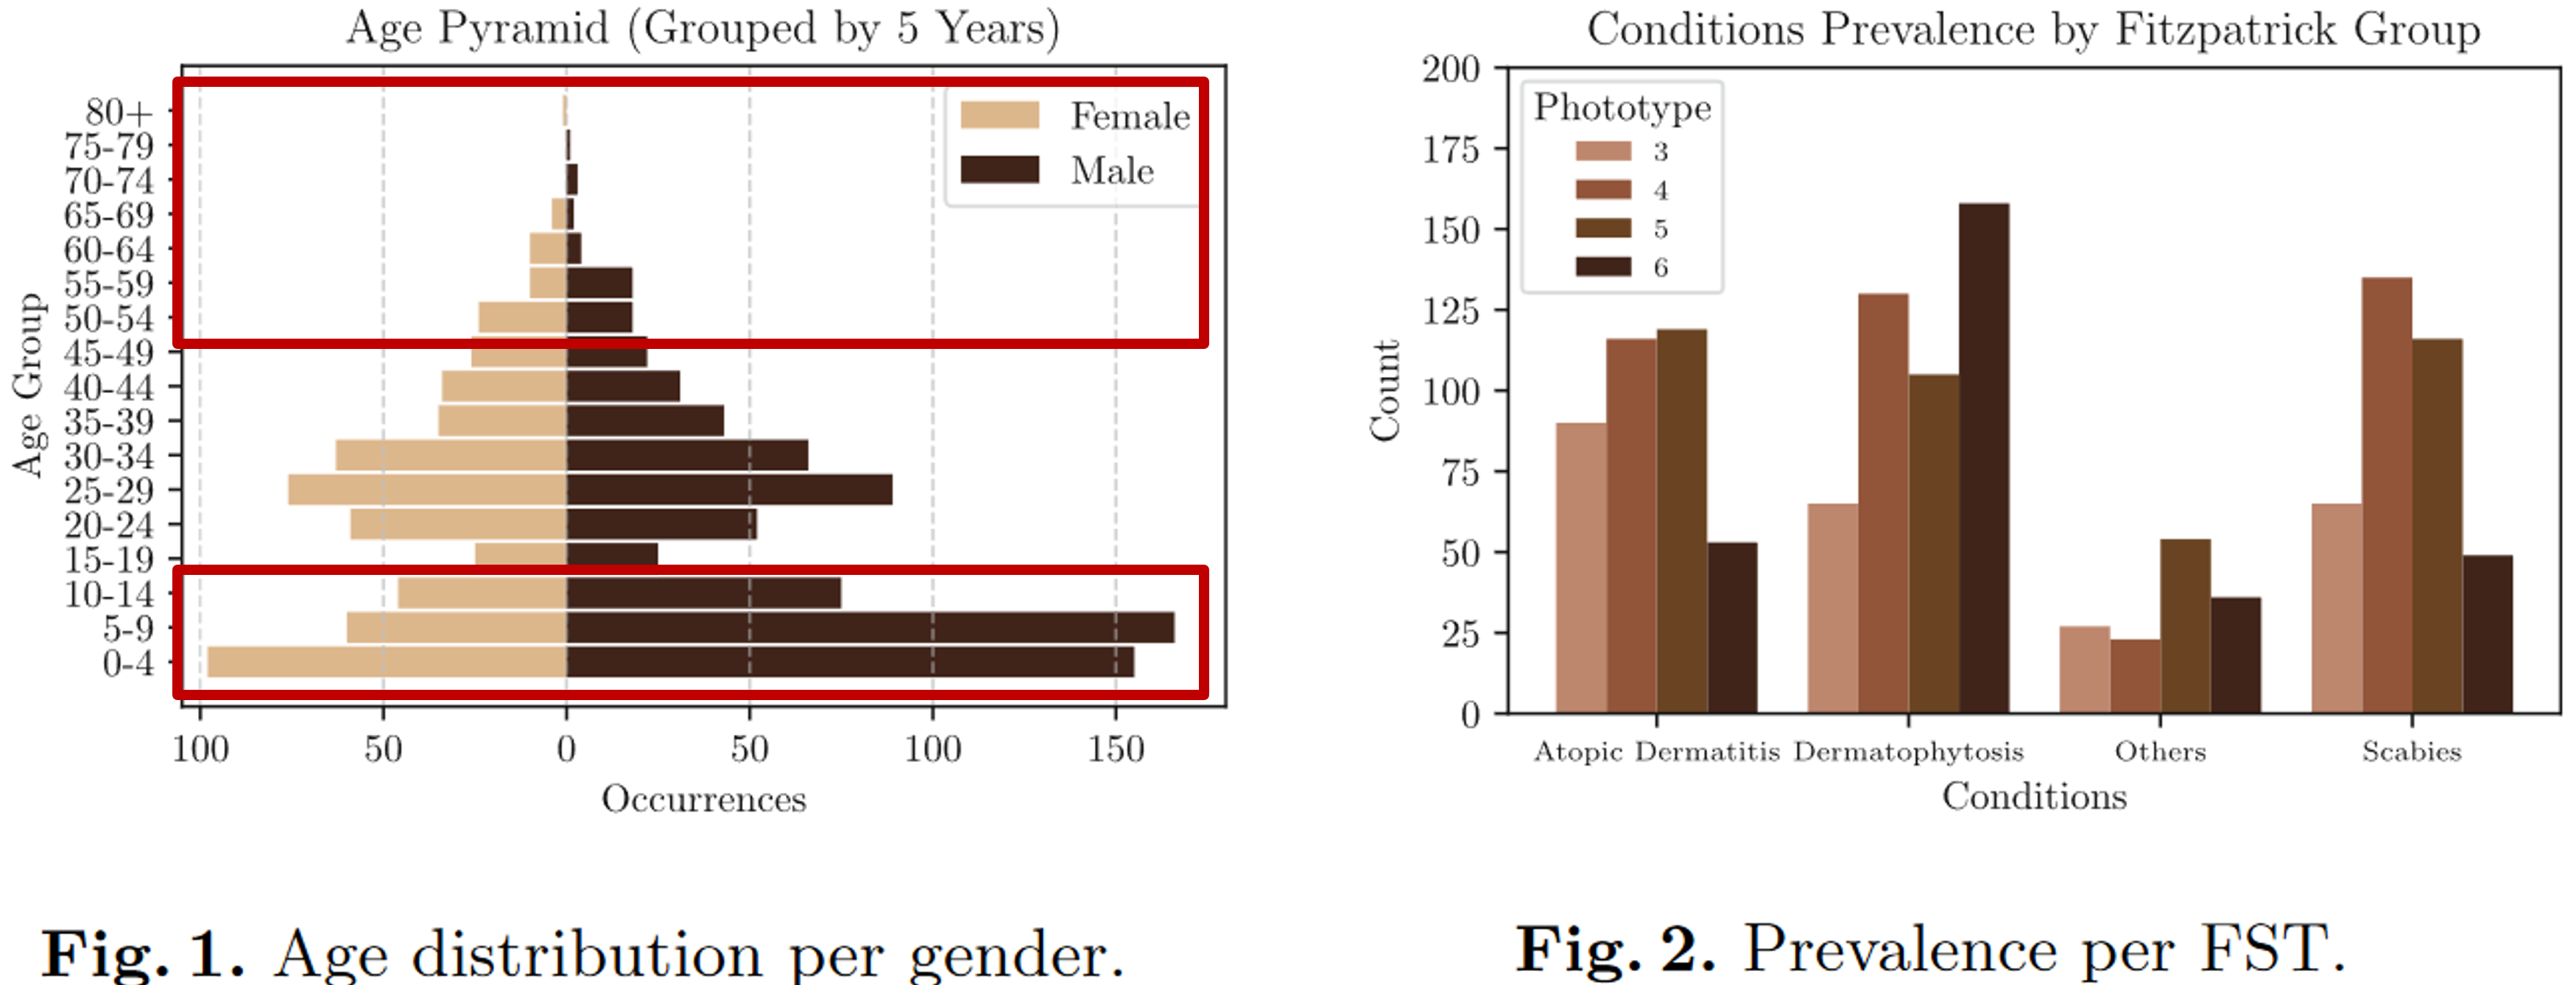
\includegraphics[width=0.9\textwidth]{figures/PASSIONDatasetDistributionPotentialImbalances.png}
			\caption{PASSION dataset distributions by \textcite{Gottfrois2024} - highlighting potential imbalances}
			\label{fig:PASSIONDistrImbalances}
		\end{figure}
		
		Even though this analysis does not take into consideration multiple images per case, these findings highlight representation disparities across several demographic and clinical factors. Such disparities should be considered during training and when evaluating fairness, especially when assessing subgroup-specific performance.
		
		It is important to note that the analysis provided only is a high-level overview at the group level. Detailed subgroup representation has not yet been assessed in detail. Due to the time limits of this thesis, this was deferred in favor of executing the stratified split experiment.
		
		To enable subgroup-level representation analysis, group-level dataset representation script should be extended accordingly. As the script output will increase substantially, manual comparison may become impractical. Therefore, automating the comparison and generating summaries of the largest disparities is recommended.
		
		
		\section{Reproducing PASSION Results}
		The overall model performance was consistent with the results reported in the PASSION paper.
		
		However, the group-level performance results could not be reproduced. Multiple inference runs with the same model and dataset produced inconsistent results. Introducing metadata linkage via filenames resolved this issue and provided stable, reproducible results. This confirms a reliable association between predictions and metadata, which is critical for fairness analysis.
		
		Currently, the checkpoint handling supports only evaluation. Additional adjustments are needed to fully support resumed training, particularly to ensure correct and reproducible handling of epochs and cross-validation folds.
		
		Those changes will be contributed to the PASSION code base to make the reproduction easier for others.
		
		While these extensive code improvements reduced the time available for fairness analysis, they are a critical enhancement to the robustness and usability of the PASSION evaluation.
		
		\section{PASSION Baseline Fairness Assessment} \label{sec:evaluation}
		
		The baseline fairness performance of \texttt{ResNet50} and \texttt{ResNet18} was assessed. This evaluation serves as a reproducible reference against which the impact of fairness mitigation strategies can be compared.
		\todo{consider instead:}
		The baseline fairness performance of \texttt{ResNet50} and \texttt{ResNet18} was evaluated to establish a reproducible reference point for assessing the effectiveness of subsequent fairness mitigation strategies.
		
		Only minor performance differences were observed between the two model variants (\autoref{tab:BaselineComparisonPerformance}), and the subgroup-level fairness patterns remained largely consistent (\autoref{tab:BaselineFairnessAssessment}). As a result, ResNet18 was considered a suitable substitution model for the experiments conducted in this thesis.
		
		Detailed findings are presented in the following subsections.
		
		\begin{table}[H]
			\centering
			\begin{tabularx}{\textwidth}{l *{2}{>{\centering\arraybackslash}X}}
				\toprule
				\textbf{Metric} & \textbf{ResNet18} & \textbf{ResNet50} \\
				\midrule
				\textbf{Overall} & & \\
				Accuracy & 0.69 & 0.71 \\
				Macro F1 & 0.69 & 0.71 \\
				Weighted F1 & 0.69 & 0.71 \\
				Balanced Accuracy & 0.69 & 0.71 \\
				
				\midrule
				\textbf{Class-Level F1 Scores} & & \\
				Eczema & 0.60 & 0.65 \\
				Fungal & 0.69 & 0.72 \\
				Others & 0.73 & 0.72 \\
				Scabies & 0.73 & 0.74 \\
				\bottomrule
			\end{tabularx}
			\caption{Baseline model performance comparison: ResNet18 vs. ResNet50.}
			\label{tab:BaselineComparisonPerformance}
		\end{table}
		
		\begin{table}[H]
			\centering
			\begin{tabularx}{\textwidth}{ >{\raggedright\arraybackslash}p{5.5cm}
					>{\centering\arraybackslash}X 
					>{\centering\arraybackslash}X 
					>{\centering\arraybackslash}X 
					>{\centering\arraybackslash}X}
				\toprule
				\textbf{Metric - Subgroup Mean} & \textbf{ResNet18} & \textbf{ResNet50} &  & \\
				\multicolumn{5}{l}{\textbf{Compared To Overall}}\\
				\midrule
				\multicolumn{5}{l}{\textbf{Overall}} \\
				avg & 0.49 & 0.49 & & \\
				best & 0.03 & 0.02 &  & \\
				worst & 0.73 & 0.74 &  &  \\
				median & 0.54 & 0.57 &  &  \\
				std. dev. sub pop. & 0.24 & 0.23 &  & \\
				std. dev. whole pop. & 0.23 & 0.22 &  &  \\
				\midrule
				\multicolumn{3}{l}{\textbf{Avg. Per Subgroup}} & \textbf{\# Subgroups} & \textbf{Min Support} \\
				fitzpatrick & 0.10 & 0.12 & 4 & 87 \\
				sex & 0.03 & 0.02 & 2 & 425 \\
				ageGroup & 0.46 & 0.48 & 14 & 2 \\
				country & 0.34 & 0.37 & 4 & 19 \\
				fitzpatrick, sex & 0.18 & 0.17 & 8 & 32 \\
				fitzpatrick, ageGroup & 0.67 & 0.63 & 47 & 1 \\
				fitzpatrick, country & 0.51 & 0.55 & 11 & 2 \\
				sex, ageGroup & 0.56 & 0.60 & 26 & 2 \\
				sex, country & 0.38 & 0.42 & 8 & 4 \\
				ageGroup, country & 0.73 & 0.60 & 30 & 1 \\
				fitzpatrick, sex, ageGroup & 0.70 & 0.74 & 81 & 1 \\
				fitzpatrick, sex, country & 0.54 & 0.57 & 19 & 1 \\
				fitzpatrick, ageGroup, country & 0.73 & 0.67 & 62 & 1 \\
				sex, ageGroup, country & 0.73 & 0.74 & 55 & 1 \\
				fitzpatrick, sex, ageGroup, country & 0.73 & 0.74 & 102 & 1 \\
				\bottomrule
			\end{tabularx}
			\caption{Baseline fairness assessment comparison: ResNet18 vs. ResNet50.}
			\label{tab:BaselineFairnessAssessment}
		\end{table}
		
		\subsection{Bias in the Baseline}
		\todo{link output}
		Subgroup fairness results revealed slight disparities but the trends are consistent. The summary of \autoref{tab:BaselineFairnessAssessment} highlights the following insights into existing biases:
		\begin{itemize}
			\item \textbf{Sex:} Only slight disparities indicated.
			\item \textbf{\gls{FST}:} Indications of existing biases, accompanied by an uneven support distribution.
   			\item \textbf{Age Group:} This attribute holds the largest disparities among the main categories. Some age groups had very low support (down to 0, the lowest existing group had 2).
			\item \textbf{Country:} Shows fairness disparities and skewed representation.
	    	\item \textbf{Intersectional Analysis:} Bias increase across more granular subgroup combinations. Even for attributes with lower individual disparities (e.g., \gls{FST}, sex), their combinations uncovered additional bias patterns. With more intersected dimensions, the disparities increased significantly.
		\end{itemize}
		
		To gain deeper insights, the data was evaluated on subgroup level in an exploratory analysis:
		\begin{itemize}
			\item \textbf{Sex:} Both models showed a slight bias toward women, with higher \gls{TPR} for female patients.
			\item \textbf{\gls{FST}:} Both models consistently privileged \gls{FST} V and underprivileged \gls{FST} VI. Notably, \gls{FST} III and VI showed different behavior across models, being more privileged in the big model.
			\item \textbf{Age:} The impact of age was relatively small on the \gls{FPR} but showed large disparities in the \gls{TPR} in both models. The age groups 0–14 and 25–29 were generally better off, whereas groups 20–24 and 30–69 were more often underprivileged. No samples for the 70+ group were available in the test data.
			\item \textbf{Intersectional Analysis:} Subgroup-level analysis revealed distinct patterns, such as males aged 15–59 being consistently underprivileged across both models. Also, subgroups tend to have very low support, which makes the fairness analysis less stable.
			\item \textbf{Country:} In both models, substantial differences emerged between countries. For example, Guinea performed better under the small model, while Malawi showed better results with the larger model. Tanzania remained underprivileged across both architectures.
		\end{itemize}
		
		Intersectional fairness issues also became apparent when combining protected attributes. For example, in the large model:
		\begin{itemize}
			\item \textbf{\gls{FST} VI in Madagascar and Tanzania} performed particularly poorly.
			\item \textbf{Guinea with \gls{FST} VI} still showed favorable outcomes, albeit slightly worse in ResNet50 compared to ResNet18. This indicates that the country might impact the model's bias stronger than the skin type.
		\end{itemize}
		
		Overall, the clearest fairness disparities were observed in subgroups related to the attributes \gls{FST}, sex, and country. Given PASSION’s goal to mitigate bias against highly pigmented skin tones, fairness issues with \gls{FST} VI are especially concerning. That some subgroups including \gls{FST} VI and specific countries perform well indicates, that the bias could stem from other origins, such as the image quality or the process on how the data was gathered in those countries. While this analysis provides a first systematic fairness evaluation, deeper investigations are necessary, particularly into age-related intersectional effects. The scripts provided enable further detailed analysis and subgroup comparisons.
		
		
		
		These findings reinforce the importance of evaluating fairness not only at group level but also across subgroups, as emphasized by \textcite{M79_Kearns_2018, M80_Kearns_2019}. As discussed in \autoref{chap:limitationslowSupport}, fairness metric volatility tends to increase when subgroup sample sizes are low. Collecting more data is thus essential to ensure robust assessments.
		 
		In the mean time, one potential mitigation strategy involves consolidating age groups, e.g., using an aggregation often used in dermatology. As neighboring age ranges often show similar behavior, merging them may help improve subgroup support without significantly hiding underlying fairness trends. This consolidation would also facilitate clearer fairness evaluations by reducing metric noise from very small subgroups.
		
		For further work, additional data collection efforts should prioritize Tanzania since the country is underrepresented which is consistently reflected in the model performance. Data quality or scarcity might be contributing to inconsistent results for this subgroup. Due to the sensitive medical nature of the images and personal limitations in handling such content, the images were not directly reviewed to support this hypothesis. It is, however, strongly recommended that the PASSION team conducts a thorough analysis of these cases.
		
		% \todo{Add link or reference to analysis scripts and generated data, possibly in appendix}
		
		\subsection{Subgroup-Level Insights}
		Using the aggregation of class-level equalized odds metrics, the assessment revealed substantial variance across subgroups. Privileged and underprivileged subgroups are consistently identifiable.
		
		While some groups showed stable behavior across classes, others shifted category depending on the evaluated class, which underlines the importance of per-class fairness computation in multiclass settings.	
		
		
		\subsection{Pipeline Challenges}
		
		Several technical limitations impacted the reliability and completeness of the fairness assessment:
		\begin{itemize}
			\item \gls{Fairlearn}’s default multiclass handling is limited. To overcome this, a custom implementation was required, which introduces complexity and potential inconsistencies with the intended methodology of researchers.
			\item In the report part where subgroups are classified regarding privilege level, some subgroups were suppressed. This affects fairness analysis negatively. The comparison to the \gls{Fairlearn} output revealed this issue. This proves that it is preferable to use well-established, tested libraries whenever possible.
			\item Manual aggregation of subgroup-level to model-level metrics as well as the cross-model comparison is currently not automated, reducing reproducibility and increasing error risk.
			\item For model comparisons, the approach of \textcite{Valentim_2019} of creating fairness comparison rations could be used for the automated reporting.
		\end{itemize}
		
		Despite these challenges, the evaluation successfully identified disparities among subgroup, supporting the idea that fairness analysis among subgroups is important for reducing biases in dermatology models, including PASSION.
		
		\subsection{Aggregation Trade-offs}
		Although aggregating fairness metrics at subgroup and model levels provides helpful summaries, it hide subgroup-specific effects. This must be considered when interpreting aggregated metrics.
		
		The proposed aggregation strategy was implemented due to the absence of ready-to-use multiclass equalized odds metrics in \gls{Fairlearn} or similar libraries. This illustrates the need for researchers to work together and implement suggested methodology improvements in the state-of-the art libraries.
		
		\section{Stratified Split Experiment}
		
		The evaluation of this experiment confirms that stratification strategies can influence fairness. The current findings suggest that including the attributes \textit{country} and \textit{fitzpatrick} in the stratification process can improve the fairness of models trained on the PASSION dataset. However, this improvement may negatively impact the overall model performance.
		
		These results should be interpreted with caution, given that the experiment faced several limitations. To achieve more statistically robust findings, additional data is required. Further experiments should be conducted using the available codebase. Based on the results, the current PASSION split could likely be refined. Moreover, analyzing subgroup-specific performance could inform future data collection efforts to achieve fairer outcomes.
		
		
		\subsection{Demographic Representation Across Subsets}
		Distribution analysis of the original PASSION split shows that the distributions between the subsets are balanced for some attributes (e.g., country, conditions\_PASSION), while others show notable discrepancies (fitzpatrick and sex). This suggests that the original split may have used country and conditions\_PASSION for stratification, possibly including impetig and ageGroup.
		\todo{link to appendix or github} 	%C:\Users\nadja\OneDrive\HSLU_Nadja\BAA\baa_on_git\results\reproducing_PASSION_results\analyzing_dataset_split	
		
		Interestingly, the dataset shows male overrepresentation, especially in the training set, despite slight female bias in model performance (see \autoref{tab:PASSIONSexDistribution}). Similarly, \gls{FST} IV and V are overrepresented in training data (\autoref{tab:PASSIONFstDistribution}), which may contribute to the observed bias. However, \gls{FST} VI is evenly distributed across the subsets, yet model performance remains poor. This suggests that data imbalance is not necessarily the sole cause of observed biases. Nevertheless, a more detailed subgroup-level analysis across all subsets is still essential for a robust interpretation.
		
		\begin{table}[H]
			\centering
			\begin{tabularx}{\textwidth}{l *{3}{>{\centering\arraybackslash}X}}
				\toprule
				\textbf{Set} & \textbf{Female} & \textbf{Male} & \textbf{Total} \\
				\midrule
				Training set & 539 (40.74\%) & 784 (59.26\%) & 1323 \\
				Test set & 152 (46.06\%) & 178 (53.94\%) & 330 \\
				Overall & 691 (41.8\%) & 962 (58.2\%) & 1653 \\
				\bottomrule
			\end{tabularx}
			\caption{PASSION Dataset: Sex distribution (train, test, overall).}
			\label{tab:PASSIONSexDistribution}
		\end{table}
				
		\begin{table}[H]
			\centering
			\begin{tabularx}{\textwidth}{l *{6}{>{\centering\arraybackslash}X} >{\centering\arraybackslash}X}
				\toprule
				\textbf{Set} & \textbf{I} & \textbf{II} & \textbf{III} & \textbf{IV} & \textbf{V} & \textbf{VI} & \textbf{Total} \\
				\midrule
				Training set & 1 (0.08\%) & -- & 275 (20.79\%) & 396 (29.93\%) & 344 (26.00\%) & 307 (23.20\%) & 1323 \\
				Test set & -- & -- & 79 (23.94\%) & 90 (27.27\%) & 84 (25.45\%) & 77 (23.33\%) & 330 \\
				Overall & 1 (0.06\%) & -- & 354 (21.42\%) & 486 (29.40\%) & 428 (25.89\%) & 384 (23.23\%) & 1653 \\
				\bottomrule
			\end{tabularx}
			\caption{PASSION Dataset: \glslink{FST}{FST} distribution (train, test, overall).}
			\label{tab:PASSIONFstDistribution}
		\end{table}	
		
		\subsection{Initial Training}
		As shown in \autoref{tab:StratifiedSplitstratified-seed42}, the fairness assessment of the initial model training indicated that, for strategy A (placing single records in training data), configuration 4 (using country and fitzpatrick) resulted in the fairest model overall, due to the analysis of reported \gls{EOD}:
		\begin{itemize}
			\item Lowest average and median
			\item Fairly low standard deviation
			\item Moderate worst-case fairness
		\end{itemize}
		
		
		For strategy B (\autoref{tab:StratifiedSplitstratified-seed32}), where singletons were put in the validation data, the fairest model was achieved by stratifying only on the target labels, due to the following:
		\begin{itemize}
			\item Low average and median
			\item Lowest standard deviation
			\item Moderate worst-case fairness
		\end{itemize}
		
		\begin{table}[H]
			\centering
			\scriptsize
			\begin{tabularx}{\textwidth}{l *{6}{>{\centering\arraybackslash}X}}
				\toprule
				\textbf{Metric} & \textbf{Split 1} & \textbf{Split 2} & \textbf{Split 3} & \textbf{Split 4} & \textbf{Split 5} & \textbf{Split 6} \\
				\midrule
				avg & 0.53 & 0.55 & \textcolor{red}{0.56} & \textcolor{teal}{0.48} & 0.54 & 0.55 \\
				best & 0.03 & 0.03 & 0.04 & 0.05 & \textcolor{teal}{0.01} & \textcolor{red}{0.08} \\
				worst & \textcolor{teal}{0.74} & 0.81 & \textcolor{red}{0.83} & 0.79 & 0.79 & 0.78 \\
				median & 0.55 & 0.54 & \textcolor{red}{0.60} & \textcolor{teal}{0.44} & 0.53 & 0.56 \\
				std. dev. sub pop. & 0.22 & 0.23 & \textcolor{red}{0.25} & 0.23 & 0.25 & \textcolor{teal}{0.22} \\
				std. dev. whole pop. & 0.21 & 0.22 & \textcolor{red}{0.24} & 0.23 & 0.24 & \textcolor{teal}{0.21} \\
				\bottomrule
			\end{tabularx}
			\caption{Stratified Split: Fairness summary (seed 42, single-record training stratification).}
			\label{tab:StratifiedSplitstratified-seed42}
		\end{table}
		
		\begin{table}[H]
			\centering
			\scriptsize
			\begin{tabularx}{\textwidth}{l *{6}{>{\centering\arraybackslash}X}}
				\toprule
				\textbf{Metric} & \textbf{Split 1} & \textbf{Split 2} & \textbf{Split 3} & \textbf{Split 4} & \textbf{Split 5} & \textbf{Split 6} \\
				\midrule
				avg & 0.51 & 0.55 & \textcolor{red}{0.57} & 0.55 & 0.55 & \textcolor{teal}{0.49} \\
				best & \textcolor{teal}{0.02} & 0.04 & 0.03 & 0.03 & \textcolor{red}{0.05} & 0.03 \\
				worst & 0.74 & 0.82 & \textcolor{red}{0.84} & 0.75 & \textcolor{teal}{0.71} & 0.73 \\
				median & 0.53 & 0.58 & 0.56 & 0.56 & \textcolor{red}{0.65} & \textcolor{teal}{0.50} \\
				std. dev. sub pop. & \textcolor{teal}{0.18} & \textcolor{red}{0.25} & 0.23 & 0.20 & 0.19 & 0.22 \\
				std. dev. whole pop. & \textcolor{teal}{0.17} & \textcolor{red}{0.25} & 0.22 & 0.20 & 0.18 & 0.21 \\
				\bottomrule
			\end{tabularx}
			\caption{Stratified Split: Fairness summary (seed 32, single-record validation stratification).}
			\label{tab:StratifiedSplitstratified-seed32}
		\end{table}
		
		Random splits also performed surprisingly well. Using strategy B, the highest level fairness was achieved in terms of the average and median, although there was higher variance. Using strategy A, the lowest standard deviation was achieved, though the fairness was lower overall.
		
		Based on these observations, and their performance overall, splits 1, 4, and 6 were selected for 5-fold cross-validation.
		
		\subsection{Cross-Validation}
		
		The results of the 5-fold cross-validation step confirmed that the fairest models for both single-record handling strategies were consistently produced by including \textit{country} and \textit{fitzpatrick} in the stratification (see \autoref{tab:StratifiedSplitstratified-seed32-crossVal}, \autoref{tab:StratifiedSplitstratified-seed42-crossVal}).
		
		\begin{table}[H]
			\centering
			\begin{tabularx}{\textwidth}{l *{3}{>{\centering\arraybackslash}X}}
				\toprule
				\textbf{Metric} & \textbf{Split 1} & \textbf{Split 4} & \textbf{Split 6} \\
				\midrule
				avg & \textcolor{red}{0.54} & 0.50 & \textcolor{teal}{0.48} \\
				best & \textcolor{teal}{0.03} & \textcolor{teal}{0.03} & \textcolor{teal}{0.03} \\
				worst & \textcolor{red}{0.75} & \textcolor{teal}{0.65} & 0.71 \\
				median & \textcolor{red}{0.57} & 0.55 & \textcolor{teal}{0.53} \\
				std. dev. sub pop. & \textcolor{red}{0.20} & \textcolor{teal}{0.16} & \textcolor{red}{0.20} \\
				std. dev. whole pop. & 0.19 & \textcolor{teal}{0.16} & \textcolor{red}{0.20} \\
				\bottomrule
			\end{tabularx}
			\caption{Stratified Split: Fairness summary (5-fold CV, seed 32, validation stratification).}
			\label{tab:StratifiedSplitstratified-seed32-crossVal}
		\end{table}
		
		\begin{table}[H]
			\centering
			\begin{tabularx}{\textwidth}{l *{3}{>{\centering\arraybackslash}X}}
				\toprule
				\textbf{Metric} & \textbf{Split 1} & \textbf{Split 4} & \textbf{Split 6} \\
				\midrule
				avg & \textcolor{red}{0.55} & \textcolor{teal}{0.50} & \textcolor{red}{0.55} \\
				best & \textcolor{teal}{0.04} & \textcolor{teal}{0.04} & \textcolor{red}{0.06} \\
				worst & \textcolor{red}{0.82} & \textcolor{teal}{0.77} & \textcolor{teal}{0.77} \\
				median & 0.54 & \textcolor{teal}{0.51} & \textcolor{red}{0.58} \\
				std. dev. sub pop. & \textcolor{red}{0.25} & 0.23 & \textcolor{teal}{0.22} \\
				std. dev. whole pop. & \textcolor{red}{0.24} & \textcolor{teal}{0.22} & \textcolor{red}{0.22} \\
				\bottomrule
			\end{tabularx}
			
			\caption{Stratified Split: Fairness summary (5-fold CV, seed 42, training stratification).}
			\label{tab:StratifiedSplitstratified-seed42-crossVal}
		\end{table}
		
		
		\subsection{Baseline Comparison}
		The final evaluation on the original test set (\autoref{tab:StratifiedSplitBaselineComparison}) confirms that applying stratified splitting impacts model fairness, especially at subgroup levels.
		Stratifying on \textit{country} and \textit{fitzpatrick} improved fairness, especially when single records were put in the training set. For the other strategy, results are mixed, but there is still a notable impact. Notably, the results are not directly comparable though due to the usage of different seeds in the split creation.
		
		\begin{table}[H]
			\centering
			\begin{tabularx}{\textwidth}{l *{3}{>{\centering\arraybackslash}X}}
				\toprule
				\textbf{Metric} & \textbf{Baseline} & \textbf{Strategy A} & \textbf{Strategy B} \\
				\midrule
				\multicolumn{4}{l}{\textbf{Overall}} \\
				avg & 0.49 & \textcolor{teal}{0.47} & \textcolor{red}{0.51} \\
				best & 0.03 & \textcolor{teal}{0.02} & \textcolor{black}{0.03} \\
				worst & 0.73 & \textcolor{red}{0.75} & \textcolor{red}{0.74} \\
				median & 0.54 & \textcolor{teal}{0.51} & \textcolor{black}{0.54} \\
				std. dev. sub pop. & 0.24 & \textcolor{teal}{0.21} & \textcolor{teal}{0.22} \\
				std. dev. whole pop. & 0.23 & \textcolor{teal}{0.21} & \textcolor{teal}{0.22} \\
				
				\midrule
				\multicolumn{4}{l}{\textbf{Avg. Per Subgroup}} \\
				fitzpatrick & 0.10 & \textcolor{red}{0.14} & \textcolor{red}{0.19} \\
				sex & 0.03 & \textcolor{teal}{0.02} & \textcolor{black}{0.03} \\
				ageGroup & 0.46 & \textcolor{teal}{0.43} & \textcolor{red}{0.54} \\
				country & 0.34 & \textcolor{red}{0.36} & \textcolor{teal}{0.33} \\
				fitzpatrick, sex & 0.18 & \textcolor{red}{0.20} & \textcolor{red}{0.28} \\
				fitzpatrick, ageGroup & 0.67 & \textcolor{teal}{0.60} & \textcolor{red}{0.68} \\
				fitzpatrick, country & 0.51 & \textcolor{black}{0.51} & \textcolor{teal}{0.50} \\
				sex, ageGroup & 0.56 & \textcolor{teal}{0.53} & \textcolor{red}{0.62} \\
				sex, country & 0.38 & \textcolor{red}{0.41} & \textcolor{teal}{0.37} \\
				ageGroup, country & 0.73 & \textcolor{teal}{0.48} & \textcolor{teal}{0.64} \\
				fitzpatrick, sex, ageGroup & 0.70 & \textcolor{red}{0.75} & \textcolor{red}{0.74} \\
				fitzpatrick, sex, country & 0.54 & \textcolor{teal}{0.51} & \textcolor{black}{0.54} \\
				fitzpatrick, ageGroup, country & 0.73 & \textcolor{teal}{0.60} & \textcolor{teal}{0.70} \\
				sex, ageGroup, country & 0.73 & \textcolor{teal}{0.69} & \textcolor{red}{0.74} \\
				fitzpatrick, sex, ageGroup, country & 0.73 & \textcolor{red}{0.75} & \textcolor{red}{0.74} \\
				\bottomrule
			\end{tabularx}
			\caption{Stratified Split: Fairness comparison: baseline vs. stratified variants.}
			\label{tab:StratifiedSplitBaselineComparison}
		\end{table} 
		
		Although the stratified variants showed improved fairness, there was a noticeable drop in overall model performance (see \autoref{tab:StratifiedSplitBaselineComparisonPerformance}). This was somewhat expected, given that the baseline used the full original training set, whereas the stratified variants employed an additional train-validation split, which reduces the number of training samples. Both the F1-score and balanced accuracy decreased compared to the baseline. Strategy~B in particular exhibited the poorest performance across most metrics, likely due to its small training set which lacks certain rare cases.
		
		This illustrates the trade-off between fairness and predictive performance that must be carefully managed in real-world applications.
		
		\begin{table}[H]
			\centering
			\begin{tabularx}{\textwidth}{l *{3}{>{\centering\arraybackslash}X}}
				\toprule
				\textbf{Metric} & \textbf{Baseline} & \textbf{Strategy A} & \textbf{Strategy B} \\
				\midrule
				Accuracy             & 0.69 & \textcolor{red}{0.61} & \textcolor{red}{0.59} \\
				Macro F1             & 0.69 & \textcolor{red}{0.61} & \textcolor{red}{0.59} \\
				Weighted F1          & 0.69 & \textcolor{red}{0.62} & \textcolor{red}{0.59} \\
				Balanced Accuracy    & 0.69 & \textcolor{red}{0.62} & \textcolor{red}{0.60} \\
				\bottomrule
			\end{tabularx}
			
			\caption{Stratified Split: Performance comparison: baseline vs. stratified variants.}
			\label{tab:StratifiedSplitBaselineComparisonPerformance}
		\end{table}
		
		\section{Code Contribution}
		The code written during this thesis will be provided as a pull request to the PASSION GitHub project, so that the team can use it for their future work.
		
	\chapter{Outlook}
		This chapter summarizes the concrete recommendations to overcome the limitations of the current work. This includes e.g., revising the metadata used in PASSION, and extending the analytical tools used.
		
		It also provides ideas, such as adding more diverse data and combining PASSION with other dermatology datasets to improve bias detection and aim for a more complete dataset. Also, it is emphasized to check the \autoref{app:listOfBiases} to get an overview over existing biases and their relevance for PASSION.
		
		These measures aim to enhance the practical applicability of the results and support the development of fair, generalizable \gls{ML} models in dermatology.
	
		
		\section{PASSION Dataset Improvements}
		To improve the fairness assessment capabilities of the PASSION dataset, the following dataset improvements are proposed:
		\begin{itemize}
			\item Include the missing metadata attributes identified in \autoref{chap:datasetAssessmentMetadataEvaluation} (e.g., socioeconomic status, clinic type, image quality) to enable a more comprehensive fairness evaluation. Ensure to assess the ethical implications before collecting such data.
			\begin{itemize}
				\item Investigate whether \textit{ethnicity} and \textit{disabilities} influence the presentation or prevalence of dermatological conditions before adding them to the dataset.
			\end{itemize}
						
			\item Clarify the intended purpose of the \textit{country} attribute and replace or supplement it with more precise alternatives, as discussed in \autoref{chap:datasetAssessmentMetadataEvaluation}.
			
			\item Refine the "other" condition category by breaking it down into more specific labels to improve diagnostic granularity and fairness assessment per condition.
			
			\item Incorporate healthy skin samples into the dataset to allow for a more balanced classification task and to mitigate potential bias.
			
			\item Explore whether combining PASSION with other dermatology datasets enhances generalization across the full \gls{FST} range.
		\end{itemize}
		
		
		\section{Training Process Improvements}
		To enable full reproducibility and extensibility, further work should include:
		
		\begin{itemize}
			\item Finalizing checkpoint loading support for resumed training by correctly tracking and reloading epochs and folds.
			\item Incorporating automated tests to verify linkage integrity and model reproducibility.
		\end{itemize}
		
		
		\section{Fairness Assessment Process Improvements}
		The measures to improve the fairness assessment process further are:
		\begin{itemize}
			\item Extend the existing dataset representation script, as described in \autoref{chap:datasetAssessmentExecution}, to support subgroup-level analysis, automated comparison, and image-level analysis.
			\item Replace confusion-matrix-based fairness calculations with direct \texttt{MetricFrame}-based computation to streamline and unify the process.
			\item Improve subgroup handling in the fairness evaluation pipeline to include low-support groups more reliably.
			\item Automate all metric aggregation steps and document all assumptions clearly to enhance reproducibility.
			\item Introduce the model comparison ratio used by \textcite{Valentim_2019}.
		\end{itemize}		
		
		\section{Fairness Assessment Results Review}
		The existing fairness assessment results can be extended with those actions:
		\begin{itemize}
			\item Perform the representation analysis of relevant subgroups, as described in \autoref{chap:datasetAssessmentMethod} using the extended script, to determine whether observed unfairness stems from distribution imbalances at subgroup level.	
			
			\item Evaluate model performance across \gls{FST} types V and VI more closely and take measures if bias exist. \todo{check if this will still be needed}
			
			\item Evaluate worst-case metrics and \gls{EOR} during the fairness assessment and model comparisons as suggested in \autoref{chap:ContextFairnessMetrics}. The metric computation is already included in the script but not yet useful due to missing data.
			
			\item Incorporate multiple training seeds for each experiment (also for the baseline) for drawing statistically valid conclusions about fairness across model variations and mitigation methods.
		\end{itemize}
		
		Implementing these measures will enhance the dataset’s ability to support fair, robust, and generalizable \gls{ML} models in dermatology.
	
	
	
	
		% Lists and References
		\newpage
	
	
	\chapter{\bibname}
		\printbibliography[heading=none]
		
		%\bibliographystyle{ieeetr}
		%\footnotesize\bibliography{references}
		
		
		%----------------------------------------------------------------------------------------
		%	APPENDIX
		%----------------------------------------------------------------------------------------
		\newpage
		\appendix
		\begin{appendices}
		
	
			\chapter{PASSION Data Analysis Scripts}\label{app:PASSIONdataAnalysisScripts}
			The PASSION team provides a \gls{JupyterNotebook} with code examples and analysis scripts. They are listed in \autoref{tab:PASSION_scripts} together with their relevance to this thesis. The most relevant scripts are those related to demographic distributions of the chosen attributes, since they help identifying potential data imbalances. Scripts that lay the foundation for further analysis are somewhat relevant, while all other scripts are irrelevant for this thesis.
			
			\begin{table}[H]
				\centering
				\begin{threeparttable}
					\begin{tabularx}{\textwidth}{>{\hsize=.25\hsize\raggedright}X>{\hsize=.41\hsize}X>{\hsize=.34\hsize}X}
						\toprule
						\textbf{Script Title}       & \textbf{Description} & \textbf{Relevance - Reasoning}       \\ \midrule
						Distribution of \glspl{FST} &
						Counts and visualizes the skin type distribution  &
						\textbf{High} - Insight into demographic distributions \\
						\hline
						Regrouping Malawi and Tanzania to EAS &
						Data aggregation due to dataset size and geographical proximity &
						\textbf{Medium} - Might impact interpretation of the results of the following scripts \\
						\hline
						Linking CSV Data with Image Files & 
						Mapping between data records and images. &
						\textbf{Medium} - Basis for other analyses \\
						\hline
						Extracting and Comparing Subject IDs &
						Dataset verification regarding completeness &
						\textbf{Low} - No insight in regards of demographic distribution \\
						\hline
						Conditions by Country &
						Correlation between clinical conditions and country &
						\textbf{Low} - The attribute \textit{country} is out of scope of this thesis \\
						\hline
						Body Localizations by Conditions &
						Correlation between the condition and primarily affected body parts &
						\textbf{Low} - No insight in regards of demographic distribution \\
						\hline
						Impetigo Cases &
						Total count of impetigo cases and proportion to all cases &
						\textbf{Low} - No insight in regards of demographic distribution\tnote{*} \\
						\bottomrule
					\end{tabularx}
					\begin{tablenotes}
						\footnotesize
						\item[*] Research is divided on which demographic factors influence the prevalence of impetigo \autocites{Romani_2017}{Aleid_2024}.
					\end{tablenotes}
				\end{threeparttable}
				
				\caption{PASSION dataset - existing analysis scripts \autocite{Gottfrois2024}}
				\label{tab:PASSION_scripts}
			\end{table}
			
		\chapter{List of Biases}\label{app:listOfBiases}
		\autoref{tab:biases_types_appendix} summarizes the categorization of bias types. The categories and corresponding biases are described below. Each bias is presented with a definition, an example, a possible mitigation strategy, and its relevance and recommendations for PASSION. Mitigation strategies and examples without citations are based on conclusions drawn from the bias descriptions and the reviewed literature. It is encouraged to further enhance this list.
		
		The italicized part in the following chapter titles indicates the relevance of each category or bias for PASSION (e.g., \textit{high}), based on the following criteria:
		\begin{itemize}
			\item \textbf{High.} Directly applicable to PASSION, both in terms of the \gls{teledermatology} setting and available metadata; likely to provide valuable insights or improvements. Also, crucial demographic biases are included as high, since PASSION's aim is to create more accessible \gls{AI} models.
			\item \textbf{Medium.} Generally relevant to diagnostic \gls{AI} and PASSION, but do not seem to have the biggest impact towards PASSION's primary goals.
			\item \textbf{Low.} Related to PASSION but only limited. E.g., in the far future it could potentially impact PASSION.
			\item \textbf{Not Applicable.} Not relevant for PASSION due to fundamental differences in domain, type of data, or type of model. For this categorization, no mitigation methods are listed.
		\end{itemize}
		
		Notably, at the time of writing this thesis, detailed information on the exact data selection process behind PASSION and the rationale for certain decisions was not available. The PASSION relevance sections therefore aim to highlight potential impacts based on the available documentation and observed characteristics of the dataset.
		
		\begin{table}[H]
			\centering
			\begin{threeparttable}
				\begin{tabularx}{\textwidth}{>{\tblWidthDescription}X|>{\tblWidthContext}X|>{\tblWidthContext}X}
					\toprule
					\textbf{Bias} & \multicolumn{2}{c}{\textbf{Mentioned in Context of}} \\
					& \textbf{\gls{ML}} & \textbf{Dermatology} \\
					%	\midrule
					\multicolumn{3}{l}{\bolditalic{Data Collection}} \\ 
					
					Sampling Biases & X\tnote{1,2,3} & X\tnote{4} \\
					Representation Biases & X\tnote{1} & X\tnote{5,6} \\
					Measurement Biases & X\tnote{1,3} & X\tnote{4,6} \\
					Research Biases & X\tnote{7} & X\tnote{4} \\
					Feature Representation Biases & X\tnote{1,3} & X\tnote{4} \\
					Imaging Biases & & X\tnote{5} \\
					Medical Biases & X\tnote{8} & X\tnote{4} \\
					Temporal Biases & X\tnote{1} & X\tnote{4}\\
					
					%	\midrule
					\multicolumn{3}{l}{\bolditalic{Algorithmic Design}} \\ 
					Algorithmic Biases & X\tnote{1} & \\
					External Influence Biases & X\tnote{1} & X\tnote{4} \\
					
					%	\midrule
					\multicolumn{3}{l}{\bolditalic{User Interactions}} \\
					Cognitive Biases & X\tnote{1,7} & X\tnote{4} \\
					Behavioral Biases & X\tnote{1,3} & X\tnote{4,5} \\
					Publication Biases &  & X\tnote{4} \\
					Medical Biases & X\tnote{} & X\tnote{4} \\
					
					\bottomrule
				\end{tabularx}
				\begin{tablenotes}
					\footnotesize
					\begin{minipage}{0.33\textwidth}\raggedright
						\item[1] \autocite{Mehrabi_2021}
						\item[2] \autocite{HP_2022}
						\item[3] \autocites{Mester_2022}
					\end{minipage}%
					\begin{minipage}{0.33\textwidth}\raggedright
						\item[4] \autocite{Chakraborty_2024}
						\item[5] \autocite{Young_2020}
						\item[6] \autocite{Montoya_2025}
					\end{minipage}%
					\begin{minipage}{0.33\textwidth}\raggedright
						\item[7] \autocites{Mester_2017}
						\item[8] \autocite{Delgado-Rodriguez_2004}
					\end{minipage}%
				\end{tablenotes}
			\end{threeparttable}
			\caption{Bias categories - grouped according the \glsentryshort{ML} lifecycle of \textcite{Mehrabi_2021}}
			\label{tab:biases_types_appendix}
		\end{table}
		
		
		\section{Category: Sampling Bias, \textit{high}} \label{app:biasCategorySamplingBiasHigh}
		Sampling biases occur when the process of collecting data results in samples that are not representative of the broader population. These biases affect the generalizability of \gls{ML} models, especially in medical applications, where population diversity is crucial. Non-random or selective sampling can lead to serious consequences in terms of fairness and effectiveness of \gls{AI} systems \autocite{Mehrabi_2021, HP_2022}.
		
		\subsection{Sampling Bias, \textit{high}}
		\begin{itemize}
			\item \textbf{Definition:} Bias introduced through non-random sampling of subgroups, leading to poor generalization \autocite{Mehrabi_2021}.
			\item \textbf{Example:} An \gls{ML} model trained predominantly on patients with low pigmented skin may underperform on images of patients with highly pigmented skin \autocite{Gottfrois2024}.
			\item \textbf{Mitigation Strategy:} Ensure a truly random and inclusive sampling strategy across diverse factors, e.g., by including lots of diverse sources.
			\item \textbf{PASSION Relevance:} PASSION already aims to address sampling bias against highly pigmented skin \autocite{Gottfrois2024}. However, if the included data is not truly representative across populations (e.g., over-representation of certain countries, sex, age, skin tone), it could still result in sampling bias.
			It should be noted that the less pigmented skin tones should also be included in the PASSION dataset to ensure the model generalize among all \glspl{FST}.
		\end{itemize}
		
		\subsection{Selection Bias, \textit{high}}
		\begin{itemize}
			\item \textbf{Definition:} This bias arises when only a specific subset of the population is used, which is not representative \autocites{Mester_2022, Mester_2017,Chakraborty_2024}.
			\item \textbf{Example:} Training a model only on adult data, when the target population includes children.
			\item \textbf{Mitigation Strategy:} Ensure that data exists for all possible values of metadata attributes and their combinations.
			\item \textbf{PASSION Relevance:} PASSION may be affected by selection bias regarding age, \gls{FST}, country, and even target labels, as not all possible values are represented. For example, the category "Others" in the condition labels suggests that additional, unlabeled categories exist beyond the three explicitly named. Also, there are more countries in Sub-Saharan Africa - however, the intention of the country attribute should be refined before trying to cover all countries, as the effort would probably be massive. If bias exists for the country, also assess whether it is the symptom of another bias source.
		\end{itemize}
		
		\subsection{Systematic Selection Bias, \textit{high}}
		\begin{itemize}
			\item \textbf{Definition:} A form of selection bias where chosen samples differ systematically from the general population \autocite{Chakraborty_2024, c5,c6,c33}.
			\item \textbf{Example:} Including only hospitalized patients in a dataset, while most cases are treated in without hospitalization. This especially occures in studies conducted in regional referral centers \autocite{Chakraborty_2024, c5,c6,c33}.
			\item \textbf{Mitigation Strategy:} Include mild, moderate, and severe cases from various clinical settings.
			\item \textbf{PASSION Relevance:} If PASSION uses data only from dermatology centers treating severe cases, it introduces systematic selection bias. In that case, other sources should be added.
			Other possible systematic biases should be checked.
		\end{itemize}
		
		\subsection{Ascertainment Bias, \textit{high}}
		\begin{itemize}
			\item \textbf{Definition:} A systematic distortion arising from the method by which participants or data are selected for inclusion \autocite{Chakraborty_2024, c5}.
			\item \textbf{Example:} Studies on STD prevalence conducted only in public clinics may overlook patients from higher-income backgrounds who go to private practitioners \autocite{Chakraborty_2024, c5}.
			\item \textbf{Mitigation Strategy:} Use allocation concealment and blinding to avoid this bias \autocite{Chakraborty_2024, c5}.
			Also, ensure that data is collected from a diverse range of sources, e.g., including both public and private healthcare facilities.
			\item \textbf{PASSION Relevance:} If PASSION’s dataset is composed mostly of patients from certain types of clinics, it may not generalize well to other socioeconomic groups. PASSION's metadata would need to enhanced with such information to find these kind of impairments. There could be further distortions, therefore, the selection process should be reviewed critically.
		\end{itemize}
		
		\subsection{Availability Bias, \textit{high}}
		\begin{itemize}
			\item \textbf{Definition:} Overreliance on easily accessible data rather than the most representative data \autocites{Chakraborty_2024, c9, c10}.
			\item \textbf{Example:} Using only online available datasets for skin conditions may underrepresent rare diseases.
			\item \textbf{Mitigation Strategy:} Actively seek underrepresented data sources, especially for less common or less documented skin types.
			\item \textbf{PASSION Relevance:} PASSION is taking efforts to tackle this bias in dermatology \glspl{AI} overall by gathering data on \gls{FST} III to VI. Within the project, PASSION may reflect availability bias by primarily sourcing data from clinics or sources that were most accessible during collection, potentially excluding patients in remote or underrepresented regions within Sub-Saharan Africa. If that is the case, it is crucial that PASSION finds a way to include those regions as well, as they are probably the most vulnerable.
		\end{itemize}
		
		\subsection{Survivorship Bias, \textit{medium}}
		\begin{itemize}
			\item \textbf{Definition:} Only using data from so-called survivors, i.e., subjects that make it through a certain threshold or are retained in the dataset, ignoring those who were lost earlier \autocite{Mester_2022, Silfwer_2017}.
			\item \textbf{Example:} The original example of the World War II airplanes connects the bias indeed to only looking at data of surviving subjects \autocite{Silfwer_2017}. However, as \textcite{Mester_2022} indicates, also data records which survived pre-selections in the data collection process can be survivors. E.g., evaluating the success of a treatment based only on patients who completed it, ignoring those who dropped out due to side effects could lead to survivorship bias.
			\item \textbf{Mitigation Strategy:} Account for dropout rates and include cases from a wide range of medical access points.
			\item \textbf{PASSION Relevance:} Patients who are unable to attend the clinics may be excluded from the current dataset, potentially introducing survivorship bias. A more severe implication arises if certain dermatological conditions are life-threatening or correlate with other lethal diseases—these cases may be underrepresented. Therefore, efforts should be made to ensure such conditions are included in the dataset where possible, especially the early stages to allow for an early triage.
		\end{itemize}
		
		
		\section{Category: Representation Biases}\label{app:biasCategoryRepresentationBiasesHigh}
		Representation biases occur when a sample used to train or evaluate a \gls{ML} model fails to adequately reflect the diversity of the target population. These biases can lead to underperformance for certain subgroups and may negatively impact the fairness and accuracy of a model \autocite{Mehrabi_2021}.
		
		\subsection{Representation Bias, \textit{high}}
		\begin{itemize}
			\item \textbf{Definition:} Representation bias arises based on how the sampling during the data collection project is conducted. Non-representative sampling leads to missing subgroups or other representation anomalies, leading to missing or misrepresented characteristics in the data. Popular \gls{ML} datasets suffer from this bias \autocite{Mehrabi_2021,M142_Shankar_2017}.
			\item \textbf{Example:} If a skin disease detection model is trained predominantly on \gls{FST} I-III, it may struggle to accurately diagnose conditions in individuals with darker skin tones (\gls{FST} IV-VI), as seen in available dermatology models \autocite{Gottfrois2024}.
			\item \textbf{Mitigation Strategy:} A potential mitigation strategy could involve ensuring a more balanced representation and periodical reassessment to ensure inclusion over time.
			\item \textbf{PASSION Relevance:} PASSION attempts to mitigate representation bias in existing dermatology \gls{AI} models by including more FST skin types, but challenges may still exist. The dataset could still lack full representation of all diverse skin conditions and demographic factors, leading to potential misdiagnoses or underperformance for specific subgroups.
			It is suggested to include rare and diverse skin conditions and other demographic factors.
		\end{itemize}
		
		\subsection{Population Bias, \textit{high}}
		\begin{itemize}
			\item \textbf{Definition:} Population bias occurs when the sample's demographic characteristics (such as age, sex, or ethnicity) do not align with the target population, leading to non-representative data \autocite{M120_Olteanu_2019, Mehrabi_2021}.
			\item \textbf{Example:} \textcite{M64_Hargittai_2007} mentioned multiple demographic biases related to this bias, e.g., ethnicity. If a dataset is predominantly comprised of one ethnic group, a dermatology model trained on this data may not generalize well to other ethnic groups, if e.g., the manifestation of skin diseases varies across ethnicities.
			\item \textbf{Mitigation Strategy:} A mitigation strategy could involve collecting data from diverse populations and ensuring the dataset reflects the target population’s demographic diversity, particularly for ethnicities and age groups that may exhibit different disease manifestations.
			\item \textbf{PASSION Relevance:} PASSION might be impacted by population bias if it is insufficiently diverse in terms of patient demographics (e.g., ethnicity, age). The dataset needs to ensure that skin diseases are accurately represented across different population groups to avoid skewing results and compromising diagnostic accuracy. In order to evaluate the ethnic diversity, corresponding metadata should be added to the model, if the manifestations of skin diseases indeed vary among ethnicity.
		\end{itemize}
		
		\subsection{Aggregation Bias, \textit{high}}
		\begin{itemize}
			\item \textbf{Definition:} Aggregation bias occurs when conclusions drawn from the entire population do not apply to individual subgroups, leading to incorrect or generalized assumptions. This bias arises when significant differences between subgroups (such as sex or ethnicity) are not properly accounted for \autocite{Mehrabi_2021,M144_Suresh_2021}.
			\item \textbf{Example:} A diagnostic model trained on a heterogeneous dataset might fail to capture how skin diseases manifest differently across sexes or ethnic groups or more dimensional subgroups, potentially leading to misdiagnosis or unequal treatment recommendations \autocite{M144_Suresh_2021, Mehrabi_2021}.
			\item \textbf{Mitigation Strategy:} To mitigate aggregation bias, the model should incorporate subgroup-specific data and analysis, ensuring that disease manifestations are correctly accounted for and tailored to different demographic characteristics \autocite{M144_Suresh_2021,Mehrabi_2021}. It is especially important to do the analysis based on the model results, as the bias can also occur when (sub-)groups are equally represented in the data \autocite{Mehrabi_2021}. 
			\item \textbf{PASSION Relevance:} Aggregation bias is a significant concern in PASSION, since it involves multiple sensitive demographic factors which impact skin disease prevalence and appearance. The model needs to account for these factors to avoid generalized conclusions that might harm certain subgroups.
		\end{itemize}
		
		\subsection{Simpson's Paradox, \textit{high}}
		\begin{itemize}
			\item \textbf{Definition:} Simpson's Paradox is a form of aggregation bias where trends that appear in aggregated data may reverse when the data is disaggregated into subgroups. This paradox can lead to misleading conclusions if not properly addressed \autocite{Mehrabi_2021}.
			\item \textbf{Example:} A dataset may show that skin disease detection is more accurate overall for a specific demographic group, but when the data is broken down by age or skin type, the trend reverses for certain subgroups.
			\item \textbf{Mitigation Strategy:} A mitigation strategy would involve analyzing data at both the aggregated and disaggregated levels, ensuring that subgroup-specific trends are considered to avoid false conclusions or the reversal of apparent associations.
			\item \textbf{PASSION Relevance:} Simpson’s Paradox could be an issue in PASSION if aggregated data from different subgroups results in misleading conclusions. For example, overall accuracy per \glspl{FST} and sexes may appear high, but specific skin conditions in certain \gls{FST}-sex-subgroups could have lower accuracy when analyzed separately.
		\end{itemize}
		
		
		\section{Category: Measurement Biases, \textit{medium}} \label{biasCategoryMeasurementBiasesMedium}
		Measurement biases occur when the process of choosing, using, or measuring features leads to inaccurate or misleading results. These biases can emerge from various sources such as mismeasured variables, subconscious expectations of researchers, or inconsistencies in human annotation, and they can significantly affect the reliability of the dataset \autocite{Mehrabi_2021, M144_Suresh_2021}.
		
		\subsection{Measurement Bias, \textit{high}}
		\begin{itemize}
			\item \textbf{Definition:} Measurement bias occurs when features or metadata attributes are inaccurately measured or selected (e.g., \glspl{proxyVar}), leading to incorrect interpretations of the outcome \autocite{Mehrabi_2021}.
			\item \textbf{Example:} A \gls{proxyVar} it could lead to misinterpretation of the data \autocite{Wang_2021}. For instance, the country of origin or \gls{FST} may not directly correlate with ethnic or genetic background, potentially skewing results if those factors impact skin conditions.
			\item \textbf{Mitigation Strategy:} To mitigate measurement bias, careful consideration should be given to the choice of attributes used in the dataset. Avoiding \gls{proxyVar} relevant factors could improve the accuracy of the data and its interpretation.
			\item \textbf{PASSION Relevance:} In the context of the PASSION dataset, measurement bias could arise if country of origin is misused as a \gls{proxyVar} for ethnicity. The country of origin is not directly related to genetic predispositions or skin conditions. This could result in misleading conclusions about skin diseases across different demographic groups, potentially amplifying health disparities.
			Instead focus on medically relevant attributes.
		\end{itemize}
		
		\subsection{Observer Bias, \textit{medium}}
		\begin{itemize}
			\item \textbf{Definition:} Observer bias occurs when researchers or testers influence the results by projecting their expectations or perceptions onto the data collection process, or when different observers report the same observation differently \autocite{Mester_2022, Chakraborty_2024, c29, c26}.
			\item \textbf{Example:} A researcher may subconsciously interpret certain skin disease symptoms differently based on their own expectations or biases, leading to inconsistent data collection or interpretation \autocite{Chakraborty_2024}.
			\item \textbf{Mitigation Strategy:} To address observer bias, standardized training for annotators and a clear, objective set of criteria for diagnosis could be implemented \autocite{Montoya_2025}. Additionally, using multiple annotators and cross-checking results can help reduce the impact of individual biases.
			\item \textbf{PASSION Relevance:} In PASSION, observer bias could affect the consistency and reliability of skin disease annotations. Different personal experiences could lead to inaccurate classifications, particularly for diseases that are subjective in appearance.
		\end{itemize}
		
		\subsection{Annotator Bias, \textit{high}}
		\begin{itemize}
			\item \textbf{Definition:} Annotator bias is a form of observer bias where human annotators are influenced by personal background, expectations, or external factors, which can lead to inconsistent or skewed labeling of data \autocite{Montoya_2025}.
			\item \textbf{Example:} According to \textcite{Montoya_2025}, several factors like the scale order or image context can change how an annotator labels the skin tone, due to personal or cultural biases.
			\item \textbf{Mitigation Strategy:} To reduce annotator bias, \textit{"greater transparency, standardized procedures, and careful consideration of annotator biases"} are needed \autocite{Montoya_2025}. Maybe, the use of automated tools for initial labeling could provide more objectivity in the process.
			\item \textbf{PASSION Relevance:} In PASSION, annotator bias could particularly affect the labeling of skin tones, which are somewhat dependent on individual perception. This bias could further lead to inconsistent classifications of skin conditions across different demographic groups.
		\end{itemize}
		
		\subsection{Recall Bias, \textit{low}}
		\begin{itemize}
			\item \textbf{Definition:} Recall bias occurs when individuals do not accurately remember or report information due to selective memory, which can lead to misinterpretations or inaccurate conclusions in data analysis \autocites{Mester_2022,Chakraborty_2024}.
			\item \textbf{Example:} If patients are asked to recall past skin conditions or treatments, they may forget important details, leading to inaccurate reporting in the dataset. This could affect the analysis of how different skin diseases develop or respond to treatments.
			\item \textbf{Mitigation Strategy:} To mitigate recall bias, one could try to gather more objective data through clinical observations or imaging, and ensure that patient self-reports are validated through medical records or consistent follow-ups.
			\item \textbf{PASSION Relevance:} Recall bias may not be directly relevant in the context of PASSION since the dataset appears to rely on clinical observations and annotations rather than patient-reported data. However, if there is any patient input, such as in follow-up surveys or self-reported symptoms, recall bias could still influence the dataset.
		\end{itemize}
		
		\todo{move down}
		\section{Category: Research Biases, \textit{medium}} \label{biasCategoryResearchBiasesMedium}
		This category captures the biases which are related to the impacts researcher have on their own studies. Since PASSION has already been published, research biases might already have been introduced. It is not feasible to evaluate this during this thesis. Instead, the PASSION team should check the listed biases and take measures against them if they exist. An external evaluation could help to detect and prevent those biases even further.
		
		\subsection{Funding / Sponsorship bias}
		\begin{itemize}
			\item \textbf{Definition:} Funding or sponsorship bias occurs when research findings are consciously or unconsciously influenced by the expectations or interests of the study’s financial backers. This can lead to findings that favor the sponsor’s interests \autocite{c22, Chakraborty_2024, Mester_2017}.
			\item \textbf{Example:} A study funded by a company that produces medications may emphasize the effectiveness of the company's products, even if there is no strong evidence supporting their superiority.
			\item \textbf{Mitigation Strategy:} To mitigate this, independent funding sources or transparent funding disclosure practices should be implemented. Additionally, external audits or independent validation of the findings can help prevent undue influence from sponsors.
		\end{itemize}
		
		\subsection{Data dredging bias}
		\begin{itemize}
			\item \textbf{Definition:} Data dredging bias arises when researchers deliberately select statistical methods or models that lead to specific p-values or results, potentially making their hypothesis appear more likely to be true than it actually is \autocite{Chakraborty_2024}.
			\item \textbf{Example:} A researcher testing multiple variables in a dataset might select those combinations that yield the most statistically significant results, even if the relationships between the variables were not hypothesized initially.
			\item \textbf{Mitigation Strategy:} To avoid data dredging, a clear and well-defined hypothesis should be established before conducting any statistical tests. Also, focusing on confidence intervals and p-curves over p-values could further reduce the bias \autocite{Chakraborty_2024}.
		\end{itemize}
		
		\subsection{Hypothetical bias, \textit{not applicable}}
		\begin{itemize}
			\item \textbf{Definition:} Hypothetical bias occurs when responses to hypothetical questions do not reflect real-world behavior or preferences \autocite{Chakraborty_2024, c31, c28}.
			\item \textbf{Example:} Asking participants how likely they would be to adopt a particular skincare treatment, without actually testing their behavior in real-world settings.
			\item \textbf{PASSION Relevance:} This bias is not applicable to PASSION, since PASSION does not involve such kind of questioning.
		\end{itemize}
		
		
		\section{Category: Feature Representation Biases, \textit{high}} \label{app:biasCategoryFeatureRepresentationBiasesHigh}
		These types of biases occur when the features or attributes used in a model do not adequately capture the complexity of the problem or reflect all relevant aspects of the data, potentially leading to biased or incomplete predictions.
		
		\subsection{Omitted Variable Bias, \textit{high}}
		\begin{itemize}
			\item \textbf{Definition:} Omitted variable bias arises when variables are not included in the model, which leads to situations for which the model is not ready for \autocite{Mehrabi_2021, Mester_2017, M131_Riegg_2008, M114_Mustard_2003, M38_Clarke_2005}.
			\item \textbf{Example:} A model may accurately predict when customers unsubscribe, but still fails to anticipate a sudden spike in cancellations. A new competitor entered the market with a cheaper alternative. The model did not include this factor \autocite{Mehrabi_2021}.
			\item \textbf{Mitigation Strategy:} Mitigation can involve incorporating a more comprehensive set of features during training. In medical AI, attributes such as ethnicity or \gls{FST} may help capture important variations. However, using these variables directly in model training risks introducing new biases. Therefore, it may be preferable to include them in metadata for use in fairness evaluation, rather than as predictive features.
			\item \textbf{PASSION Relevance:} The PASSION dataset has potentially omitted certain sensitive attributes, which could lead to biased results if certain skin diseases and their manifestation vary significantly across different ethnic groups. Without this attributes, the fairness analysis may fail to capture important differences in the data, which could hide omitted variable bias.
			
			Also, when later an image of healthy skin is uploaded, the model might not be prepared for it. Such data should be included.
		\end{itemize}
		
		\subsection{Collider Bias, \textit{medium}}
		\begin{itemize}
			\item \textbf{Definition:} Two variables can influence a common third variable, the collider variable. When sampling is restricted by this collider variable, it could lead to a distortion \autocite{c4, c8, c9, Chakraborty_2024}.
			\item \textbf{Example:} For example, psoriasis and depression may appear linked because severe cases are hospitalized, where mental health screening occurs. This can create a false association due to collider bias, as both conditions influence the likelihood of hospitalization but are not necessarily linked to each other \autocite{Chakraborty_2024}.
			\item \textbf{Mitigation Strategy:} Probably, assess cause and effects and be mindful what data to include in the dataset.
			\item \textbf{PASSION Relevance:} Due to lacking dermatology knowledge, the real impact of this model is currently unclear. The PASSION team should verify whether collider variables exists among the supported dermatological conditions and other factors in the image.
		\end{itemize}
		
		\section{Category: Imaging Biases, \textit{high}} \label{biasCategoryImagingBiasesHigh}
		Imaging biases refer to the influence that technical variations, environmental factors, and other visual elements have on image-based classification systems. These biases can arise from issues such as the quality of the image, artifacts present in the image, or the field of view captured, which can all influence the performance of \gls{ML} models \autocite{Young_2020}.
		
		\subsection{Image Quality Bias, \textit{high}} \label{app:biasImageQuality}
		\begin{itemize}
			\item \textbf{Definition:} Image quality bias occurs when the quality of an image, such as the zoom level, focus, lighting, or even different hardware affects how a \gls{ML} model classifies or diagnoses the image. Poor image quality can lead to misclassification or lower prediction accuracy \autocite{Young_2020}.
			\item \textbf{Example:} If a dermatologist captures an image with insufficient lighting or poor focus, the model may struggle to identify skin conditions, potentially leading to a misdiagnosis \autocite{Young_2020}.
			\item \textbf{Mitigation Strategy:} Often, poor-quality images are discarded. However, it would be better, if the model would become more robust. Instead of removing those images from the dataset, define what is an adequate image and let the model assess image quality. If the model can express confidence based on it, it could prompt the users to retake photos if necessary \autocite{Young_2020}.
			\item \textbf{PASSION Relevance:} Since PASSION will be used in a \gls{teledermatology} context, it will not be feasible to fully standardize image acquisition which was also proposed by \textcite{Young_2020}. The image quality assessment proposed above is probably the best method going forward.
			
			Also, the biased outcome regarding the countries could be an indicator, that this bias indeed exists in PASSION.
		\end{itemize}
		
		\subsection{Visual Artifact Bias, \textit{high}}
		\begin{itemize}
			\item \textbf{Definition:} Visual artifact bias arises from artifacts in dermatology images, such as hair, surgical ink markings, or other extraneous elements that could interfere with accurate classification of skin diseases \autocite{Winkler_2019, Bisla_2019, Young_2020}.
			\item \textbf{Example:} A photograph of a skin lesion may contain hair or markings from previous medical procedures, making it more difficult for the model to identify the skin condition correctly \autocite{Young_2020}.
			\item \textbf{Mitigation Strategy:} To reduce visual artifact bias, it is important to implement pre-processing steps that remove or mask artifacts in images. This could involve techniques such as hair removal \autocite{Bisla_2019}. Depending on the use case, this could be done algorithmically or even before taking the picture.
			\item \textbf{PASSION Relevance:} Similar to the bias before, this bias is highly relevant and the suggested method should be assessed. Again, due to the \gls{teledermatology} setup, the hair removal would probably need to be done algorithmically since one can not expect people to shave themselves before uploading images.
		\end{itemize}
		
		\subsection{Field of View Bias, \textit{high}}
		\begin{itemize}
			\item \textbf{Definition:} Field of view bias occurs when the portion of the body or skin that is captured in an image is limited, affecting how well a model can classify a skin condition. Different angles, distances, or body parts in the view may lead to different prediction results \autocite{Mishra_2019, Young_2020}.
			\item \textbf{Example:} If only a small portion of a skin lesion is captured in the image or a big portion of healthy skin is captured around, the model may miss critical features needed to correctly identify conditions.
			\item \textbf{Mitigation Strategy:} To address field of view bias, the dataset should ensure that images are captured from standardized and consistent angles or distances \autocite{Young_2020}. Augmenting the dataset with a variety of views from multiple angles could potentially also help improve the model's ability to generalize to unseen cases.
			\item \textbf{PASSION Relevance:} In the PASSION dataset, field of view bias could emerge if certain lesions are captured from angles or in parts of the body that limit the information available for accurate classification. This could result in the model underperforming on images that are not representative of common views of skin conditions. Again, the model should be ready for this due to its \gls{teledermatology} use case. There is already data captured on what body parts are affected by the labeled condition. If this data could be extended to be captured per image, potentially, more conclusions could be drawn in regards of this bias. 
		\end{itemize}
		
		\section{Category: Medical Biases Originating in Data Collection, \textit{high}} \label{app:biasCategoryMedicalBiasesHigh}
		In \gls{ML} for health care, there are special medical versions of the mentioned biases as well as completely new biases. They require special attention by the PASSION team, since they directly influence the diagnosis or treatment of a disease.
		
		\subsection{Berkesonian Bias, \textit{medium}}
		\begin{itemize}
			\item \textbf{Definition:} Berkesonian bias occurs in hospital-based studies when two factors (such as disease severity or risk factors) influence independently whether patients seek treatment or are hospitalized. This can distort the relationship between variables due to the study population of hospitalized patients is not representative of the general population \autocite{c3, c7, Chakraborty_2024}.
			\item \textbf{Example:} If a study looks at how pregnancy affects syphilis in an antenatal clinic, the data might be biased because both pregnancy and syphilis influence who attends the clinic and, therefore, the observations \autocite{c3, c7, Chakraborty_2024}.
			\item \textbf{Mitigation Strategy:} To mitigate Berkesonian bias, one could include a diverse set of patients from multiple sources, including both hospital and non-hospital populations, ensuring a more representative dataset.
			\item \textbf{PASSION Relevance:} This bias should be checked in more details. Potentially, the relationship between the target labels conditions and impetigo could be influenced by those biases, leading the model to learn a connection between them.
		\end{itemize}
		
		\subsection{Informed Presence Bias, \textit{medium}}
		\begin{itemize}
			\item \textbf{Definition:} Informed presence bias occurs when individuals who seek medical care are more likely to be screened for other diseases. This bias can result in misleading interpretations of the relationships between diseases \autocite{c27, c23, Chakraborty_2024}.
			\item \textbf{Example:} A person who is already being treated for one skin condition might also be screened for other conditions, leading to a misinterpretation of relationships between conditions.
			\item \textbf{Mitigation Strategy:} To reduce informed presence bias, the model should probably account for patients with varying levels of care-seeking behavior and ensure that both treated and untreated conditions are represented in the dataset.
			\item \textbf{PASSION Relevance:} In the PASSION context, informed presence bias could affect correlations between different skin diseases. If patients with certain conditions are more likely to seek treatment, the model might overestimate the likelihood of co-occurrence between those conditions. This in turn could influence the predictions for a condition together with impetigo.
		\end{itemize}
		
		\subsection{Diagnostic Access Bias, \textit{high}}
		\begin{itemize}
			\item \textbf{Definition:} Diagnostic access bias occurs when individuals in certain geographical locations have better access to medical care, leading to earlier diagnosis and potentially higher disease prevalence in those regions \autocite{Chakraborty_2024}.
			\item \textbf{Example:} The prevalence for atopic dermatitis is believed to be higher in the West than in India, what could be linked to better accessible diagnostic facilities \autocite{Chakraborty_2024}.
			\item \textbf{Mitigation Strategy:} To address diagnostic access bias, it one should ensure that the dataset includes a diverse range of geographical locations and healthcare access levels, including both early and late-stage conditions.
			\item \textbf{PASSION Relevance:} PASSION addresses diagnostic access bias in dermatology \glspl{AI} regarding Sub-Saharan Africa. However, the bias could still be relevant in the dataset, depending on which clinics were chosen for data selection.
		\end{itemize}
		
		\subsection{Diagnostic Reference Test Bias, \textit{medium}}
		\begin{itemize}
			\item \textbf{Definition:} This is a \textit{verification bias} which occurs when not all individuals in a study receive the same reference test, leading to discrepancies in diagnoses \autocite{Chakraborty_2024}.
			\item \textbf{Example:} When not all patients are diagnosed using the same tests (e.g., a skin biopsy based diagnosis vs. a more thorough procedure) for the same condition, it causes inconsistency in diagnostic results.
			\item \textbf{Mitigation Strategy:} The diagnostic processes should be standardized and applied for all patients in the same way across different healthcare settings. Consistent use of reference tests when collecting data must be ensured.
			\item \textbf{PASSION Relevance:} Depending on how dermatologists work in the PASSION context, diagnostic reference test bias could be present, if different diagnostic methods or reference tests are used while labeling the data,
		\end{itemize}
		
		\subsection{Mimicry Bias, \textit{medium}}
		\begin{itemize}
			\item \textbf{Definition:} Mimicry bias occurs when treatment exposure causes a disease that closely resembles the study disease, potentially leading to misleading data \autocite{Chakraborty_2024}.
			\item \textbf{Example:} Certain drugs can induce a disease-like reaction, which looks similar to the initial disease but is clinically different  \autocite{Chakraborty_2024}.
			\item \textbf{Mitigation Strategy:} Careful documentation of treatment histories and known mimicking conditions is essential. Inclusion of additional clinical metadata can help disambiguate mimicked conditions.
			\item \textbf{PASSION Relevance:} Diseases that visually resemble others, could be mistakenly labeled in PASSION if treatment history is not considered. This can negatively affect model accuracy.
		\end{itemize}
		
		\section{Category: Temporal Biases, \textit{not applicable}} \label{app:biasCategoryTemporalBiasesNA}
		Differences in populations and their behaviour over time can lead to temporal biases \autocite{M120_Olteanu_2019}. Certain studies require to track temporal data, to learn about their behaviour over time. Disease progression is also a factor measured over time \autocite{Mehrabi_2021}. For PASSION, temporal biases are currently irrelevant, since PASSION contains images independently of time and is not tracking the disease progression. Therefore, the listed biases in this chapter are not explained in detail, refer to the sources for further information.
		
		\begin{itemize}
			\item \textbf{Longitudinal Data Fallacy} \autocite{Mehrabi_2021}
			\item \textbf{Chronological Bias} \autocite{Chakraborty_2024}
			\item \textbf{Immortal Time Bias} \autocite{Chakraborty_2024}
		\end{itemize}
		
		
		\section{Category: Algorithmic Biases, \textit{low}} \label{app:biasCategoryAlgorithmicBiasesLow}
		When an algorithm adds biases to unbiased input data, it is referred to as \textit{Algorithmic Bias} \autocite{M9_Baeza-Yates_2018}. This can arise due to various algorithmic design choices such as optimization functions, regularizations, and statistically biased estimators \autocite{M44_Danks_2017}.
		
		\subsection{User Algorithm Interaction Biases, \textit{low}}
		\begin{itemize}
			\item \textbf{Definition:} User interaction biases arise when the user interface or user behavior influences the way an algorithm behaves, potentially introducing bias. This can occur when the user interface encourages specific actions or when users impose their own biases during interaction \autocite{M9_Baeza-Yates_2018}. \textit{Presentation bias} and \textit{Ranking bias} are further subtypes mentioned by \textcite{M93_Lerman_2014} and \textcite{Mehrabi_2021}.
			\item \textbf{Example:} For instance, if a \gls{teledermatology} app visually emphasizes certain information, users may begin to prioritize this information, which could distort the results the algorithm provides.
			\item \textbf{Mitigation Strategy:} Careful evaluate the UI design, potentially with a UX designer, ensuring that no unintended prioritization occurs.
			\item \textbf{PASSION Relevance:} User interaction biases could emerge as the PASSION \gls{teledermatology} platform becomes publicly available. When the entered data would be used for further training, the bias would need to be investigated.
		\end{itemize}
		
		\subsection{Emergent Bias, \textit{low}}
		\begin{itemize}
			\item \textbf{Definition:} When real users interact with an algorithm, this bias arises some time after the design was completed due to changes in population. It appears mostly in user interfaces \autocite{M53_Friedman_1996}.
			\item \textbf{Example:} If a \gls{teledermatology} system starts with a limited dataset and is deployed for a specific demographic group, users from other demographics may cause the system to make inaccurate or biased decisions, as the system was not trained to account for their skin types or conditions.
			\item \textbf{Mitigation Strategy:} Continuous monitoring of how the system interacts with different demographic groups could mitigate this bias. Ensuring that new data from diverse populations is incorporated into the training set periodically can help counteract emergent biases.
			\item \textbf{PASSION Relevance:} Again, this bias is relevant only later to PASSION, when the system will be opened for a diverse user base. If the platform's initial training data predominantly comes from one demographic, the system may perform less effectively for other skin types or conditions, leading to biased diagnosis or treatment recommendations.
			
			Even though this bias is only relevant in the future, this is a reason why PASSION's data should also include low pigmented skin types and healthy skin examples.
		\end{itemize}
		
		\section{Category: External Influence Biases, \textit{high}} \label{app:biasCategoryExternalInfluenceBiasesHigh}
		External influence biases are introduced by external factors such as inappropriate benchmarks, reference tests, or popularity metrics. These factors can distort model predictions or evaluations, leading to biases in the system's decision-making process \autocite{Mehrabi_2021}. More examples can be found in the work of \textcite{Young_2020}.
		
		\subsection{Evaluation Bias, \textit{high}}
		\begin{itemize}
			\item \textbf{Definition:} When inappropriate or disproportionate benchmarks are used in model evaluation, the benchmarks' biases can be introduced into the model \autocites{M144_Suresh_2021,M24_Buolamwini_2018}.
			\item \textbf{Example:} The \textit{Adience} and \textit{IJB-A} benchmarks were identified as inappropriate benchmarks \autocite{Mehrabi_2021}.
			\item \textbf{Mitigation Strategy:} Benchmarks should be carefully assessed before using them.
			\item \textbf{PASSION Relevance:} PASSION aims to become a benchmark for dermatology models \todo{cite mid term}. Therefore this bias is relevant for PASSION in terms of being extensive in the fairness assessment to become an appropriate benchmark.
		\end{itemize}
		
		\subsection{Incorporation Bias, \textit{low}}
		\begin{itemize}
			\item \textbf{Definition:} Incorporation bias arises when index tests in diagnostic accuracy studies are part of the reference tests, leading to artificially elevated sensitivity for the index tests \autocites{Chakraborty_2024, c21, c25, c26}.
			\item \textbf{Example:} If a model uses diagnostic tests that are part of its reference set for evaluating accuracy, this could result in an overestimation of the model's sensitivity because the model is essentially being compared to itself, skewing results.
			\item \textbf{Mitigation Strategy:} Ensuring that the reference tests used for validation are distinct and independent from the model's diagnostic tests can mitigate incorporation bias.
			\item \textbf{PASSION Relevance:} Incorporation bias is probably less relevant for PASSION since it likely relies on independent diagnostic practices to validate its dermatological models, reducing the chance of this type of bias affecting its evaluations.
		\end{itemize}
		
		% start user biases
		\section{Category: Cognitive Biases, \textit{high}} \label{app:biasCategoryCognitiveBiasesHigh}
		Biases which are related to human perception belong to the category of cognitive biases. These biases can impact how data is presented and interpreted \autocite{Mester_2017}.
		
		\subsection{Confirmation Bias, \textit{medium}}
		\begin{itemize}
			\item \textbf{Definition:} Confirmation bias occurs when individuals favor information that confirms their preconceptions, leading them to ignore or dismiss evidence that contradicts their beliefs \autocite{Mester_2017}.
			\item \textbf{Example:} In healthcare, patients may interpret their symptoms based on information they find on the internet, confirming their own beliefs about a condition, even if this information is not medically accurate \autocite{Chakraborty_2024, c15, c14}.
			\item \textbf{Mitigation Strategy:} To reduce confirmation bias, diagnostic labels could be independently cross-checked by multiple experts, ensuring diverse viewpoints and reducing the impact of pre-existing biases on data labeling.
			\item \textbf{PASSION Relevance:} Confirmation bias could affect the initial diagnoses of dermatological conditions, resulting in biased labeling of skin diseases. If a medical professional has preconceived notions about a condition, they may incorrectly diagnose or label skin diseases, influencing the quality and accuracy of data.
		\end{itemize}
		
		\subsection{Belief Bias, \textit{medium}}
		\begin{itemize}
			\item \textbf{Definition:} This is essentially a stronger version of the confirmation bias, where judgments are influenced by pre-existing beliefs or intuitions, leading to accept conclusions that fit those beliefs without critically evaluating the evidence \autocite{Mester_2017}.
			\item \textbf{Example:} A researcher may ignore contradictory data in favor of results that support their hypothesis, even when the data doesn't robustly support their claim \autocite{Mester_2017}.
			\item \textbf{Mitigation Strategy:} Implementing blind labeling processes, where experts are unaware of previous diagnoses, could help reduce belief bias. Also, let multiple experts label the data independently could further mitigate the bias .
			\item \textbf{PASSION Relevance:} This bias could be incorporated in inaccurate diagnosis and labeling if experts rely too heavily on their subjective interpretation of the data rather than objectively evaluating it.
		\end{itemize}
		
		\subsection{Previous Opinion Bias, \textit{high}}
		\begin{itemize}
			\item \textbf{Definition:} When the knowledge of prior results or diagnoses influences the interpretation of new data, leading to biased conclusions \autocite{Chakraborty_2024}.
			\item \textbf{Example:} A dermatology expert may reach different conclusions depending on whether they know a previous diagnosis beforehand or assess the case without that knowledge.
			\item \textbf{Mitigation Strategy:} Labeling experts should independently diagnose cases without access to previous diagnoses.
			\item \textbf{PASSION Relevance:} This is not only relevant to PASSION's labeling process but even more importantly, it also affect real-world diagnoses once PASSION is deployed. For example, if both the patient and the dermatologist are aware of the model's prediction before the dermatologist evaluates the case, the model's output could influence the final diagnosis. Therefore, it is crucial that the model’s prediction is not shown to users - at least not during triage and prior to the clinical assessment - unless it concerns a condition that users can safely treat themselves.
		\end{itemize}
		
		\subsection{Cause-Effect Bias, \textit{low}}
		\begin{itemize}
			\item \textbf{Definition:} Cause-effect bias arises when correlations between two variables are incorrectly interpreted as indicating a causal relationship, even when no such relationship exists \autocite{Mester_2017}.
			\item \textbf{Example:} Children who were tutored probably got worse grades than other children. However, the bad graded caused the tutoring, not vice-versa \autocite{Mester_2017}.
			\item \textbf{Mitigation Strategy:} According to \textcite{Mester_2017}, the only way to assess cause-effect is via experimenting.
			\item \textbf{PASSION Relevance:} Cause-effect bias is less of an issue in PASSION, since the dataset primarily deals with diagnoses and symptoms without analyzing the underlying causes of diseases. However, if the algorithm were to be trained to predict causes, there could be a risk of misinterpreting correlations as causal relationships.
		\end{itemize}
		
		\subsection{Historical Bias, \textit{high}}
		\begin{itemize}
			\item \textbf{Definition:} Historical bias refers to biases that exist in the world or society, which can influence data collection and generation processes. These biases are often a reflection of past societal inequities \autocite{M144_Suresh_2021}.
			\item \textbf{Example:} A dataset that primarily includes images of skin conditions from a typically privileged subgroup of the population may not accurately represent skin diseases in other populations \autocite{Mehrabi_2021}.
			\item \textbf{Mitigation Strategy:} Ensuring diversity in the dataset by collecting data from a wide range of demographic groups (age, sex, race, etc.) is essential to reduce historical bias. Efforts should be made to balance the dataset and account for historically marginalized groups.
			\item \textbf{PASSION Relevance:} PASSION addresses this bias by providing a dermatology dataset of usually underrepresented \glspl{FST}. However, it should also be noted that the Fitzpatrick scale is historically skewed towards low pigmented skin types \autocite{Montoya_2025}. Therefore, other scales should be assessed to get a more accurate labeling of skin types to allow for a more complete fairness assessment.
		\end{itemize}
		
		\subsection{Content Production Bias, \textit{high}}
		\begin{itemize}
			\item \textbf{Definition:} Content production bias occurs when biases are introduced during the creation of user-generated content, influenced by the creators' backgrounds, contexts, or perspectives \autocite{M120_Olteanu_2019}.
			\item \textbf{Example:} In a study, images of skin diseases may be taken by healthcare professionals in settings that differ from in a \gls{teledermatology} setup, leading to a potential misrepresentation of the condition's appearance in the data of users.
			\item \textbf{Mitigation Strategy:} The same methods apply as for the image quality bias \autoref{app:biasImageQuality}.
			\item \textbf{PASSION Relevance:} The same relevance applies as for the image quality bias \autoref{app:biasImageQuality}.
			\todo{check appearance in document of references in document}
		\end{itemize}
		
		\section{Category: Behavioral Biases, \textit{high}}
		Behavioral biases occur due to the actions and judgments of individuals, which are influenced by cultural, contextual, and platform-related factors. These biases can affect data collection, interpretation, and conclusions \autocite{M120_Olteanu_2019}.
		
		\subsection{Behavioral Bias, \textit{medium}}
		\begin{itemize}
			\item \textbf{Definition:} User behavior can differ depending on the platforms they interact with, their cultural background, or their personal context \autocite{M120_Olteanu_2019}.
			\item \textbf{Example:} Patients from different countries may present different behaviors when seeking medical advice for skin conditions.
			\item \textbf{Mitigation Strategy:} A diverse set of data from various geographical and cultural backgrounds should be included in the training dataset to overcome the bias.
			\item \textbf{PASSION Relevance:} Differences in healthcare-seeking behavior across cultures or countries may lead to an unrepresentative sample in PASSION's dataset. Therefore, including data from various countries could help account for these differences and improve the generalizability of the model. PASSION already covers 4 countries, but the balance could be improved. Also, it should be considered to add more countries.
		\end{itemize}
		
		\subsection{Self-Selection Bias, \textit{high}}
		\begin{itemize}
			\item \textbf{Definition:} This subtype of \textit{selection bias} occurs when study participants can select themselves. Less proactive people, people with less time or interest will be excluded or underrepresented \autocite{Mester_2022,Mehrabi_2021}. \textit{Non-responder bias} is a subtype, where part of the population is not responding e.g., to fill out a survey or post-study questionnaires \autocite{Chakraborty_2024}.
			\item \textbf{Example:} When only patients who seek dermatological care at hospitals would be included, which could exclude individuals with skin conditions who do not seek medical help.
			\item \textbf{Mitigation Strategy:} Trying to gather information via other data sources.
			\item \textbf{PASSION Relevance:} Self-selection bias is a significant issue for PASSION since the dataset relies on patients who visit clinics, meaning those who do not seek treatment or who do not have access to healthcare will be underrepresented in the dataset. Maybe, there are organizations which are promoting more proactively treatment options to potential patients. They could be included in the data gathering. 
		\end{itemize}
		
		\subsection{Social Bias, \textit{low}}
		\begin{itemize}
			\item \textbf{Definition:} When the actions of others affect our judgment \autocite{M9_Baeza-Yates_2018}.
			\item \textbf{Example:} Ratings in juries can be affected by this bias \autocite{M9_Baeza-Yates_2018}.
			\item \textbf{PASSION Relevance:} Since PASSION does not build on social bias, the bias seem irrelevant. Unless social bias could affect whether or not patients seek treatment for a condition depending on what their peers do. This could again lead to data skews, since some conditions would get treated more often than others. 
		\end{itemize}
		
		\section{Category: Publication Biases, \textit{text}} \label{app:biasCategoryPublicationBias}
		Publication biases are introduced when research outcomes are selectively reported or published based on certain characteristics such as positive results or trending topics. These biases can distort the scientific record and lead to misinterpretation or overemphasis on particular findings. To mitigate them, publishers should be open-minded for alternative explanations \autocite{Chakraborty_2024}.
		
		\subsection{Hot Stuff Bias, \textit{medium}}
		\begin{itemize}
			\item \textbf{Definition:} Hot stuff bias refers to the tendency for journals to be less critical of research related to trending topics, leading to the disproportionate publication of these studies \autocite{Chakraborty_2024}.
			\item \textbf{Example:} During the COVID-19 pandemic, numerous journals published studies on cutaneous manifestations of the virus \autocite{Chakraborty_2024}.
			\item \textbf{Mitigation Strategy:} Reviewers can reduce this bias by applying consistent publication standards and avoiding the temptation to prioritize overly trending research without sufficient evidence \autocite{Chakraborty_2024}.
			\item \textbf{PASSION Relevance:} In today’s world, fairness across sex, skin types, and ethnicities is a widely discussed topic and these factors should certainly be considered in PASSION. However, it is crucial to evaluate their actual impact on dermatological conditions. Focusing solely on popular subgroup categories does not help if these factors have no meaningful connection to the diseases being studied. And other relevant variables must also be taken into account to ensure a truly fair and effective evaluation.
		\end{itemize}
		
		\subsection{All is Well Bias, \textit{high}}
		\begin{itemize}
			\item \textbf{Definition:} This bias occurs when theories that align with the majority or dominant views are more likely to be published than those that challenge the consensus \autocite{Chakraborty_2024}.
			\item \textbf{Example:} Theories supporting autoimmunity as the cause of endemic pemphigus are more likely to be published than those suggesting an infectious origin, favoring certain viewpoints \autocite{Chakraborty_2024}.
			\item \textbf{Mitigation Strategy:} This bias seem to be \textit{"very difficult to eliminate"} \autocite{Chakraborty_2024}. Probably, as a first step in the right direction, certain parties need to make greater efforts to pave the way for others.
			\item \textbf{PASSION Relevance:} In a way, PASSION took the first step to include data on highly pigmented skin types which seem to be harder to collect, because they recognized that there seem to be a disparity in the current research \autocite{Gottfrois2024}.
			
			However, the Fitzpatrick scale goes into that direction as well. New research, e.g., by \textcite{Montoya_2025} suggest the long standing standard in dermatology is flawed. The scale and alternatives should be assessed.
		\end{itemize}
		
		\subsection{Rhetoric Bias, \textit{medium}}
		\begin{itemize}
			\item \textbf{Definition:} Charismatic writing or when the press is more vocal about findings can lead to greater influence over individuals than other available facts \autocite{Chakraborty_2024}.
			\item \textbf{Example:} The wider use of sunscreen over other protective measures like umbrellas or hats for sunlight may be due to stronger promotion of sunscreens in the press \autocite{Chakraborty_2024}.
			\item \textbf{Mitigation Strategy:} Researchers should be aware of this bias while reading and stick with neutral wording when writing papers. Journals and reviewers should also ensure that rhetoric does not overshadow the actual scientific contribution of a paper.
			\item \textbf{PASSION Relevance:} This bias is as relevant for PASSION as for all research projects.
		\end{itemize}
		
		\subsection{Novelty Bias, \textit{high}}
		\begin{itemize}
			\item \textbf{Definition:} Newer interventions appear to be better, even if the evidence does not support this. Over time, this effect decreases \autocite{Chakraborty_2024}.
			\item \textbf{Example:} A new medicine may be reported as highly effective. However, independent, larger studies show less impressive outcomes.
			\item \textbf{Mitigation Strategy:} New approaches should be compared to established methods in controlled studies. Reviewers should ensure that novelty does not overshadow the importance of replicability and robustness in research findings.
			\item \textbf{PASSION Relevance:} The previously mentioned assessment of the Fitzpatrick scale by \autocite{Montoya_2025} seem to be new. Further studies investigating the scale should be reviewed (or conducted) to get a more precise insight on the effects.
		\end{itemize}
		
		\section{Category: Medical Biases Originating in User Interactions, \textit{high}} \label{app:biasCategoriesMedicalBiasesUserInteractionsHigh}
		Again, medical user interaction biases are more healthcare-specific biases. The difference to the previous chapter is, that this
		
		\subsection{Popularity Bias, \textit{high}} \label{app:biasPopularity}
		\begin{itemize}
			\item \textbf{Definition:} Popularity bias occurs when more popular items or data points are exposed more often in the training dataset or evaluation process. This can lead to a model that overemphasizes popular features or outcomes, disregarding less common but potentially important cases \autocite{M117_Ciampaglia_2018,Mehrabi_2021}.
			Additionally, popularity bias occurs when more well-known or stigmatized diseases are overrepresented in healthcare settings compared to less common diseases. This can result in a distorted view of the prevalence and severity of different conditions \autocite{Chakraborty_2024}.
			\item \textbf{Example:} If the training data focuses too heavily on commonly encountered dermatological conditions or frequently observed features, the model may fail to correctly diagnose rarer skin diseases due to their underrepresentation.
			
			This can be amplified by patients reaction to widely recognized or stigmatized conditions, resulting in the overrepresentation of such diseases while rarer disorders receive less attention \autocite{Chakraborty_2024}.
			\item \textbf{Mitigation Strategy:} To mitigate popularity bias, it is important to ensure that the training dataset includes both common and rare skin conditions, offering a comprehensive representation of dermatological diseases.
			
			This could involve actively seeking data from hospitals or clinics that treat a wider variety of dermatological conditions, including rare ones. Specialists on rare conditions could also be considered to supplement a dataset.
			\item \textbf{PASSION Relevance:} Since PASSION focuses on the most common skin conditions according to \textcite{Gottfrois2024}, this bias is particularly relevant. While it makes sense to tackle the most common conditions first to have a big impact, it should not be forgotten to include rarer skin conditions to be inclusive.
		\end{itemize}
		
		\subsection{Apprehension Bias, \textit{not applicable}}
		\begin{itemize}
			\item \textbf{Definition:} Apprehension bias arises when patients exhibit anxiety or fear about upcoming medical procedures, which can influence physiological measurements or diagnostic results, leading to inaccuracies \autocite{Chakraborty_2024}.
			\item \textbf{Example:} A patient may have elevated blood pressure readings due to anxiety before a dermatological procedure, leading to an inaccurate diagnosis or assessment \autocite{Chakraborty_2024}.
			\item \textbf{PASSION Relevance:} This bias is considered irrelevant for PASSION, as the likelihood of fear influencing the captured images is minimal. Nonetheless, it remains important to ensure that patients feel comfortable with the imaging process.
		\end{itemize}
		
		\subsection{Hawthorne Bias, \textit{medium}} \label{app:HawthroneBias}
		\begin{itemize}
			\item \textbf{Definition:} Subjects might modify their behavior when they know they are being watched \autocite{Chakraborty_2024}.
			\item \textbf{Example:} If clinicians or patients are aware that their cases are being monitored for a dermatology study, they might alter their behavior, such as reporting symptoms differently or providing more detailed information than they normally would.
			\item \textbf{Mitigation Strategy:} This bias could only be mitigated by minimizing participants' awareness of being observed, which, however, raises ethical concerns and is not recommended.
			\item \textbf{PASSION Relevance:} This bias can be practically utilized as indicated by \textcite{Chakraborty_2024}. In PASSION, it could be used by introducing control mechanisms in the process where professional assessment is relevant.
		\end{itemize}
		
		\subsection{Centripetal Bias, \textit{medium}}
		\begin{itemize}
			\item \textbf{Definition:} Patients tend to seek care from well-known or highly reputable specialists or institutions, which may skew the cases seen by those professionals towards more complex or specialized conditions \autocite{Chakraborty_2024}.
			\item \textbf{Example:} Well-known cosmetologists with strong reputations are more likely to attract a more cases compared to their lesser-known peers \autocite{Chakraborty_2024}.
			\item \textbf{Mitigation Strategy:} Ensuring diversity in regards of data sources by including data from both specialized and general clinics.
			\item \textbf{PASSION Relevance:} PASSION's choice of partner clinics may introduce this bias, which should be revised.
			
			However, as indicated in \autoref{app:biasPopularity}, the effects of this bias could be leveraged to include rare conditions by collaborating with a specialist focused on those cases.
		\end{itemize}
		
		\subsection{Unacceptable Disease Bias, \textit{medium}}
		\begin{itemize}
			\item \textbf{Definition:} This bias arises when diseases that are socially stigmatized or culturally sensitive are underreported \autocite{Chakraborty_2024}.
			\item \textbf{Example:} Patients may avoid seeking medical help for conditions like leprosy diseases \autocite{Chakraborty_2024}.
			\item \textbf{Mitigation Strategy:} Awareness campaigns, anonymized data collection, and improved access to care could potentially reduce underreporting.
			\item \textbf{PASSION Relevance:} PASSION could be affected.
		\end{itemize}
		
		\subsection{Healthy Volunteer Selection Bias, \textit{low}}
		\begin{itemize}
			\item \textbf{Definition:} A form of self-selection bias where individuals who volunteer for studies tend to be healthier or more health-conscious than the general population \autocite{Delgado-Rodriguez_2004, Mehrabi_2021}.
			\item \textbf{Example:} The UK Biobank study found that participants were generally healthier than the population, potentially biasing research findings \autocite{Mehrabi_2021}.
			\item \textbf{Mitigation Strategy:} Recruitment efforts should target diverse populations, including those with poor health or low access to care.
			\item \textbf{PASSION Relevance:} PASSION is probably not affected by this bias, since data were collected in clinical settings. However, the data gathering processes could be reviewed, as the bias might also manifest in the opposite direction.
		\end{itemize}
			
			\chapter{Fairness Metrics}\label{app:fairnessMetrics}
			According to \textcite{Mehrabi_2021}, fairness can be achieved at group, subgroup or individual level. Group fairness involves treating different groups equally. Individual fairness aimes to achieve similar predictions for similar individuals. Subgroup fairness incorporates the best properties of the other two levels to improve the outcome in larger collections of subgroups \autocite{Mehrabi_2021}. 
			 
			\autoref{tab:fairness_definitions_appendix} shows a list of fairness definitions, structured according to these categories.
			\begin{table}[H]
				\centering
				\begin{threeparttable}
					\begin{tabularx}{\textwidth}{>{\tblWidthDescription}X|>{\tblWidthContext}X|>{\tblWidthContext}X}
						\toprule
						\textbf{Fairness Definitions} & \multicolumn{2}{c}{\textbf{Mentioned in Context of}} \\
						& \textbf{\gls{ML}} & \textbf{Dermatology} \\
						%	\midrule
						\multicolumn{3}{l}{\textbf{Group Fairness}} \\ 
						Conditional Statistical Parity    & X &   \\
						Demographic/Statistical Parity  & X & \\
						Equal Opportunity& X &   \\
						Treatment Equality & X &   \\
						Test Fairness         & X &   \\
						Equalized Odds     & X &   \\
						%	\midrule
						\multicolumn{3}{l}{\textbf{Subgroup Fairness}} \\ 
						Subgroup Fairness    & X &   \\
						%\midrule
						\multicolumn{3}{l}{\textbf{Individual Fairness}} \\ 
						Counterfactual Fairness     & X &   \\
						Fairness Through Awareness     & X &   \\
						Fairness Through Unawareness        & X &   \\
						%\midrule
						\multicolumn{3}{l}{\textbf{Not Categorized}} \\ 
						Fairness in Relational Domains& X &   \\
						\bottomrule
					\end{tabularx}
				\end{threeparttable}
				\caption{Fairness definitions based on \textcite{Mehrabi_2021}}
				\label{tab:fairness_definitions_appendix}
			\end{table}
			
			The specific fairness definitions can be found in \textcite{Mehrabi_2021}. In general, they aim to achieve similar probability outcomes for 'unprotected' and 'protected' groups. The following list summarizes how they work:
			\begin{itemize}
				\item \textbf{Demographic/Statistical Parity} and \textbf{Conditional Statistical Parity}: The parity checks that the likelihood of a positive outcome is equal for both protected groups \autocite{M48_Dwork_2012,Mehrabi_2021}. The conditional version adds legitimate factors before calculating the statistical parity \autocite{M41_Corbett-Davies_2017}.
				
				\item \textbf{Equalized Odds}, \textbf{Test Fairness}, and \textbf{Equal Opportunity}: In all these methods, protected and unprotected groups should have equal rates of positive outcomes if they belong to the positive class. These methods essentially compare the groups' \glspl{TPR}. \textbf{Equalized Odds} is more restrictive as it also checks for similar false positive rates \autocite{M149_Verma_2018,Mehrabi_2021}.
				
				\item \textbf{Treatment Equality}: This method compares the false negative and false positive rates \autocite{M151_Wang_2014}
				
				\item \textbf{Counterfactual Fairness}: This approach differs from the others in that it tests the same individual in both different demographic groups with the intention of achieving the same outcome \autocite{M87_Kusner_2017,Mehrabi_2021}. Unlike the first group of fairness metrics, it does not compare the likelihoods of outcomes for any individual within groups, rather, it checks how the exact same individual would be treated if they were in another group.
				
				\item \textbf{Fairness Through Awareness}: This method compares similar individuals based on similarity metrics to achieve a similar outcome \autocite{M48_Dwork_2012,Mehrabi_2021}
				
				\item \textbf{Fairness Through Unawareness}: This measure ensures that protected attributes are not used explicitly used in decision-making \autocite{M61_Grgic-Hlaca_2016, M87_Kusner_2017}.
				
				\item \textbf{Fairness in Relational Domains}: This notion also considers relational structures between individuals \autocite{M50_Farnadi_2018}.
			\end{itemize}
			
			\chapter{List of Mitigation Methods} \label{app:mitigationMethods}
			An overview of existing mitigation methods is shown below. It is divided into three tables: \autoref{tab:mitigation_methods_fair_data} presents fairness-oriented data practices, \autoref{tab:mitigation_methods_fair_classification} covers fair classification methods, both relevant for PASSION. For completeness, \autoref{tab:mitigation_methods_others} lists selected methods for other \gls{ML} tasks.
			
			\begin{table}[H]
				\centering
				\begin{threeparttable}
					\begin{tabularx}{\textwidth}{>{\tblWidthDescriptionLong}X|>{\tblWidthContextShort}X|>{\tblWidthContext}X}
						\toprule
						\textbf{Mitigation Methods -} & \multicolumn{2}{c}{\textbf{Context}} \\
						\textbf{Fair Data Collection and Design} & \textbf{\gls{ML}} & \textbf{Dermatology} \\
						\multicolumn{3}{l}{\bolditalic{Documentation and Transparency}} \\
						Good practices while using data & X\tnote{1,2,3} &   \\
						Datasheets for dataset creation method, characteristics, motivations and skews & X\tnote{1,2,3} &   \\
						Datasheets for model method, characteristics, motivations and skews & X\tnote{1,4} &   \\
						Dataset (nutrition) labels & X\tnote{1,5,6} & X\tnote{17}   \\
						Publish datasets accessible for the public & & X\tnote{17} \\
						
						\multicolumn{3}{l}{\bolditalic{Bias Detection and Evaluation}} \\
						Test for Simpson's Paradox & X\tnote{1,7,8,9} &   \\
						Detect direct discrimination with causal models & X\tnote{1,10} &   \\					
						Out-of-distribution detection in dermatology using input perturbation and subset scanning & & X\tnote{18} \\
						Confidence intervals and p-curve over p-values & & X\tnote{16} \\
						
						\multicolumn{3}{l}{\bolditalic{Study Design}} \\ 
						Allocation concealment and blinding & & X\tnote{16} \\
						Preventing direct and indirect discrimination & X\tnote{1,11} &   \\
						Stratified Splitting & X\tnote{19} & \\
						
						\multicolumn{3}{l}{\bolditalic{Data Gathering}} \\ 
						Data collection from diverse sources & X\tnote{17} & \\
						Robust standards for external validation & X\tnote{17} & \\
						Preferential sampling & X\tnote{1,12,13} &   \\
						Geographical diversity in dataset creation & X\tnote{15} & \\
						Balanced skin tone and gender representation & & X\tnote{18} \\
						Disparate impact removal & X\tnote{1,14} &   \\
						
						\multicolumn{3}{l}{\bolditalic{Labeling}} \\ 
						Multidimensional scale for skin tones & & X\tnote{18} \\
						\bottomrule
					\end{tabularx}
					\begin{tablenotes}
						\footnotesize
						\begin{minipage}{0.33\textwidth}\raggedright
							\item[1] \autocite{Mehrabi_2021}
							\item[2] \autocite{M13_}
							\item[3] \autocite{M55_}
							\item[4] \autocite{M110_}
							\item[5] \autocite{M66_}
							\item[6] \autocite{M66Successor_}
							\item[7] \autocite{M81_}
						\end{minipage}%
						\begin{minipage}{0.33\textwidth}\raggedright
							\item[8] \autocite{M3_}
							\item[9] \autocite{M4_}
							\item[10] \autocite{M163_}
							\item[11] \autocite{M62_Hajian_2013}
							\item[12] \autocite{M75_}
							\item[13] \autocite{M76_}
						\end{minipage}%
						\begin{minipage}{0.33\textwidth}\raggedright
							\item[14] \autocite{M51_}
							\item[15] \autocite{M142_Shankar_2017}
							\item[16] \autocite{Chakraborty_2024}
							\item[17] \autocite{Young_2020}
							\item[18] \autocite{Montoya_2025}
							\item[19] \autocite{Chen_2024}
						\end{minipage}%
					\end{tablenotes}
				\end{threeparttable}
				\caption{Mitigation Methods Overview: Fair Data Collection and Design}
				\label{tab:mitigation_methods_fair_data}
			\end{table}
			
			
			\begin{table}[H]
				\centering
				\begin{threeparttable}
					\begin{tabularx}{\textwidth}{>{\tblWidthDescription}X|>{\tblWidthContext}X|>{\tblWidthContext}X}
						\toprule
						\textbf{Mitigation Methods -} & \multicolumn{2}{c}{\textbf{Mentioned in Context of}} \\
						\textbf{Fair Classification} & \textbf{\gls{ML}} & \textbf{Dermatology} \\
						%	\midrule
						\multicolumn{3}{l}{\bolditalic{Satisfy Fairness Definitions}} \\ 
						Satisfy Subgroup Fairness & X\tnote{1,2} &   \\
						Satisfy Equality of Opportunity\tnote{*} & X\tnote{1,3,6} & \\					
						Satisfy Equalized Odds\tnote{*} & X\tnote{1,3} &   \\
						Disparate Treatment\tnote{**} & X\tnote{1,4,5} &  \\
						Disparate Impact\tnote{**} & X\tnote{1,4,5} &  \\
						Other Fairness Metrics & X\tnote{1,7, 8, 9, 10} &  \\
						Satisfy Fairness and Stability Under Distribution Shifts & X\tnote{1,11} &  \\
						
						\multicolumn{3}{l}{\bolditalic{Fair Representation Learning}} \\ 
						Representation Learning by Disentanglement & X\tnote{1,2} &   \\
						Variational Fair Autoencoder & X\tnote{1,3,15} &   \\
						VAE without adversarial training & X\tnote{1,4} &   \\
						Adversial Learning with FairGAN & X\tnote{1,16} &   \\
						Removing correlation between protected and unprotected features with a geometric solution & X\tnote{1,17} &   \\
						
						\multicolumn{3}{l}{\bolditalic{Algorithmic Adaptions for Fairness}} \\ 
						Modified Discrimination-Free Naive Bayes Classifier & X\tnote{1,12} &  \\
						
						\multicolumn{3}{l}{\bolditalic{Fairness-Aware \gls{ML} Frameworks}} \\ 
						Fairness-Aware Classification Framework & X\tnote{1,13} &  \\
						Fairness Constraints in Multitask Learning (MTL) Framework & X\tnote{1,14} &  \\
						Decoupled Classification System with Transfer Learning & X\tnote{1,15} &  \\
						
						\multicolumn{3}{l}{\bolditalic{Preferential Data Selection and Representation}} \\ 
						Wasserstein Distance Measure for Dependence Mitigation & X\tnote{1,16} &  \\
						Preferential Sampling (PS) for Discrimination-Free Training Data & X\tnote{1,17} &  \\
						
						\multicolumn{3}{l}{\bolditalic{Model Interpretability}} \\ 
						Post-Processing with Attention Mechanism & X\tnote{1,18} &  \\
						Use Brier Score and Response Rate Accuracy & & X\tnote{19} \\
						Others & & X\tnote{19} \\
						\bottomrule
					\end{tabularx}
					\begin{tablenotes}
						\footnotesize
						\begin{minipage}{0.33\textwidth}\raggedright
							\item[*] possible to satisfy together
							\item[**] possible to satisfy together
							\item[1] \autocite{Mehrabi_2021}
							\item[2] \autocite{M147_}
							\item[3] \autocite{M63_Hardt_2016}
							\item[4] \autocite{M2_}
							\item[5] \autocite{M159_}
						\end{minipage}%
						\begin{minipage}{0.33\textwidth}\raggedright
							\item[6] \autocite{M154_}
							\item[7] \autocite{M57_}
							\item[8] \autocite{M78_}
							\item[9] \autocite{M85_}
							\item[10] \autocite{M106_}
							\item[11] \autocite{M69_}
							\item[12] \autocite{M25_}
						\end{minipage}%
						\begin{minipage}{0.33\textwidth}\raggedright
							\item[13] \autocite{M155_}
							\item[14] \autocite{M12_}
							\item[15] \autocite{M49_}
							\item[16] \autocite{M73_}
							\item[17] \autocite{M75_}
							\item[18] \autocite{M102_}
							\item[19] \autocite{Young_2020}
						\end{minipage}%
					\end{tablenotes}
				\end{threeparttable}
				\caption{Mitigation Methods Overview: Fair Classification}
				\label{tab:mitigation_methods_fair_classification}
			\end{table}
			
			\begin{table}[H]
				\centering
				\begin{threeparttable}
					\begin{tabularx}{\textwidth}{>{\tblWidthDescription}X|>{\tblWidthContext}X|>{\tblWidthContext}X}
						\toprule
						\textbf{Mitigation Methods -} & \multicolumn{2}{c}{\textbf{Mentioned in Context of}} \\
						\textbf{For Other \glslink{ML}{ML} Tasks} & \textbf{\gls{ML}} & \textbf{Dermatology} \\
						%	\midrule
						\multicolumn{3}{l}{\textbf{Fair NLP}} \\ 
						Fair Word-Embedding & X\tnote{1,5,6,7} &   \\
						Train-Time Data Augmentation & X\tnote{1,8} &   \\
						Test-Time Neutralization & X\tnote{1,8} &   \\
						
						%	\midrule	
						\multicolumn{3}{l}{\textbf{Fair Regression (In-processing)}} \\ 
						Price of Fairness (POF) & X\tnote{1,10} & \\
						Bounded group loss & X\tnote{1,11} & \\
						Decision Tree for Disparate Impact and Treatment & X\tnote{1,12} & \\
						
						%	\midrule
						\multicolumn{3}{l}{\textbf{Structured Prediction (In-processing)}} \\ 
						Reducing Bias Amplification (RBA) as calibration algorithm & X\tnote{1,13} & \\
						
						%	\midrule
						\multicolumn{3}{l}{\textbf{Principal Component Analysis (PCA) (In-processing)}} \\ 
						Fair PCA & X\tnote{1,14} & \\
						
						\multicolumn{3}{l}{\textbf{Graph-Based Fairness Methods}} \\ 
						Community Detection / Graph Embedding Methods  & X\tnote{1} & \\
						
						\multicolumn{3}{l}{\textbf{Causal Fairness and Disparate Learning}} \\ 
						Disparate Learning Processes (DLP) & X\tnote{1,9} &   \\
						Causal Approach to Fairness & X\tnote{1}  & \\
						Disregard path in causal graph which result in sensitive attributes affecting decision outcome & X\tnote{1} &   \\
						
						%	\midrule
						\multicolumn{3}{l}{\textbf{Removing Sensitive Attributes}} \\ 
						Disregard sensitive attributes in effect on decision-making & X\tnote{1} &   \\						
						\bottomrule
					\end{tabularx}
					\begin{tablenotes}
						\footnotesize
						\begin{minipage}{0.33\textwidth}\raggedright
							\item[1] \autocite{Mehrabi_2021}
							\item[2] \autocite{M42_}
							\item[3] \autocite{M97_}
							\item[4] \autocite{M112_}
							\item[5] \autocite{M20_Bolukbasi_2016}
							\item[6] \autocite{M58_}
						\end{minipage}%
						\begin{minipage}{0.33\textwidth}\raggedright
							\item[7] \autocite{M169_}
							\item[8] \autocite{M166_}
							\item[9] \autocite{M94_}
							\item[10] \autocite{M14_}
							\item[11] \autocite{M1_}
							\item[12] \autocite{M2_}
						\end{minipage}%
						\begin{minipage}{0.33\textwidth}\raggedright
							\item[13] \autocite{M167_Zhao_2017}
							\item[14] \autocite{M137_}
							\item[15] \autocite{M5_}
							\item[16] \autocite{M90_}
							\item[17] \autocite{M65_}
						\end{minipage}%
					\end{tablenotes}
				\end{threeparttable}
				\caption{Mitigation Methods Overview: For Other \glslink{ML}{ML} Tasks}
				\label{tab:mitigation_methods_others}
			\end{table}
			
			
			\chapter{PASSION Dataset Distribution Analysis}\label{app:PASSIONdataDistributionAnalysis}

			The data in \autoref{tbl:PASSIONDatasetDistrAnalysis} shows the distribution of the values of the individual metadata attributes in the PASSION dataset. The data has been generated with a python script \todo{add/refer to python script}. In \autoref{fig:PASSIONDatasetDistrAnalysis}, the data is visualized.
			\begin{figure}[H]
				\centering
				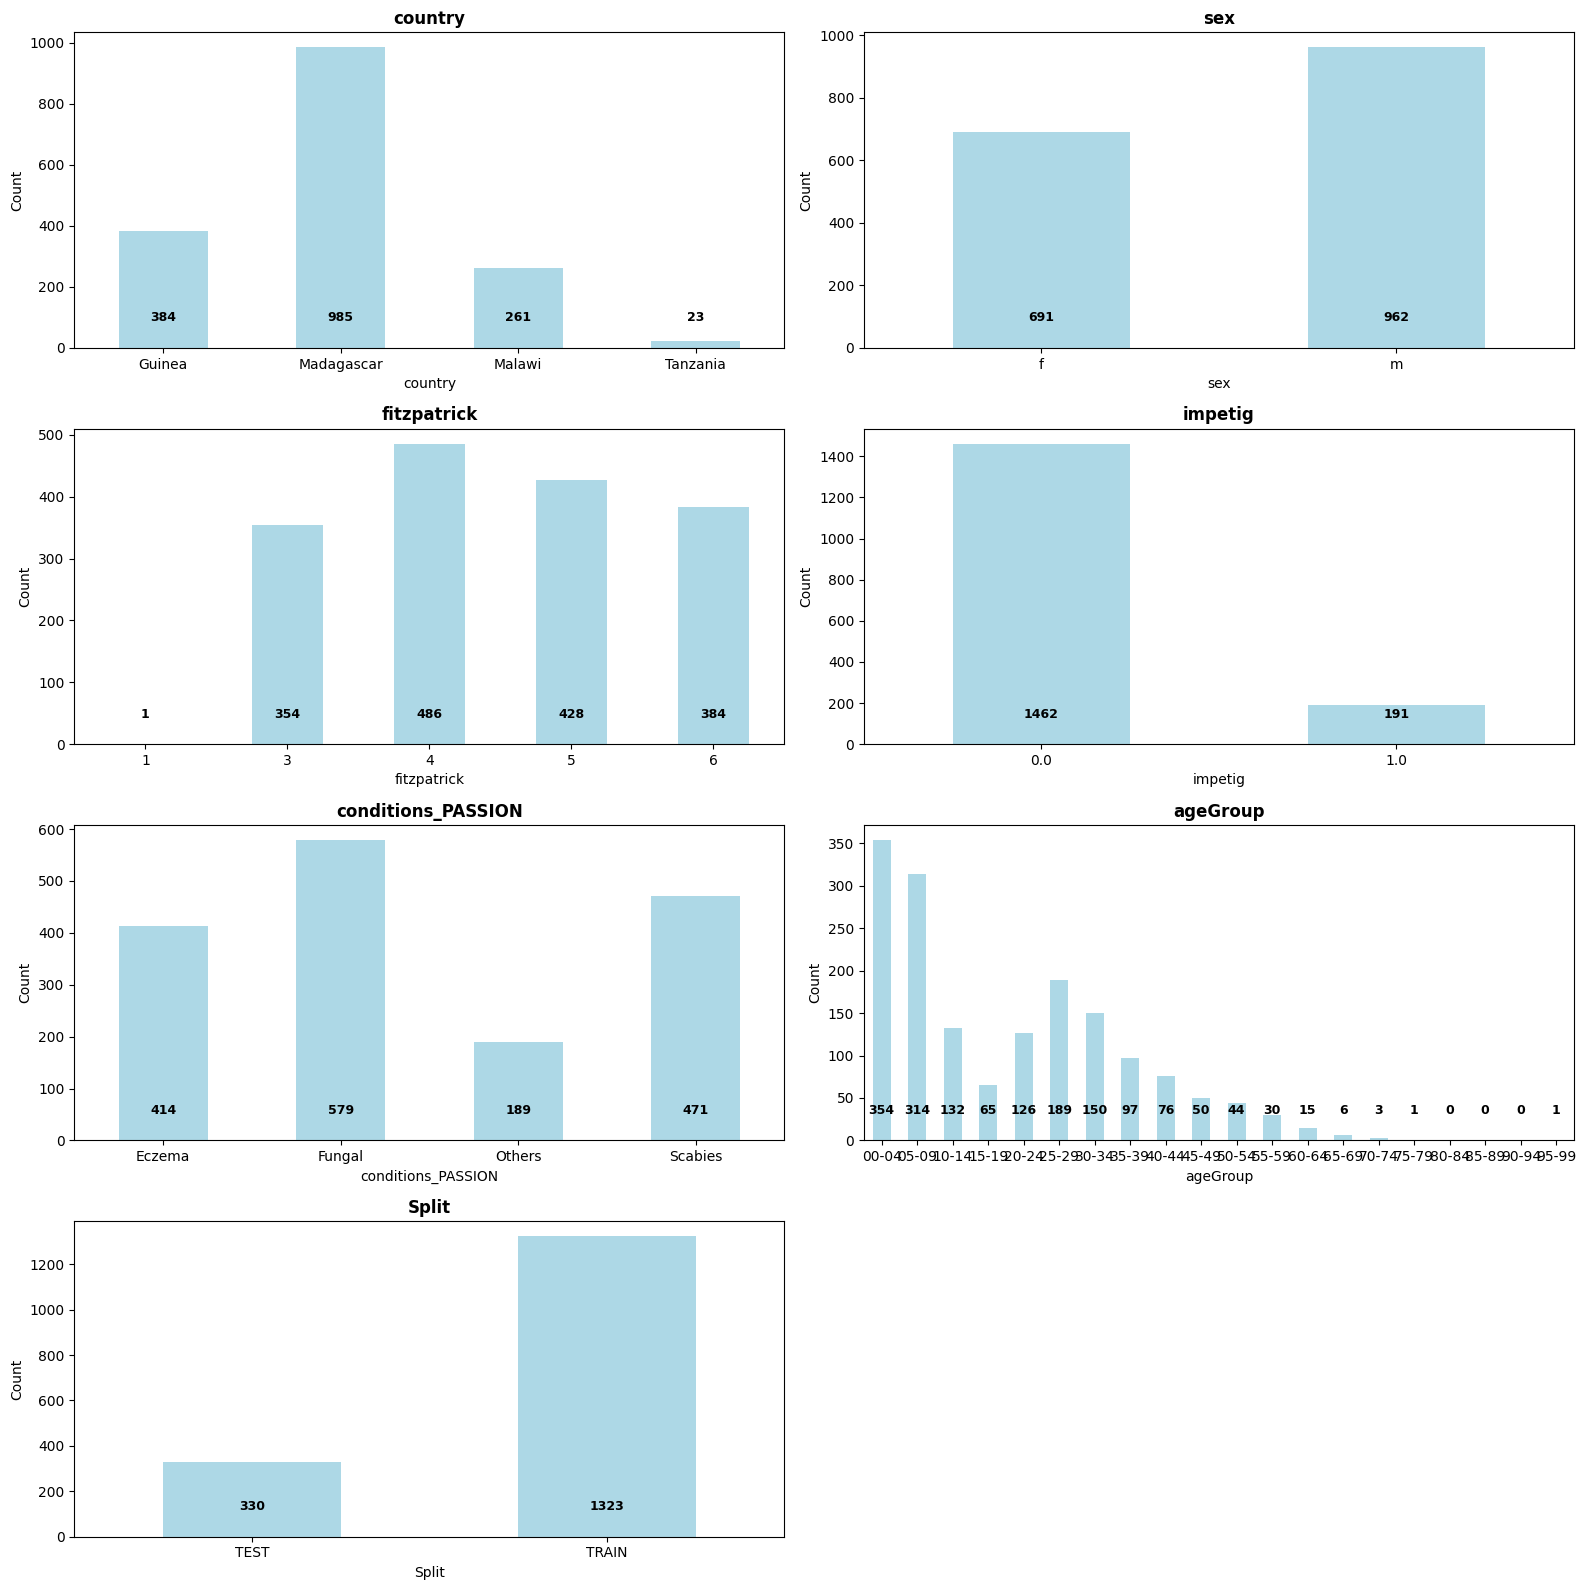
\includegraphics[width=0.9\textwidth]{figures/PASSION_split_all_distributions.png}
				\caption{PASSION dataset distribution analysis on group level}
				\label{fig:PASSIONDatasetDistrAnalysis}
			\end{figure}
			
			\begin{table}[H]
				\centering
				{
					\catcode`\_=12
					\csvautobooktabular{csvs/distribution_PASSION_split.csv}
					\catcode`\_=8
				}
				\caption{Distribution of metadata attributes in the PASSION dataset}
				\label{tbl:PASSIONDatasetDistrAnalysis}
			\end{table}
		\end{appendices}
		
		
		
			
		\glsaddallunused                                % add all unused items to glossary
		\todo{check the gls all unused.}
		
	
\end{document}
